\documentclass[review]{elsarticle}
\usepackage[table,dvipsnames,svgnames,x11names]{xcolor}
\usepackage{color}
\definecolor{c1}{rgb}{241,238,246}
\definecolor{c2}{rgb}{208,209,230}
\definecolor{c3}{rgb}{166,189,219}
\definecolor{c4}{rgb}{116,169,207}
\definecolor{c5}{rgb}{43,140,190}
\definecolor{c6}{rgb}{4,90,141}
\usepackage{amsthm}
\newtheorem{myDef}{Definition}
\newtheorem*{OtherDef}{Definition}
\newtheorem{myTheo}{Theorem}
\newtheorem{myPrp}{Property}
\newtheorem{myLem}{Lemma}
\newtheorem*{myPrf}{Proof}
\newtheorem{myPre}{Preposition}
%\usepackage[toc,page]{appendix}
\usepackage[section]{algorithm}
\usepackage{algpseudocode}
\usepackage[fleqn]{amsmath}
\usepackage{amssymb}
\usepackage{graphics}
\usepackage{epsfig}
\usepackage{setspace}
\usepackage{lineno,hyperref}
\usepackage{bm}
\usepackage{cleveref}
\usepackage{caption}
%\usepackage{cite}
\usepackage{graphicx} %???????
\usepackage{float} %???????????
\usepackage{subfigure} %?????????????
\usepackage{multirow}
\usepackage{rotfloat}

\modulolinenumbers[5]
\renewcommand{\algorithmicrequire}{\textbf{Input:}} %Use Input in the format of Algorithm
\renewcommand{\algorithmicensure}{\textbf{Output:}} %UseOutput in the format of Algorithm
\journal{Information Sciences}
%%%%%%%%%%%%%%%%%%%%%%%
%% Elsevier bibliography styles
%%%%%%%%%%%%%%%%%%%%%%%
%% To change the style, put a % in front of the second line of the current style and
%% remove the % from the second line of the style you would like to use.
%%%%%%%%%%%%%%%%%%%%%%%
%% Numbered
%\bibliographystyle{model1-num-names}
%% Numbered without titles
%\bibliographystyle{model1a-num-names}
%% Harvard
%\bibliographystyle{model2-names.bst}\biboptions{authoryear}
%% Vancouver numbered
%\usepackage{numcompress}\bibliographystyle{model3-num-names}
%% Vancouver name/year
%\usepackage{numcompress}\bibliographystyle{model4-names}\biboptions{authoryear}
%% APA style
%\bibliographystyle{model5-names}\biboptions{authoryear}
%% AMA style
%\usepackage{numcompress}\bibliographystyle{model6-num-names}
%% `Elsevier LaTeX' style
\bibliographystyle{elsarticle-num}
%%%%%%%%%%%%%%%%%%%%%%%
\begin{document}
\captionsetup[figure]{labelfont={bf},labelformat={default},labelsep=period,name={Fig}}	
\captionsetup[table]{labelfont={bf},labelformat={default},labelsep=period,name={Table}}
\begin{frontmatter}
\title{Improved General Attribute Reduction Algorithms for Inconsistent Decision Table}
%% or include affiliations in footnotes:
\author[mymainaddress]{Baizhen Li}
\author[mymainaddress]{Zhihua Wei\corref{mycorrespondingauthor}}
\author[mymainaddress]{Duoqian Miao}
\author[mysecondaryaddress]{Nan Zhang}
\author[mymainaddress]{Wen Shen}
\author[mymainaddress]{Hongyun Zhang}
\author[mymainaddress]{Lijun Sun}
\cortext[mycorrespondingauthor]{corresponding author: zhihua\_wei@tongji.edu.cn}
\address[mymainaddress]{Tongji University, Shanghai 201804, PR China}
\address[mysecondaryaddress]{Yantai University, Yantai, Shandong 264005, PR China}

\begin{abstract}
Attribute reduction is a key issue in rough set theory. In recent years, many kinds of attribute reduction have been proposed, such as positive region preservation reduction, generalized decision preservation reduction, distribution preservation reduction, maximum distribution preservation reduction, and relative discernibility relation preservation reduction. General reduction approaches to obtain various types of reducts also have been explored, but it is computationally time-consuming in the condition of large-scale data. In this study, we focus on the efficient general reduction algorithm to obtain five typical reducts mentioned above. At first, we introduce a concept named granularity space to establish a unified representation of five typical reducts. Based on the unified representation, we construct two quick general reduction algorithms by extending the positive region approximation to the granularity space. We conduct a series of comparisons in aspects of theoretical analysis and experiments to evaluate the performance of two algorithms. The results of the theoretical analysis and experiments indicate that two general reduction algorithms proposed in this study are effective and efficient.
\end{abstract}

\begin{keyword}
Attribute reduction, Granularity computing, Inconsistent decision table, Rough set
\MSC[2019] 00-01\sep  99-00
\end{keyword}
\end{frontmatter}

\linenumbers

\section{Introduction}
	\par Rough set theory, introduced by Z. Pawlak \cite{Pawlak1982} in 1982, is an efficient tool to imprecise, incomplete and uncertain information processing \cite{Huang2016,Dai2012,Shi2016,zhan2017}. Currently, rough set theory has been successfully applied to many practical problems, including machine learning \cite{das2016ierspop,xie2018test}, pattern recognition \cite{hu2015flow,huang2012enhanced}, data mining \cite{wang2013attribute}, decision support systems \cite{kaya2013hybrid}, etc.
	
	\par Attribute reduction, the process of obtaining a minimal set of attributes that can preserve the same ability of classification as the entire attribute set, is one of the core concepts in rough set theory \cite{thangavel2009}. Main studies of attribute reduction can be classified into two categories: the appropriate definition of attribute reduction and the efficient reduction algorithm.
	
	\par The appropriate definition of attribute reduction is a prerequisite for the good performance of attribute reduct in classification. After analyzing the relation of the positive region and classification rule in the consistent decision table, Pawlak proposed the positive region preservation reduction \cite{Pawlak1982}. Kryszkiewicz proposed two reductions for inconsistent decision tables: the generalized decision preservation reduction and the distribution preservation reduction \cite{kryszkiewicz2001comparative}, which guarantee the property of possible decisions of objects and the decision class membership distribution of objects unchanged. After that, Zhang et al. \cite{zhang2003knowledge} presented the maximum distribution preservation reduction as a compromise between the capability of generalized decision preservation reduction and the complexity of distribution preservation reduction. Since then, designing appropriate attribute reduction definitions based on understanding the relationship between the different attribute reductions became one of research focus. Liu et al. \cite{liu2006knowledge} presented the distribution preservation reduction, the maximum distribution preservation reduction, and the generalized decision preservation reduction in the way of the classic reduction. Furthermore, Ref \cite{miao2009relative} classified existing reductions into three types: the region preservation reduction, the decision preservation reduction, and the relationship preservation reduction. Then, Zhou et al. \cite{zhou2011analysis} reviewed the existing attribute reductions for the complete decision table and concluded that there are six different types of attribute reduction for inconsistent decision tables. On this basis, Jia et al. \cite{jia2016generalized} explored the general reduction definition. On the other side, Li et al. \cite{li2014quick} paid attention to the computational efficiency of reduction definition and designed new definitions to speed up attribute reduction. On reviewing the discernibility relation, Ge et al. \cite{ge2017quick} proposed a common definition of five types of attribute reduction for inconsistent decision tables.
	
	\par The efficient reduction algorithm \cite{li2009approaches,meng2009fast,guoyin2001rough,wei2010relation} is the central focus of researchers. Attribute reduction methods can be grouped into two classes \cite{thangavel2009dimensionality}: the discernibility matrix-based method \cite{skowron1991towards,skowron1992discernibility} and the heuristic method. Many researchers studied attribute reduction algorithms using the discernibility matrix because it is easily understanding and can find all reducts \cite{kryszkiewicz2001comparative,zhang2003knowledge,miao2009relative,zhou2011analysis,deng2006new,wang2001reduction,xu2009efficient,yao2009discernibility}. However, the discernibility matrix-based method is computationally expensive. Therefore, heuristic approaches are applied to attribute reduction processes. The heuristic approach is composed of two parts: the attribute reduction heuristic and the search strategy \cite{yao2008reduct}. The attribute reduction heuristic is the fitness function of a heuristic approach. Existing definitions of heuristics are mainly based on three aspects: dependency degree \cite{hu1995learning}, entropy \cite{tian2013rough,Sun2017Continuous,Yan2017Entropy}, and consistency \cite{Dash2003Consistency,Hu2007Consistency}. The search strategy is the control structure of the heuristic approach. There are two basic search strategies in heuristic approaches \cite{Wang1998Analysis}: the directional search strategy and the non-directional search strategy. The directional search strategy contains three kinds of methods: the deletion method, the addition method, and the addition-deletion method. The non-directional search strategy is usually applied in evolutionary algorithms \cite{jia2013minimum,liu2010adaptive,shi2006heuristic,deng2009improved,ke2008efficient,dai2006particle} and some optimization methods \cite{hedar2008tabu,yu2011solving,jensen2004semantics,ye2007new}. To further increase computational efficiency, many researchers studied acceleration mechanisms of the heuristic attribute reduction method. Ref \cite{ge2017quick,liu2003research,xu2006quick} computed equivalence classes using a classic sort algorithm, which improved the performance of attribute reduction algorithms. Qian et al. \cite{qian2011hybrid} presented a counting sort algorithm to reduce the computation cost of positive regions and core attributes. Furthermore, Qian et al. \cite{qian2010positive} studied an acceleration strategy for the positive region preservation reduction and three types of entropy reductions in complete decision tables. Liang et al. \cite{liang2013accelerator} developed a new accelerator that simultaneously decreased the size of the universe and the number of attributes in each iteration process of attribute reduction.
	
	\par There are five representative reductions for complete inconsistent decision tables, \emph{i.e.} positive region preservation reduction, generalized decision preservation reduction, distribution preservation reduction, maximum distribution preservation reduction, and relative discernibility relation preservation reduction. General attribute reduction approaches to obtain five types of reducts have been explored in \cite{ge2017quick}. However, existing general reduction algorithms are still computationally time-consuming in processing large-scale data. To alleviate this problem, we propose two quick general reduction algorithms to obtaining five types of reducts for inconsistent decision tables. 
	Firstly, To construct the general attribute reduction definition, we introduce the concept of granularity space and analyze the properties of its binary relation. Subsequently, by associating the indiscernibility relation of granularity space with the indiscernibility relation of five reducts, we construct the general attribute reduction definition in the way of granularity space. Finally, based on extending the positive region approximation to the granularity space, we develop two quick general reduction algorithms. Meanwhile, a series of analyses in aspects of theory and experiments are conducted to evaluate the effectiveness and efficiency of proposed algorithms. 
	Two major contributions of this study are: (1) We introduce a concept named granularity space which can represent five attribute reductions in a unified framework; (2) We extend the positive region approximation to the granularity space and design a new acceleration strategy for general attribute reduction algorithms, which can expand the acceleration domain from the positive region to the universe of the decision table.
	
	\par The rest of this paper is organized as follows. In section 2, we briefly review preliminary notions related to reduction and five representative reductions for the inconsistent decision tables. In section 3, we give the corresponding notions of the granularity space and presents the quick general heuristic reduction algorithm based on granularity space. In section 4, we construct a series of experiments with several UCI data sets to evaluate the performance of proposed reduction algorithms. Finally, section 5 concludes this paper and brings some remarks about the work of this paper.
	
\section{Preliminaries}
	\par This section would briefly review some preliminary notions about five representative attribute reductions for inconsistent decision tables, and present some details about the discernibility matrix-based reduction method.
	\par The research object of the rough set theory is called the information system. The information system $IS$ can be expressed as $IS=<U,A,V,f>$, where $U$ stands for the universe of discourse, a non-empty finite set of objects. $A$ is the set of attributes, $V=\bigcup_{a \in A}V_{a}$ is the set of all attribute values, and $f:U \times A \rightarrow V$ is the information function. For $\forall x \in U$ and $\forall a \in A$, we have $f(x,a) \in V_a$. The information system that satisfies $A=C \cup D$ and $C \cap D = \emptyset$ is also called the decision table, where $C$ is a set of conditional attributes, and $D$ is a set of decision attributes.
	\par For conditional attribute set $B \subseteq C$ in the decision table, the indiscernibility relation $IND(B)$ is defined by $IND(B) = \{<x,y> \in U \times U|f(x,a)=f(y,a), \forall a \in B\}$. For every $x \in U$, the equivalence class of $x$, denoted by $[x]_B$, is defined by $[x]_B = \{ y \in U|<x,y> \in IND(B)\}$. The family of all equivalence classes of $IND(B)$, \emph{i.e.}, the partition determined by $B$, is denoted by $U/IND(B)$ or simply $U/B$. $X$, a non-empty subset of $U$, is called a concept of $U$. The $B$-lower approximation $\underline{B}(X)$ and $B$-upper approximation $\overline{B}(X)$ of $X$ are defined by $\underline{B}(X) = \{x \in U|[x]_B \subseteq X\}, \overline{B}(X) = \{x \in U|[x]_B \cap X \neq \emptyset\}$.
	\par The classification ability of conditional attribute $C$ is measured by the relation of $IND(C)$ and $IND(D)$, and there are some uncertain situations that objects $x,y$ with the same conditional attributes value perform differently in the decision attributes value. In rough set theory, it is represented as the difference of two concepts induced from indiscernibility relation and addressed by concept approximation which called positive region and boundary region. Let all elements of $U/D$ be the target concepts we want to represent, the $B$-positive region $POS_B(D)$ and $B$-boundary region $BND_B(D)$ in the relation $IND(B)$ can be defined as follows.
		\begin{equation*}\begin{split}
			&POS_B(D) = \bigcup_{X \in U/D}\underline{B}(X).\\
			&BND_B(D)=\bigcup_{X \in U/D} (\overline{B}(X)-\underline{B}(X)).
		\end{split}\end{equation*}
	$POS_B(D), BND_B(D)$ presents objects containing certainty information and uncertainty information. There are some extensions of the positive region for characterizing the classification ability from different perspectives. For the convenience of comparison, we list five typical reduction definitions summarized in Ref \cite{zhou2011analysis} as follows.
	\par Given a decision table $DT=(U,C,D,V,f)$, $B \subseteq C$ is called\\
	\rm{(1)} $B$ is a positive region preservation reduct (denoted as PRPR) of $C$ with respect to $D$ iff $B$ satisfies $\ POS_B(D)=POS_C(D)$ and $\ \forall B' \subset B,\ POS_{B'}(D) \neq POS_{C}(D)$.\\
	\rm{(2)} $B$ is a generalized decision preservation reduct (denoted as GDPR) of $C$ with respect to $D$ iff $B$ satisfies $\forall x\in U, \delta_{B}(x)=\delta_{C}(x)$ and $\forall B' \subset B, \exists x \in U, \delta_{B'}(x) \neq \delta_{B}(x)$, where $\delta_{B}(x)=\{f(y,d)| x \in U \wedge y \in [x]_B\}$.\\
	\rm{(3)} $B$ is a distribution preservation reduct (denoted as DPR) of $C$ with respect to $D$ iff $B$ satisfies $ \forall x\in U, \mu_{B}(x)=\mu_{C}(x)$ and $\forall B' \subset B, \exists x \in U, \mu_{B'}(x) \neq \mu_{B}(x)$, where $\mu_{B}(x)=(P(D_1|[x]_B),P(D_2|[x]_B),\cdots,P(D_{|U/D|}|[x]_B)),P(D_j|[x]_B)=\frac{|D_j \cap [x]_B|}{|[x]_B|}, x \in U, D_j \in U/D(j=1,2,\cdots,|U/D|)$.\\
	\rm{(4)} $B$ is a maximal distribution preservation reduct (denoted as MDPR) of $C$ with respect to $D$ iff $B$ satisfies $\forall x \in U, \phi_{B}(x)=\phi_{C}(x)$ and $\forall B' \subset B, \exists x \in U, \phi_{B'}(x) \neq \phi_{B}(x)$, where $\phi_{B}(x)=\{D_{j}|\frac{|[x]_B \cap D_{j}|}{|[x]_{B}|}=\max\limits_{k=1}^{|U/D|}\{\frac{|[x]_B \cap D_{k}|}{|[x]_{B}|}\}\}$.\\
	\rm{(5)} $B$ a relative discernibility relation preservation reduct (denoted as DRPR) of $C$ with respect to $D$ iff $B$ satisfies
	$IND(B|D)=IND(C|D)$ and $\forall B' \subset B, IND(B'|D) \neq IND(B|D)$, where $IND(B|D)=\{(x,y)\in U \times U| (\forall a \in B \rightarrow f(x,a)=f(y,a)) \vee f(x,d)=f(y,d)\}$. 
	\par Attribute reduction algorithms, the process of obtaining reduct $B$, can be classified into two groups: the discernibility matrix-based algorithm and the heuristic algorithm. For the limitation of paper focus, here we just review the discernibility matrix-based algorithm. A general discernibility matrix given by Miao et al. \cite{miao2009relative} is defined as follows:
	\par Given a decision table $DT=(U,C,D,V,f)$, its discernibility matrix $DM=(DM(x,y))$ is a $|U| \times |U|$ matrix. $DM(x,y)$ for an object pair $(x,y)$ is $\{a \in C|<x,y> \in DIS(C|D), f(x,a)\neq f(y,a)\}$, where $DIS(C|D)$ is the relative discernibility relation. The relative discernibility relation of five typical reducts for inconsistent decision tables can be written as follows.
	\\\rm{(1)} The relative discernibility relation of PRPR is defined by $DIS(C|D)=\{<x,y>|x,y \in POS_C(D) \wedge f(x,D)\neq f(y,D) \vee x \in POS_C(D) \wedge y \not \in POS_C(D) \}$;
	\\\rm{(2)} The relative discernibility relation of GDPR is defined by $DIS(C|D)=\{<x,y>| \delta_{C}(x) \neq \delta_{C}(y)\}$;
	\\\rm{(3)} The relative discernibility relation of DPR is defined by $DIS(C|D)=\{<x,y>|\mu_{C}(x)\neq \mu_{C}(y)\}$;
	\\\rm{(4)} The relative discernibility relation of MDPR is defined by $DIS(C|D)=\{<x,y>| \mu_{C}(x)\neq \mu_{C}(y)\}$;
	\\\rm{(5)} The relative discernibility relation of DRPR is defined by $DIS(C|D)=\{<x,y>| f(x,C)\neq f(y,C) \wedge f(x,D) \neq f(y,D)\}$.
	\par Based on the discernibility matrix, one can get the reduct through the following discernibility function. $f(DM)=\bigwedge \{\bigvee(DM(x,y))| \forall x,y \in U, DM(x,y) \neq \emptyset\}$. The expression $\bigwedge \{\bigvee(DM(x,y)))\}$ is the conjunction of all $\bigvee(DM(x,y))$ while $\bigvee(DM(x,y))$ is the dis-junction of condition attributes in $DM(x,y)$. The discernibility function can be transformed to a reduced disjunctive, and each conjunctor of the reduced disjunctive form is a reduct or super set of reduct.

\section{Granularity space and the quick general reduction algorithm}
	In this section, We represent the definition of five typical reducts in a unified way and develop two quick general reduction algorithms. 
	In subsection \ref{granularitySpace}, we introduce a new concept named granularity space and analyze the discernibility relation and indiscernibility relation of granularity space. By associating the indiscernibility relation of granularity space with the indiscernibility relation of five reducts, we construct the common representation of five reducts using granularity space.
	In subsection \ref{subsection.gs}, we extend the positive region approximation to granularity space and design a new acceleration strategy named granularity approximation, which expands the acceleration domain from the positive region to the universe of the decision table. Based on granularity approximation, we develop two quick general reduction algorithms.
	In subsection \ref{ag}, we make the comparison of the existing general reduct definition and the general reduct defined by granularity space in aspects of simplicity and intuition. For easily understanding of proposed algorithms, we provide a calculation example for obtaining positive region preservation reduct in the end of subsection.
	\subsection{Granularity space: an alternative of general attribute reduct definition}\label{granularitySpace}
		Given a non-empty finite set $U$, a partition or granularity $G$ of $U$ is defined as follows:
		\begin{equation*}G= \{C_i|\bigcup_{C_i \subset G} C_i=U \wedge(C_i \cap C_j=\emptyset,i \neq j)  \}\end{equation*}
	For the convenience of writing, we term $G$ as a granularity of $U$, or simply a granularity.
		\begin{myDef}
			Given a granularity $G$ of a finite non-empty set $U$, the indiscernibility relation and the discernibility relation of $G$ is defined as follows.
			\begin{equation*}IND(G)=\{<x,y>|<x,y>\in C_i \times C_i \wedge C_i \in G\}\end{equation*}
			\begin{equation*}DIS(G)=\{<x,y>|(<x,y>\in C_i \times C_j,i \neq j)\wedge C_i,C_j \in G\}\end{equation*}
		\end{myDef}
		The indiscernibility relation of the granularity $G$ of $U$ satisfies:
			\\{\rm(1)} Symmetric: $\forall x \in U,\;<x,x>\in IND(G)$.
			\\{\rm(2)} Transitive: $\forall x,y,z \in U$, if $<x,y>,<y,z> \in IND(G)$, then $<x,z> \in IND(G)$.
			\\{\rm(3)} Reflexive: $\forall x,y \in U$,if $<x,y> \in IND(G)$, then $<y,x> \in IND(G)$.\\
		The discernibility relation of a granularity $G$ of $U$ satisfies reflexive, \emph{i.e.} for $\forall x,y \in U$, if $<x,y> \in DIS(G)$, then $<y,x> \in DIS(G)$.
		Things needed to be reminded of are $IND(G) \cup DIS(G) = \{<x,y>|<x,y>\in U \times U\}$ and $\{G|G=U/B,B\subseteq C\}\subseteq \{G|G \; is \; a \; granularity \; of \; U\}$.
		\begin{myDef}\label{gspace}
			Granularity space can be represented in 2-tuples $GS=(G,O)$, where $G$ is a granularity of a finite non-empty set $U$, $O$ is a set of operators on element of $G$. the ancenstor granularity space of $G$ is defined by $ANC(G)=(G,\{\cup\})$; the granularity subspace of $G$ is defined by $SPR(G)=(G,\{\propto\})$, where $\propto U=\{P,Q|P\cup Q=U \wedge P \cap Q= \emptyset\}$.
		\end{myDef}
		Granularity space is the set of granularity generated from doing several operations specified by $O$ on $G$. Specially, let $G \in (G,\{\propto\}), G \in (G,\{\cup\})$. As a result, we can construct following lemma.
		\begin{myLem}\label{bAK}
			Given a partition granularity $G$ of a finite non-empty set $U$, for $\forall G' \in ANC(G)$, we have $IND(G') \supseteq IND(G),DIS(G') \subseteq DIS(G)$; for $\forall G' \in SPR(G)$, we have $IND(G') \subseteq IND(G),DIS(G') \supseteq DIS(G)$.
		\end{myLem}
		\begin{myPrf}
			We know that $IND(G) \cup DIS(G) = U \times U,\;IND(G) \cap DIS(G)=\emptyset$, so all we need to do for proving Lemma \ref{bAK} true are proving true either $\forall G' \in ANC(G), IND(G') \supseteq IND(G)$ or $\forall G' \in SPR(G)$, $IND(G') \subseteq IND(G)$. Given $G' \in ANC(G)$, according to Definition \ref{gspace}, we know that $\forall E \in G'$, there exists a set $PE$ such that $\bigcup_{P_i \in PE}P_i=E$. So $\emptyset \subseteq \{<x,y>| x \in P_i \in PE, y \in \bigcup_{P_j \in PE-P_i}P_j,\;P_i,P_j \in PE,x,y\in E\} \Rightarrow DIS(G') \subseteq DIS(G)$. That is to say, Lemma \ref{bAK} is true.
		\end{myPrf}
		\noindent\textbf{Example 1}. Given $U=\{x_1,x_2,x_3\},G=\{\{x_1\},\{x_2,x_3\}\}$, then we know $ANC(G)=(G,\{\cup\})=\{G,U\}$. let $Q$ denotes $\{\{x_1\},\{x_2\},\{x_3\}\}$, $SPR(G)=(G,\{\propto\})=\{G,Q\}$.
		$IND(U)=U \times U, DIS(U)=\emptyset;\\ IND(G)=\{<x_1,x_1>,<x_2,x_2>,<x_3,x_3>,<x_2,x_3>,<x_3,x_2>\}, DIS(G)=\{<x_1,x_2>,<x_2,x_1>,<x_1,x_3>,<x_3,x_1>\},IND(Q)=\{<x_1,x_1>,<x_2,x_2>,<x_3,x_3>\},
		DIS(Q)=\{<x_1,x_2>,<x_2,x_1>,<x_1,x_3>,<x_3,x_1>,<x_2,x_3>,<x_3,x_2>\}$.
		\\It is obvious that $\forall G' \in ANC(G), IND(G) \subseteq IND(G')$ \emph{i.e.} $DIS(G) \supseteq DIS(G')$ and $\forall G' \in SPR(G), DIS(G) \subseteq DIS(G')$ \emph{i.e.} $DIS(G) \supseteq DIS(G')$.
		\begin{myTheo}\label{ancestorSpace}
			Given a decision table $DT=(U,C,D,V,f)$ and let $G=U/C$. For any type of reduct $B$, $U/B \in ANC(G)$.
		\end{myTheo}
		$U/B \in ANC(G)$ can be induced from $B \subseteq C$. For $\forall B \subseteq C$, if $y\in [x]_C$ then $y \in [x]_B$. Here we re-construct discernibility and indiscernibility relation of reducts from granularity perspective.
		\begin{myDef}
			Given a decision table $DT=(U,C,D,V,f)$ and reducts $\{PRPR,\\ GDPR, DPR, MDPR, DRPR\}$, the relative discernibility relation and the relative indiscernibility relation of the reduct are defined as follows:
			\begin{spacing}{0.6}
				\begin{equation}\begin{split}
					DIS(PRPR)=&\{<x,y>| y \not \in [x]_C \wedge (x,y \in POS_C(D) \wedge f(x,D) \neq \\&f(y,D) \vee  x \not \in POS_C(D) \wedge y \in POS_C(D))\}
				\end{split}\end{equation}
				\begin{equation}\begin{split}
					IND(PRPR)=\{&<x,y>|y \in [x]_C \vee y \not \in [x]_C \wedge (x,y \not \in POS_C(D)  \\
					& \vee x,y \in POS_C(D) \wedge f(x,D)=f(y,D) )  \}
				\end{split}\end{equation}
				\begin{equation}DIS(GDPR)=\{ <x,y>|y \not \in [x]_C \wedge \delta_C(x) \neq \delta_C(y) \} \end{equation}
				\begin{equation}IND(GDPR)\{<x,y>|y \in [x]_C \vee y \not \in [x]_C \wedge \delta_C(x) = \delta_C(y)\}\end{equation}
				\begin{equation}DIS(DPR)=\{<x,y>|y \not \in [x]_C \wedge \mu_C(x) \neq \mu_C(y)\}\end{equation}
				\begin{equation}IND(DPR)=\{<x,y>|y \in [x]_C \vee y \not \in [x]_C \wedge \mu_C(x) = \mu_C(y)\}\end{equation}
				\begin{equation}DIS(MDPR)=\{<x,y>|y \not \in [x]_C \wedge \phi_C(x) \neq \phi_C(y)\}\end{equation}
				\begin{equation}IND(MDPR)=\{<x,y>|y \in [x]_C \vee y \not \in [x]_C \wedge \phi_C(x) = \phi_C(y)\}\end{equation}
				\begin{equation}\begin{split}
					DIS(DRPR)=&\{<x,y>|y \not \in [x]_C \wedge(x \in BND_C(D) \vee y \in BND_C(D) \\
					&\vee x,y \in POS_C(D) \wedge f(x,D) \neq f(y,D)) \}
				\end{split}\end{equation}
				\begin{equation}
				IND(DRPR)=\{<x,y>|y \in [x]_C \vee x,y \in POS_C(D) \wedge f(x,D)=f(y,D)\}
				\end{equation}
			\end{spacing}
		\end{myDef}
		For the relative discernibility relation and relative indiscernibility relation of reduct, it is worth noting that $\forall Red \in \{PRPR, GDPR, DPR, MDPR, DRPR\}$, $IND(Red)$ satisfies following properties.
		\\{\rm(1)} Symmetric: $\forall x \in U, <x,x>\in IND(Red)$.
		\\{\rm(2)} Transitive: $\forall x,y,z \in U$, if $<x,y>,<y,z> \in IND(Red)$, then $<x,z> \in IND(Red)$.
		\\{\rm(3)} Reflexive: $\forall x,y \in U$, if $<x,y> \in IND(Red)$, then $<y,x> \in IND(Red)$.
		The discernibility relation $DIS(Red)$ is reflexive. That is to say, for $\forall x,y \in U$, if $<x,y> \in DIS(Red)$, then $<y,x> \in DIS(Red)$.
		By the way, it is easy to find that $DIS(Red) \cap IND(Red)=\emptyset$, $IND(Red) \cup DIS(Red) = U \times U$.
		\begin{myTheo}\label{redB}
			Given a decision table $DT=(U,C,D,V,f)$ and $B \subseteq C$, then we have\\
			{\rm(1)} $DIS(PRPR) \subseteq DIS(B) \Leftrightarrow POS_B(D)=POS_C(D)$;\\
			{\rm(2)} $DIS(GDPR) \subseteq DIS(B) \Leftrightarrow \forall x \in U, \delta_B(x)=\delta_C(x)$\\
			{\rm(3)} $DIS(DPR) \subseteq DIS(B) \Leftrightarrow \forall x \in U, \mu_B(x)=\mu_C(x)$\\
			{\rm(4)} $DIS(MDPR) \subseteq DIS(B) \Leftrightarrow \forall x \in U, \phi_B(x)=\phi_C(x)$\\
			{\rm(5)} $DIS(DRPR) \subseteq DIS(B) \Leftrightarrow IND(B|D)=IND(C|D)$\\
		\end{myTheo}
		\begin{myPrf}
			According to definitions of related reducts and discernibility matrix-based reduction method, it is easily to know that item {\rm(2)}, {\rm(3)}, {\rm(4)} of Theorem \ref{redB} are true. So here we just prove the correctness of item {\rm(1)}, {\rm(5)}. \\
			\rm(1) \textbf{Sufficiency}: Assume that $DIS(PRPR) \subseteq DIS(B)$ and $\exists x \in POS_C(D), x \not \in POS_B(D)$. It can be implied that $\exists y \in [x]_B, y \not \in [x]_C$ and $f(y,D) \neq f(x,D)$, so we have $<x,y> \in DIS(PRPR) \subseteq DIS(B)$ and $y \not \in [x]_B$. As a result, $DIS(PRPR) \subseteq DIS(B) \Rightarrow POS_B(D)=POS_C(D)$.\\
			\textbf{Necessity}: Assume that $POS_B(D)=POS_C(D)$ and $\exists <x,y> \in DIS(PR\\PR)$ such that $<x,y> \not \in DIS(B)$. If $x \in POS_C(D) \wedge y \in POS_C(D) \wedge f(x,D)\neq f(y,D)$, then we know $x \not \in POS_C(D)$. That is contradicted with $POS_B(C)=POS_C(D)$. If $x \in POS_C(D) \wedge y \not \in POS_C(D)$, then according to assumption we know $x \in [y]_B$, and that implies $POS_C(D) \neq POS_B(D)$. In summary, if  $POS_B(D)=POS_C(D)$, then we have $DIS(PRPR) \subseteq DIS(B)$. \\
			{\rm(5)} \textbf{Sufficiency}: Assume that $DIS(DRPR) \subseteq DIS(B)$ and $\exists <x,y> \not \in IND(C|D) \wedge <x,y> \in IND(B|D)$. That means $\exists y \not \in [x]_C, y\in [x]_B,f(x,D) \neq f(y,D)$. Then we know $<x,y> \in DIS(DRPR) \subseteq DIS(B)$, and it implies $y \not \in [x]_B$, which is contradicted with our assumption. Finally, we get $DIS(DRPR) \subseteq DIS(B) \Rightarrow IND(B|D) = IND(C|D)$.\\
			\textbf{Necessity}: Assume that $IND(B|D)=IND(C|D)$ and $\exists <x,y> \in DIS(RPR)$ such that $<x,y> \not \in DIS(B)$. If $y \not \in [x]_C \wedge(x \in BND_C(D) \vee y \in BND_C(D))$ then we have $\exists p\in[x]_C,\exists q\in[y]C, f(p,C) \neq f(q,C), f(p,D) \neq f(q,D)$. Because $<x,y> \in IND(B)$, we have $x\in [y]_B \Rightarrow p \in [q]_B$. We get $f(p,B)=f(q,B),<p,q> \not \in IND(B|D)$. It is contradicted with $IND(B|D)=IND(C|D)$. If $x,y \in POS_C(D) \wedge f(x,d) \neq f(y,d))$, then $<x,y> \in IND(B)$ means that $x \in [y]_B, <x,y>\not \in IND(B|D)$. It contradicts with $IND(C|D) \neq IND(B|D)$. In summary, $IND(B|D) = IND(C|D) \Rightarrow DIS(DRPR) \subseteq DIS(B)$.\\
		\end{myPrf}
		According to Theorem \ref{ancestorSpace}, \ref{redB} and Lemma \ref{bAK}, we can construct unified attribute definition using granularity space.
		\begin{myTheo}\label{generalReduct}
			Given a decision table $DT=(U,C,D,V,f)$ and reduct $Red \in \{PRPR, GDPR, DPR, MDPR, DRPR\}$. $B$ is a $Red$ of $C$, iff $B$ satisfies the following conditions:
			\\\indent{\rm(1)} $U/B \in ANC(U/C) \cap SPR(TGran(Red))$
			\\\indent{\rm(2)} $\forall B' \subset B$, $U/B'$ doesn't satisfy condition (1).\\
			where $TGran(Red)=U/IND(Red)$.
		\end{myTheo}
		 In fact, item $(1)$ can be written in short as $U/B \in SPR(TGran(Red))$ because of $\forall B \subseteq C, U/B \in ANC(U/C)$. Here we construct Algorithm \ref{computeTargetGranularity} for computing $TGran(Red), Red \in \{PRPR, GDPR, DPR, MDPR, DRPR\}$.
		\begin{algorithm}[htb]
			\setstretch{1}
			\caption{Calculating the target granularity algorithm(CTGA)}
			\label{computeTargetGranularity}
			\begin{algorithmic}[1]
				\Require decision table $DT=(U, C \cup D,V,f)$ and target reduct $Red \in \{PRPR,GDPR,DPR,MDPR,DRPR\}$
				\Ensure Target granularity of relative reduct.
				\State Compute $TG=U/C$
				\For{$ec1 \in TG$}
				\For{$ec2 \in TG-ec1$}
				\If{$<x,y>\in IND(Red): x \in ec1,y \in ec2$}
				\State $ec1:=ec1 \cup ec2$
				\State $TG=TG-ec2$
				\EndIf
				\EndFor
				\EndFor\\
				\Return $TG$
			\end{algorithmic}
		\end{algorithm}
		First part of $CTGA$ is getting the partition $U/C$ because $TGran(Red)$ is an element of $ANC(U/C)$. For the sake that $IND(Red)$ satisfies transitivity, algorithm \ref{computeTargetGranularity} scans all the combinations of $<e1,e2>, e1,e2 \in U/C$, and merges equivalence classes if $<x,y>\in IND(Red): x \in e1,y \in e2$. After the merging step, the result is $TGran(Red)$. For high efficiency of algorithm, we design a hash function for computing target granularity as follows.\\
		Given a decision table $(U,C,D,V,f)$, Let $U/D=\{D_1,D_2,\cdots,D_n\}$.\\
		{\rm(1)} $$ h(x,PRPR)=\left \{ \begin{aligned}&i ,\; if \; x \in POS_C(D) \wedge f(x,D)=D_i\\ &n+1 ,\; otherwise \end{aligned} \right. $$
		{\rm(2)} $h(x,GDPR)=\delta_C(x)$;\\
		{\rm(3)} $h(x,DPR)=\mu_C(x)$\\
		{\rm(4)} $h(x,MDPR)=\phi_C(x)$\\
		{\rm(5)} $$ h(x,DRPR)=\left \{ \begin{aligned}&i ,\; if \; x \in POS_C(D) \wedge f(x,D)=D_i\\ &f(x,C) ,\; otherwise \end{aligned} \right. $$\\
		Above hash function can be constructed in time complexity of $O(|U||C \cup D|)$ and we can efficiently compute target granularity resorting to a auxiliary hash function $H_a(h(x,Red))$, which map from $h(x,Red)$ to a set of objects. It is easily to know the upper bound of time complexity of computing $TGran(Red)$ using $CTGHF$ is $O(|U||C \cup D|+2|U|)$.
		\begin{algorithm}[htb]
			\setstretch{1}
			\caption{Calculating target granularity using hash function(CTGHF)}
			\label{CTGHF}
			\begin{algorithmic}[1]
				\Require decision table $DT=(U, C \cup D,V,f)$ and target reduct $Red \in \{PRPR,GDPR,DPR,MDPR,DRPR\}$
				\Ensure Target granularity of relative reduct in hash function way.
				\State Compute $U/C$
				\For{$ec \in U/C$}
				\State $t:=h(x,Red), H_a(t):= H_a(t) \cup \{x\}$, where $x \in ec$
				\EndFor\\
				\Return $H_a$
			\end{algorithmic}
		\end{algorithm}
		
	\subsection{Granularity search: an efficient general reduction method}\label{subsection.gs}
	\par Based on the general representation of five typical reducts presented in Theorem \ref{generalReduct}, we present a heuristic function called granularity approximation for efficient attribute reduction algorithms at first. Next, we propose two quick general attribute reduction algorithms for the inconsistent decision table.
	\begin{myDef}\label{granularityApproximation}
		Given a decision table $DT=(U,C,D,V,f)$ and a granularity $G$ of $U$. Let $[x]_G$ denotes a set of objects that belong to the same set in $G$. The granularity approximation of $G$ in $U/B$ is defined as follows.
		\begin{equation}
		GA(U/B,G) = \bigcup \{[x]_B|[x]_B \subseteq [x]_G\}
		\end{equation}
	\end{myDef}
	If you take $G$ as equivalence classes determined by attributes set $A$, granularity approximation can be written as $POS_B(A)$. It is consistent with the uncertainty processing measurement in Pawlak attribute reduction. Obviously, if $GA(U/B, TGran(Red))=U$ then $U/B \in SPR(TGran(Red))$. Thus, General reduct definition \ref{generalReduct} can be re-written as follows.
	\begin{myTheo}
		Given a decision table $DT=(U,C,D,V,f)$ and the target granularity $TGran(Red), \; Red \in \{PRPR, GDPR, DPR, MDPR, DRPR\}$. $B$ is a $Red$ of $C$, iff $B$ satisfies \\
		%\textbf{Granularity approxmation}: 
		\rm{(1)} $GA(U/B,TGran(Red))=U$\\
		\rm{(2)} $\forall B' \subset B$, $GA(U/B',TGran(Red)) \neq U$.%\\
		%\textbf{Conditional entropy}: $H(TGran(Red)|B)=0$ and $\forall B' \subset B$, $ H(TGran(Red)|B)>0$.
	\end{myTheo}
	For the granularity $G$ of $U$, it is easy to know that $\forall P \subseteq Q \subseteq C, GA(U/P,G) \subseteq GA(U/Q,G)$. According to Definition \ref{granularityApproximation}, the attribute significance for given attribute sets can be defined as follows.
	\begin{myDef}
		Given $DT=(U,C,D,V,f)$ and target granularity $G$. The weeded significance of $a \in B\subseteq C$ in $B$ for $G$ is defined as:
		\begin{equation}
		Sig^-(a,B,G)=|GA(U/B,G)-GA(U/B-\{a\},G)|
		\end{equation}
		the joined significance of $a \in C-B$ in B for $G$ is defined as:
		\begin{equation}
		Sig^+(a,B,G)=|GA(U/B\cup \{a\},G)-GA(U/B,G)|
		\end{equation}
		where $|A|$ denotes the cardinality of set $A$.
	\end{myDef}
	\par To increase the computation efficiency of the significance function, we explore the faster approach with the deletion of objects unrelated to the calculation. For the convenience of writing, we use $Sig^+(a,B,G,U)$ to represent the attribute significance, which denotes the value of the significance measure on the universe $U$. One can prove the following theorem of rank preservation.
	\begin{myTheo}
		Let $DT=(U,C,D,V,f)$ be a decision table, $B \subseteq C$ and $G$ is a granularity of $U$, $U'=U-GA(U/B,G)$. For $\forall a,b\in C-B$, if $Sig^+(a,B,G,U) \leq Sig^+(b,B,G,U)$, then $Sig^+(a,B,G,U')\leq Sig^+(b,B,G,U')$.
	\end{myTheo}
	\begin{myPrf}
		From the definition of $Sig^+(a,B,G,U)$, we know that its value only depends on the function $GA(U/B,G)$. Since $U'=U-GA(U/B,G)$, one can know $GA(U'/B,G)=GA(U/B\cup\{a\},G)-GA(U/B,G)$. Therefore, we have
		\begin{equation*}
		\frac{Sig^+(a,B,G,U)}{Sig^+(a,B,G,U')}=\frac{|GA(U/B\cup\{a\},G,U)-GA(U/B,G,U)|}{|GA(U/B\cup\{a\},G,U')-GA(U/B,G,U')|}=1
		\end{equation*}
		So $Sig^+(a,B,G,U)>Sig^+(b,B,G,U) \Leftrightarrow Sig^+(a,B,G,U')>Sig^+(b,B,G,U')$.
	\end{myPrf}
	Now we can construct the attribute reduction algorithm based on granularity approximation as follows. 
	\begin{algorithm}[htb]
		\setstretch{1}
		\caption{Granularity Search(GS)}
		\label{GS}
		\begin{algorithmic}[1]
			\Require decision table $DT=(U, C \cup D,V,f)$ and target reduct $Red \in \{PRPR, GDPR, DPR, MDPR, DRPR\}$
			\Ensure A reduct of $C$
			\State Compute the target granularity $G$ according to algorithm \ref{CTGHF};
			\State Compute $Sig^-(a_k,C,G,U),k \leq |C|$;
			\State Put $a_k$ into $core$, where $Sig^-(a_k,C,G,U)>0$;
			\State $red:=core,i:=0$ and $U_0:=U$;
			\While{$|U_i|>0$}
			\State Calculate $a_{max}:a_{max}=arg \max_{a \in C-red}Sig^+(a,red,G,U_{i+1})$;
			\State $red:=red \cup \{a_{max}\}$;
			\State Compute $U_{i+1}:=U_i-GA(U_i/red,G,U_i)$;
			\State $i:=i+1$;
			\EndWhile\\
			\Return $red$
		\end{algorithmic}
	\end{algorithm}
	\par Speaking loosely, the granularity search algorithm consists of four parts: computing target granularity, calculating core attributes, getting an attribute with maximal significance, and stopping judge. The complexity of computing $TGran(Red)$ is $O(|U||C\cup D|+2|U|)$; the complexity of calculating core attributes is $O(|U||C|^2)$; the complexity of remaining steps is $O(\sum_{i=1}^{|C-cr|}|U_i|(|cr|+i+1))$,where $cr$ denotes the set of core attributes.
	According to attribute reduction algorithm in Ref \cite{li2014quick}, the granularity search algorithm can be simplified to further increase the time efficiency by removing the part of computing core attributes and the attribute with maximal significance. For convenience, we denote granularity search without computing core attributes and the attribute with maximal significance as GSV. 
	\begin{algorithm}[htb]
		\setstretch{1}
		\caption{A Granularity Search Variant(GSV)}
		\label{GSV}
		\begin{algorithmic}[1]
			\Require decision table $DT=(U, C \cup D,V,f)$ and target reduct $Red \in \{PRPR, GDPR, DPR, MDPR, DRPR\}$
			\Ensure A reduct of $C$
			\State Compute the target granularity $G$ according to algorithm \ref{CTGHF};
			\State $red:=\emptyset, i:=0$ and $U_0:=U$;
			\While{$|U_i|>0$}
			\State $flag=False$;
			\For{$a \in C-red$}
			\If{$Sig^+(a,red,G,U_i) > 0$}
			\State $flag=True$;
			\State $red:=red \cup \{a\}$;
			\State Compute $U_{i+1}:=U_i-GA(U_i/red,G,U_i)$;
			\State $i:=i+1$;
			\EndIf
			\EndFor
			\If{$flag$ is False and $|U_i|>0$}
			\State $red:=red \cup \{a_0\}$;//$a_0$ is an arbitrary attribute of $C$
			\EndIf
			\EndWhile\\
			\Return $red$
		\end{algorithmic}
	\end{algorithm}
	
	\par We present the comparison of the upper bound of relevant algorithms time complexity in Table \ref{complexity}, in which "/" denotes that the step do not exist in this algorithm. QGARA-FS and QGARA-BS are general reduction algorithms proposed in Ref \cite{ge2017quick}. Taking into consideration the reduction results of QGARA-BS and GSV are partly detemined by the attribute order scanned, we divide four algorithms into two groups for comparison. One is GS $\emph{vs.}$ QGARA-FS; Another is GSV $\emph{vs.}$ QGARA-BS. The upper bound of time complexity of GS is $O(|U||C|+|U||C|^2+\sum_{i=1}^{|C-cr|}|U_i|(|cr|+i+1))$, where $cr$ denotes core attributes. However, the upper bound of time complexity of QGARA-FS is  $O(|U||C|+|U||C|^2+\sum_{i=1}^{|C-cr|}|U|(|cr|+i+1))$. Obviously, the time complexity of GS is much lower than that of QGARA-FS. Meanwhile, the upper bound of time complexity of GSV is $O(|U||C|+(\sum_{i=1}^{|C|}|U_i|\times i))$, which is lower than the upper bound of time complexity of QGARA-BS, \emph{i.e.} $O(|U||C|+\sum_{i=1}^{|C|}|U|(|C|-i+1))$.
	\begin{table}[htbp]
		\caption{The complexity description}
		\label{complexity}
		\begin{tabular}{llll}
			\hline
			Algorithms   & Compute TGran					 & Compute core                      & Iteration structure                                            \\ \hline
			QGARA-FS     & $O(|U||C|)$ 			             & $O(|C|^2|U|)$                     & $O(\sum_{i=1}^{|C-cr|}|U|(|cr|+i))$                       \\
			QGARA-BS     & $O(|U||C|)$ 			             & /                                 & $O(\sum_{i=1}^{|C|}|U|(|C|-i+1))$                              \\
			GS           & $O(|U||C|)$                       & $O(|C|^2|U|)$					 & $O(\sum_{i=1}^{|C-cr|}|U_i|(|cr|+i))$				 	  \\
			GSV			 & $O(|U||C|)$                       & /                                 & $O(\sum_{i=1}^{|C|}|U_i|\times i)$       				 	  \\ \hline
		\end{tabular}
	\end{table}
	
	\subsection{The analysis of granularity space}\label{ag}
		\par In this part, the relation and difference between the perspective of granularity and the relative discernibility relation are analyzed. In addition, attribute reduction processes related to two perspectives are also compared.
		\par For the convenience of comparison and consistency in writing, let $\Delta \in \{PRPR, GDPR, DPR, MDPR, DRPR\}$ denotes the specific type of reduct. Relative discernibility relation-based general attribute reduction definition in Ref \cite{ge2017quick} is presented as follows.\newline
		\begin{OtherDef} \label{rdrgrd}
			Given the general decision table $DT_\Delta=(U,C,D,V_\Delta,f_\Delta)$, the attribute subset $B\subseteq C$ is a $\Delta$-reduct of $C$ with repect to $D$, iff it satisfies the following two conditions:
			\\\indent{\rm(1)} $IND(B|D_\Delta)=IND(C|D_\Delta)$
			\\\indent{\rm(2)} $\forall B' \subset B$, $U/B'$ doesn't satisfies condition $(1)$.\\
			$D_\Delta$ is an attribute where $U/D_\Delta=TGran(\Delta)$.
		\end{OtherDef}
		 In comparison with $IND(B|D_\Delta)=IND(C|D_\Delta)$, $GA(U/B,TGran(Red))=U$ is simpler. The relationship between two partitions of $U$ is simpler than the relationship between two relative discernibility relation of $U$ for that $|U/C| \leq |U|$ and $|IND(C|D)| \leq |U|^2$. In addition, The reduct definition based on granularity is more intuitive. For the calculation of general reduct based on relative discernibility relation, $B\subseteq C$ is a super set of $\Delta-$reduct iff $W_\Delta(B|D)=W_\Delta(C|D)$, where $W_\Delta(B|D)=|U|^2-\overline{W_\Delta(D)}-\overline{W_\delta(B)}+\overline{W_\Delta(D \cup B)}=|U|^2-\sum_{X_i\in U/D}|X_i|^2-\sum_{X_j\in U/B}|X_j|^2+\sum_{X_k \in U/B\cup D}|X_k|^2$. For the general reduct definition based on granularity space, relative measure function to $B\subseteq C$ for the super set of $\Delta-$reduct is $GA(U/B,U/D_\Delta)=U$, where $GA(U/B,U/D)=\bigcup \{[x]_B|[x]_B \subseteq [x]_{D_\Delta}\}=POS_B(D_\Delta)$. For easily understanding of related concepts and algorithms, here we put an example for presenting the difference between two general reduct definitions and reduction process.\\
		\textbf{Example 2}.\label{calculationEx} A calculation example of computing the attribute reduct.\\
		\begin{table}[htbp]
			% table caption is above the table
			\caption{A decision table}
			\centering
				\begin{tabular}{cccccccc}
					\hline
					$U$ & $a_{1}$ & $a_{2}$ & $a_{3}$ & $a_{4}$ & $a_{5}$ & $a_{6}$ & $d$\\
					\hline
					$x_{1}$ & $0$ & $0$ & $0$ & $0$ & $0$ & $0$ & 1\\
					$x_{2}$ & $1$ & $0$ & $0$ & $0$ & $0$ & $0$ & 2\\
					$x_{3}$ & $1$ & $1$ & $0$ & $0$ & $0$ & $0$ & 1\\
					$x_{4}$ & $1$ & $1$ & $0$ & $0$ & $0$ & $0$ & 2\\
					$x_{5}$ & $1$ & $1$ & $0$ & $0$ & $1$ & $1$ & 1\\
					$x_{6}$ & $1$ & $1$ & $0$ & $0$ & $1$ & $1$ & 2\\
					$x_{7}$ & $1$ & $1$ & $0$ & $1$ & $1$ & $1$ & 1\\
					$x_{8}$ & $1$ & $1$ & $0$ & $1$ & $1$ & $1$ & 2\\
					$x_{9}$ & $1$ & $1$ & $0$ & $1$ & $1$ & $1$ & 2\\
					$x_{10}$ & $1$ & $1$ & $1$ & $1$ & $1$ & $1$ & 2\\
					$x_{11}$ & $1$ & $1$ & $1$ & $1$ & $1$ & $1$ & 3\\
					\hline
				\end{tabular}
			\label{tab:1}
		\end{table}
		\par For Table \ref{tab:1}, $U=\lbrace x_{1},x_{2},\cdots,x_{11}\rbrace$, $C=\lbrace a_{1}, a_{2},\cdots,a_{6} \rbrace$, $D=\lbrace d \rbrace$, and obviously $U/C=\lbrace X_{1},X_{2},X_{3},X_{4},X_{5},X_{6} \rbrace=\lbrace \lbrace x_{1} \rbrace,\lbrace x_{2} \rbrace,\lbrace x_{3},x_{4} \rbrace,\lbrace x_{5},x_{6} \rbrace,\\\lbrace x_{7},x_{8},x_{9} \rbrace,\lbrace x_{10},x_{11} \rbrace \rbrace,U/D=\lbrace P_{1},P_{2},P_{3} \rbrace=\lbrace \lbrace x_{1},x_{3},x_{5},x_{7} \rbrace,\lbrace x_{2},x_{4},x_{6},x_{8},\\x_{9},x_{10} \rbrace,\lbrace x_{11} \rbrace \rbrace$.
		\par If we know $TGran(PRPR)=\{\{x_1\},\{x_2\},\{x_3,x_4,\cdots,x_6\}\}$ and want to express $B=\{a_1,a_2\}$ is a superset of the positive region preservation reduct, it can be written in relative discernibility realtion way \emph{i.e.} $IND(B|D_\Delta)=\{<x_1,x_2>,<x_2,x_1>,<x_1,x_3>,<x_3,x_1>,\cdots\}=IND(C|D_\Delta)$ or written in the way of granularity space, \emph{i.e.} $U/B \in SPR(TGran(Red))$ or $U/B=TGran(Red)$. In intuition aspect, Let $U/P=TGran(PRPR)$,  $U/C,U/P,U/B$ can be drawn as Figure\ref{GSComparison}, in which objects with the same color belong to the same equivalence class. From the relation of $U/P, U/B$, we can easily know $B$ is a positive region preservation reduct. As mentioned above, the general reduct defined by granularity space is simpler and more intuitive than the relative indiscernibility relation.
		\begin{figure}[htb]
			\begin{center}
			\begin{tabular}{ccccc}
				\cellcolor{SeaGreen!60}$x_1$    &  &\cellcolor{SeaGreen!60} $x_1$        &  &\cellcolor{SeaGreen!60} $x_1$    \\
				\cellcolor{LightBlue!80}$x_2$    &  &\cellcolor{LightBlue!80} $x_2$        &  &\cellcolor{LightBlue!80} $x_2$    \\
				\cellcolor{LightYellow2!80}$x_3$    &  &\cellcolor{LightYellow2!80} $x_3$        &  &\cellcolor{LightYellow2!80} $x_3$    \\
				\cellcolor{LightYellow2!80}$x_4$    &  &\cellcolor{LightYellow2!80} $x_4$        &  &\cellcolor{LightYellow2!80} $x_4$    \\
				\cellcolor{Orange!40}$x_5$    &  &\cellcolor{LightYellow2!80} $x_5$        &  &\cellcolor{LightYellow2!80} $x_5$    \\
				\cellcolor{Orange!40}$x_6$    &  &\cellcolor{LightYellow2!80} $x_6$        &  &\cellcolor{LightYellow2!80} $x_6$    \\
				\cellcolor{brown!35}$x_7$    &  &\cellcolor{LightYellow2!80} $x_7$        &  &\cellcolor{LightYellow2!80} $x_7$    \\
				\cellcolor{brown!35}$x_8$    &  &\cellcolor{LightYellow2!80} $x_8$        &  &\cellcolor{LightYellow2!80} $x_8$    \\
				\cellcolor{brown!35}$x_9$    &  &\cellcolor{LightYellow2!80} $x_9$        &  &\cellcolor{LightYellow2!80} $x_9$    \\
				\cellcolor{DarkKhaki!70}$x_{10}$ &  &\cellcolor{LightYellow2!80} $x_{10}$     &  &\cellcolor{LightYellow2!80} $x_{10}$ \\
				\cellcolor{DarkKhaki!70}$x_{11}$ &  &\cellcolor{LightYellow2!80} $x_{11}$     &  &\cellcolor{LightYellow2!80} $x_{11}$ \\
				$U/C$    &  & $U/P$ &  & $U/B$   
			\end{tabular}
			\end{center}
		\caption{Granularity comparison}\label{GSComparison}
		\end{figure}
		\par Here we show the process of algorithm \ref{GS} for computing positive region preservation reduct.
		\\\textbf{An example of algorithm \ref{CTGHF} for computing the target granularity}:\\
		Considering $X_1 \subset POS_C(D)$, we have $\forall x \in X_1, h(x,PRPR)=f(x_1,d)=1, H_a(1).add(x_1)=\{x_1\}$.\\
		Considering $X_2 \subset POS_C(D)$, we have $\forall x \in X_2, h(x,PRPR)=f(x_2,d)=2, H_a(2).add(x_2)=\{x_2\}$.\\
		Considering $X_3 \subset BND_C(D)$, we have $\forall x \in X_3, h(x,PRPR)=4, H_a(4).add(X_3)\\=\{x_3,x_4\}$.\\
		Considering $X_4 \subset BND_C(D)$, we have $\forall x \in X_4, h(x,PRPR)=4, H_a(4).add(X_4)\\=\{x_3,x_4,x_5,x_6\}$.\\
		Considering $X_5 \subset BND_C(D)$, we have $\forall x \in X_5, h(x,PRPR)=4, H_a(4).add(X_5)\\=\{x_3,x_4,x_5,x_6,x_7,x_8,x_9\}$.\\
		Considering $X_6 \subset BND_C(D)$, we have $\forall x \in X_6, h(x,PRPR)=4, H_a(4).add(X_6)\\=\{x_3,x_4,x_5,x_6,x_7,x_8,x_9,x_{10},x_{11}\}$.\\
		Finally, we get $H_a(1)=\{x_1\},H_a(2)=\{x_2\},H_a(4)=\{x_3,x_4,x_5,x_6,x_7,x_8,x_9,x_{10},\\x_{11}\}$ and $TGran(PRPR)=\{\{x_1\},\{x_2\},\{x_3,x_4,x_5,x_6,x_7,x_8,x_9,x_{10},x_{11}\}\}$.
		\\\textbf{An example for calculating core attributes}\\% of algorithm \ref{CCARS}
		According to Algorithm \ref{CTGHF}, we get $G=TGran(PRPR)=\{\{x_1\},\{x_2\},\{x_3,x_4,\cdots,\\x_{11}\}\}$.
		Compute $U/C=\lbrace X_{1},X_{2},X_{3},X_{4},X_{5},X_{6} \rbrace=\lbrace \lbrace x_{1} \rbrace,\lbrace x_{2} \rbrace,\lbrace x_{3},x_{4} \rbrace,\lbrace x_{5},x_{6} \rbrace,\\
		\lbrace x_{7},x_{8},x_{9} \rbrace,\lbrace x_{10},x_{11} \rbrace \rbrace.$\\
		Compute $U/C-\{a_1\}=\{\{x_1,x_2\},\{x_3,x_4\},\{x_5,x_6\},\{x_7,x_8,x_9\},\{x_{10},x_{11}\}\}$,\\
		$Sig^-(a_1,C,G)=|U-\{x_3,\cdots,x_{11}\}|=2, cr=cr\cup \{a_1\}$;\\
		Compute $U/C-\{a_2\}=\{\{x_1\},\{x_2,x_3,x_4\},\{x_5,x_6\},\{x_7,x_8,x_9\},\{x_{10},x_{11}\}\}$. \\
		$Sig^-(a_2,C,G)=|U-\{x_1,x_5,x_6,\cdots,x_{11}\}|=3, cr=cr\cup \{a_2\}$;\\
		Compute $U/C-\{a_3\}=\{\{x_1\},\{x_2,x_3,x_4\},\{x_5,x_6\},\{x_7,x_8,x_9,x_{10},x_{11}\}\}$,\\
		$Sig^-(a_3,C,G)=0$;\\
		Compute $U/C-\{a_4\}=\{\{x_1\},\{x_2,x_3,x_4\},\{x_5,x_6,x_7,x_8,x_9\},\{x_{10},x_{11}\}\}$.\\
		$Sig^-(a_4,C,G)=0$;\\
		Compute $U/C-\{a_4\}=\{\{x_1\},\{x_2\},\{x_3,x_4\},\{x_5,x_6\},\{x_7,x_8,x_9\},\{x_{10},x_{11}\}\}$.\\
		$Sig^-(a_5,C,G)=Sig^-(a_6,C,G)=0$\\
		Finally we get $cr=\{a_1,a_2\}$
		\\\textbf{Example of algorithm\ref{GS} for obtaining a reduct}\\
		Now we get $G=TGran(PRPR)=\{\{x_1\},\{x_2\},\{x_3,x_4,\cdots,x_6\}\}$ and $reduct=core=\{a_1,a_2\}$. $U=U-GA(reduct)=\emptyset$. So Algorithm\ref{GS} return $reduct=\{a_1,a_2\}$.

\section{Experiments and analyses}\label{exps}
	\par The objective of following experiments in this section is to show the effectiveness and the efficiency of the attribute reduction algorithms, \emph{i.e.} GS and GSV. Experiments are divided into three aspects. First, we employed 12 data sets in Table \ref{uci} to verify the performance of time consumption of GS, GSV, QGARA-FS, and QGARA-BS. Then, the computational times of algorithms GS, GSV, QGARA-FS and QGARA-BS with the increase of the size of objects and attributes were compared. Finally, we evaluated the classification accuracy of reducts generated by four general attribute reduction algorithms using the naive bayes classifier and the decision tree classifier.
	\par We carried out all the attribute reduction algorithms in experiments on a personal computer with Windows 10, Intel(R) Core(TM) CPU i5-8265U 1.60GHZ and 8GB RAM memory. The software used was Visual Studio Code 1.3.8, and the programming language was python 3.7.
	\begin{table}[htbp]
		\caption{UCI Data Sets}
		\label{uci}
		\begin{center}
			\begin{tabular}{cccccc}
				\hline
				ID & Data sets                  & cases& attributes & classes & $\gamma_C(D)$ \\ \hline
				1  & Shuttle           		    & 58000 & 10         & 7       & 0.2301        \\
				2  & Mushroom                   & 5644  & 23         & 6       & 0.5337        \\
				3  & Tic	                    & 9822  & 86         & 2       & 0.9675        \\
				4  & Segmentation	     	    & 2310  & 20         & 7       & 0.9887        \\
				5  & Pima-indians-diabetes		& 768   & 9          & 2       & 0.9948        \\
				6  & Splice                     & 3190  & 61         & 3       & 0.9994        \\
				7  & Dermatology                & 358   & 34         & 6       & 1             \\
				8  & Wdbc                  		& 569   & 31         & 2       & 1             \\
				9  & CNAE9                      & 1080  & 856        & 9       & 1             \\
				10 & Semeion                    & 1593  & 267        & 10      & 1             \\
				11 & DNA                        & 2000  & 181        & 3       & 1             \\
				12 & Connect4                   & 67557 & 43         & 3       & 1             \\
				\hline
			\end{tabular}
		\end{center}
	\end{table}
	\par The data sets used in experiments are all downloaded from UCI repository of machine learning data sets \cite{Asuncion+Newman:2007} whose basic information is outlined in Table \ref{uci}. For the sake that reduction algorithms can address only symbolic data, data sets containing continuous attributes (\emph{i.e.} Segmentation, Pima-indians-diabetes, and Wdbc) were preprocessed by equal-width discretization algorithms. For data sets with missing values(\emph{i.e.} Mushroom),  we removed the objects with missing value to uniform treatment of all data sets. The last column of Table \ref{uci}, \emph{i.e.} $\gamma_C(D)$, stands for the positive region dependency degree. The data set is consistent when $\gamma_C(D)=1$; otherwise, the data set is inconsistent. As shown in Table \ref{uci}, Shuttle, Mushroom, Tic, Segmentation, Pima-indians-diabetes, and Splice are inconsistent and the other 6 data sets are consistent. Taking into consideration that the similar results of five types of reducts under the general reduction algorithms, we mainly token positive region preservation reduction and relative discernibility relation preservation reduction results to verify the difference of four reduction algorithms.
	
	\subsection{Efficiency comparison of four general attribute reduction algorithms}
		\par In this subsection, to show the time efficiency of algorithms present in this paper, we presented the time consumption of four attribute reduction algorithms in obtaining reducts for decision table listed in Table \ref{uci}, and experiments results were shown in Tables \ref{prprTime} and \ref{drprTime}.
		\par Table \ref{prprTime} indicated the computational time of QGARA-FS, QGARA-BS, GS, and GSV for obtaining positive region preservation reduct on 12 data sets. We can see that GSV was the fastest of four attribute reduction algorithms, and GS was faster than QGARA-FS. From results of experiments on both consistent and inconsistent decision tables, the computational times of four algorithms in obtaining positive region preservation reduct followed this order: QGARA-FS $\geq$ GS, QGARA-FS $>$ GSV. GS performed better than QGARA-BS on small data sets. In processing the large scale data, it consumed more time than QGARA-BS for that the attribute with maximal significance computation was time-consuming. For most of the cases in experiments, the computational time of GS can reduce over half the computation time of QGARA-FS, such as data sets 2(mushroom), 3(Tic), 4(Segmentation), etc. In the same condition, GSV can reduce over half of the computation time of QGARA-BS, such as data sets 5(Pima-indians-diabetes), 7(Dermatology), 9(CNAE9), etc.
		\begin{table}[htbp]
			\centering
			\caption{Time consumption for obtaining PRPR.}
			\label{prprTime}
			\begin{tabular}{ccccc}
				\hline
				\multirow{2}{*}{ID} & Time of     & Time of & Time of     & Time of \\
				& QGARA-FS(s) & QGARA-BS(s)   & GS(s) & GSV(s)  \\ \hline
	      		1   &  9.326     & 7.967  & 6.562   & \textbf{1.676} \\
				2   &  11.788    & 1.99   & 1.816   & \textbf{0.213} \\
				3   &  192.414   & 18.784 & 17.89   & \textbf{1.581} \\
				4   &  1.215     & 0.772  & 0.521   & \textbf{0.117} \\
				5   &  0.123     & 0.109  & 0.067   & \textbf{0.018} \\
				6   &  27.328    & 3.79   & 5.638   & \textbf{0.406} \\
				7   &  1.139     & 0.216  & 0.233   & \textbf{0.024} \\
				8   &  1.533     & 0.272  & 0.259   & \textbf{0.04 } \\
				9   &  1095.294  & 67.414 & 129.634 & \textbf{2.199} \\
				10  &  162.241   & 13.839 & 35.478  & \textbf{2.247} \\
				11  &  94.026    & 9.592  & 21.678  & \textbf{3.702} \\
				12  &  889.698   & 61.01  & 137.17  & \textbf{17.5 } \\ \hline
			\end{tabular}
		\end{table}
		In summary, for calculating positive region preservation reducts on the consistent and inconsistent decision table, the general attribute reduction algorithms proposed in this paper, \emph{i.e.} GS and GSV, were more efficient than the existing general attribute reduction algorithms, \emph{i.e.} QGARA-FS and QGARA-BS.
		\begin{table}[htbp]
			\centering
			\caption{Time consumption for obtaining DRPR.}
			\label{drprTime}
			\begin{tabular}{ccccc}
				\hline
				\multirow{2}{*}{ID} & Time of     & Time of & Time of     & Time of \\
				& QGARA-FS(s) & QGARA-BS(s)   & GS(s) & GSV(s)  \\ \hline
				1   & 10.885  & 9.831  & 7.489    & \textbf{4.103} \\
				2   & 3.64    & 2.419  & 2.064    & \textbf{1.864} \\
				3   & 200.923 & 19.734 & 19.231   & \textbf{3.168} \\
				4   & 1.423   & 0.925  & 0.648    & \textbf{0.244} \\
				5   & 0.157   & 0.14   & 0.099    & \textbf{0.044} \\
				6   & 29.326  & 4.279  & 6.016    & \textbf{0.794} \\
				7   & 1.145   & 0.263  & 0.258    & \textbf{0.051} \\
				8   & 1.57    & 0.357  & 0.312    & \textbf{0.065} \\
				9   & 1152.034& 70.652 & 129.052  & \textbf{2.061} \\
				10  & 175.911 & 14.870 & 36.988   & \textbf{2.057} \\
				11  & 95.743  & 10.190 & 20.596   & \textbf{3.522} \\
				12  & 894.983 & 60.119 & 132.542  & \textbf{16.472} \\ \hline
			\end{tabular}
		\end{table}
		\par Table \ref{drprTime} verified the time consumption of four general reduction algorithms for obtaining relative discernibility relation preservation reduct. For the consistent decision table, A positive region preservation reduct is a relative discernibility relation preservation reduct too. Thus, the results of the time consumption of four general reduction algorithms on six consistent data sets were similar to Table \ref{prprTime}. For the time consumption of general reduction algorithms on six inconsistent data sets, we can know that the computational time of GS was less than that of QGARA-FS and the same condition to GSV and QGARA-BS. In brief, the results of Table \ref{drprTime} were consistent with the observations of Table \ref{prprTime}. In summary, for calculating relative discernibility relation preservation reduct on the consistent and inconsistent decision table, the general reduction algorithms proposed in this paper were more efficient than the existing general reduction algorithms. 
	\subsection{Comparison of reduction algorithms for different proportion data sets}
		\par In this subsection, to further compare the efficiency of general reduction algorithms, we compared the computational times of QGARA-FS, QGARA-BS, GS, and GSV for obtaining positive region preservation reduct with the increase of the size of objects and the size of attributes. 
		\par Figure \ref{TimeIncreaseObjects} shown detailed change trends of the time consumption of each algorithm for obtaining positive region preservation reduct with the number of objects increasing. In Figure \ref{TimeIncreaseObjects}, the x-coordinate denotes the percentages of objects to the universe, while the y-coordinate concerns the time consumption of algorithms. We employed 8 data sets with different scale(Mushroom, Tic, Splice, Dermatology, Wdbc, CNAE9, DNA, and Connect4) to verify the performance of time consumption of QGARA-FS, QGARA-BS, GS, and GSV. Speaking loosely, the computational times of four algorithms increased with the increase of the percentages of objects to the universe. The same as \cref{prprTime,drprTime}, GS was more efficient than QGARA-FS and GSV was faster than QGARA-BS.
		When dealing with the same UCI data sets, often the case is that the computational time of GS was less than that of QGARA-FS, and equal to that of QGARA-BS for small scale. But in presence of large-scale data sets, QGARA-BS performed better than GS. It can be observed in many data sets, such as Figure \ref{TimeIncreaseObjects} (c), (e), (g).  The computation time of GSV was less than the computation time of the other three general reduction algorithms. In Figure \ref{TimeIncreaseObjects}, the difference between GS and QGARA-FS was not different at the beginning. The computational time of QGARA-FS increased distinctly when the number of objects is increasing in comparison with GS. 
		\begin{figure}[htbp] 
			\centering 
%			\subfigure[Shuttle]{
%				\label{Fig.sub1.1}
%				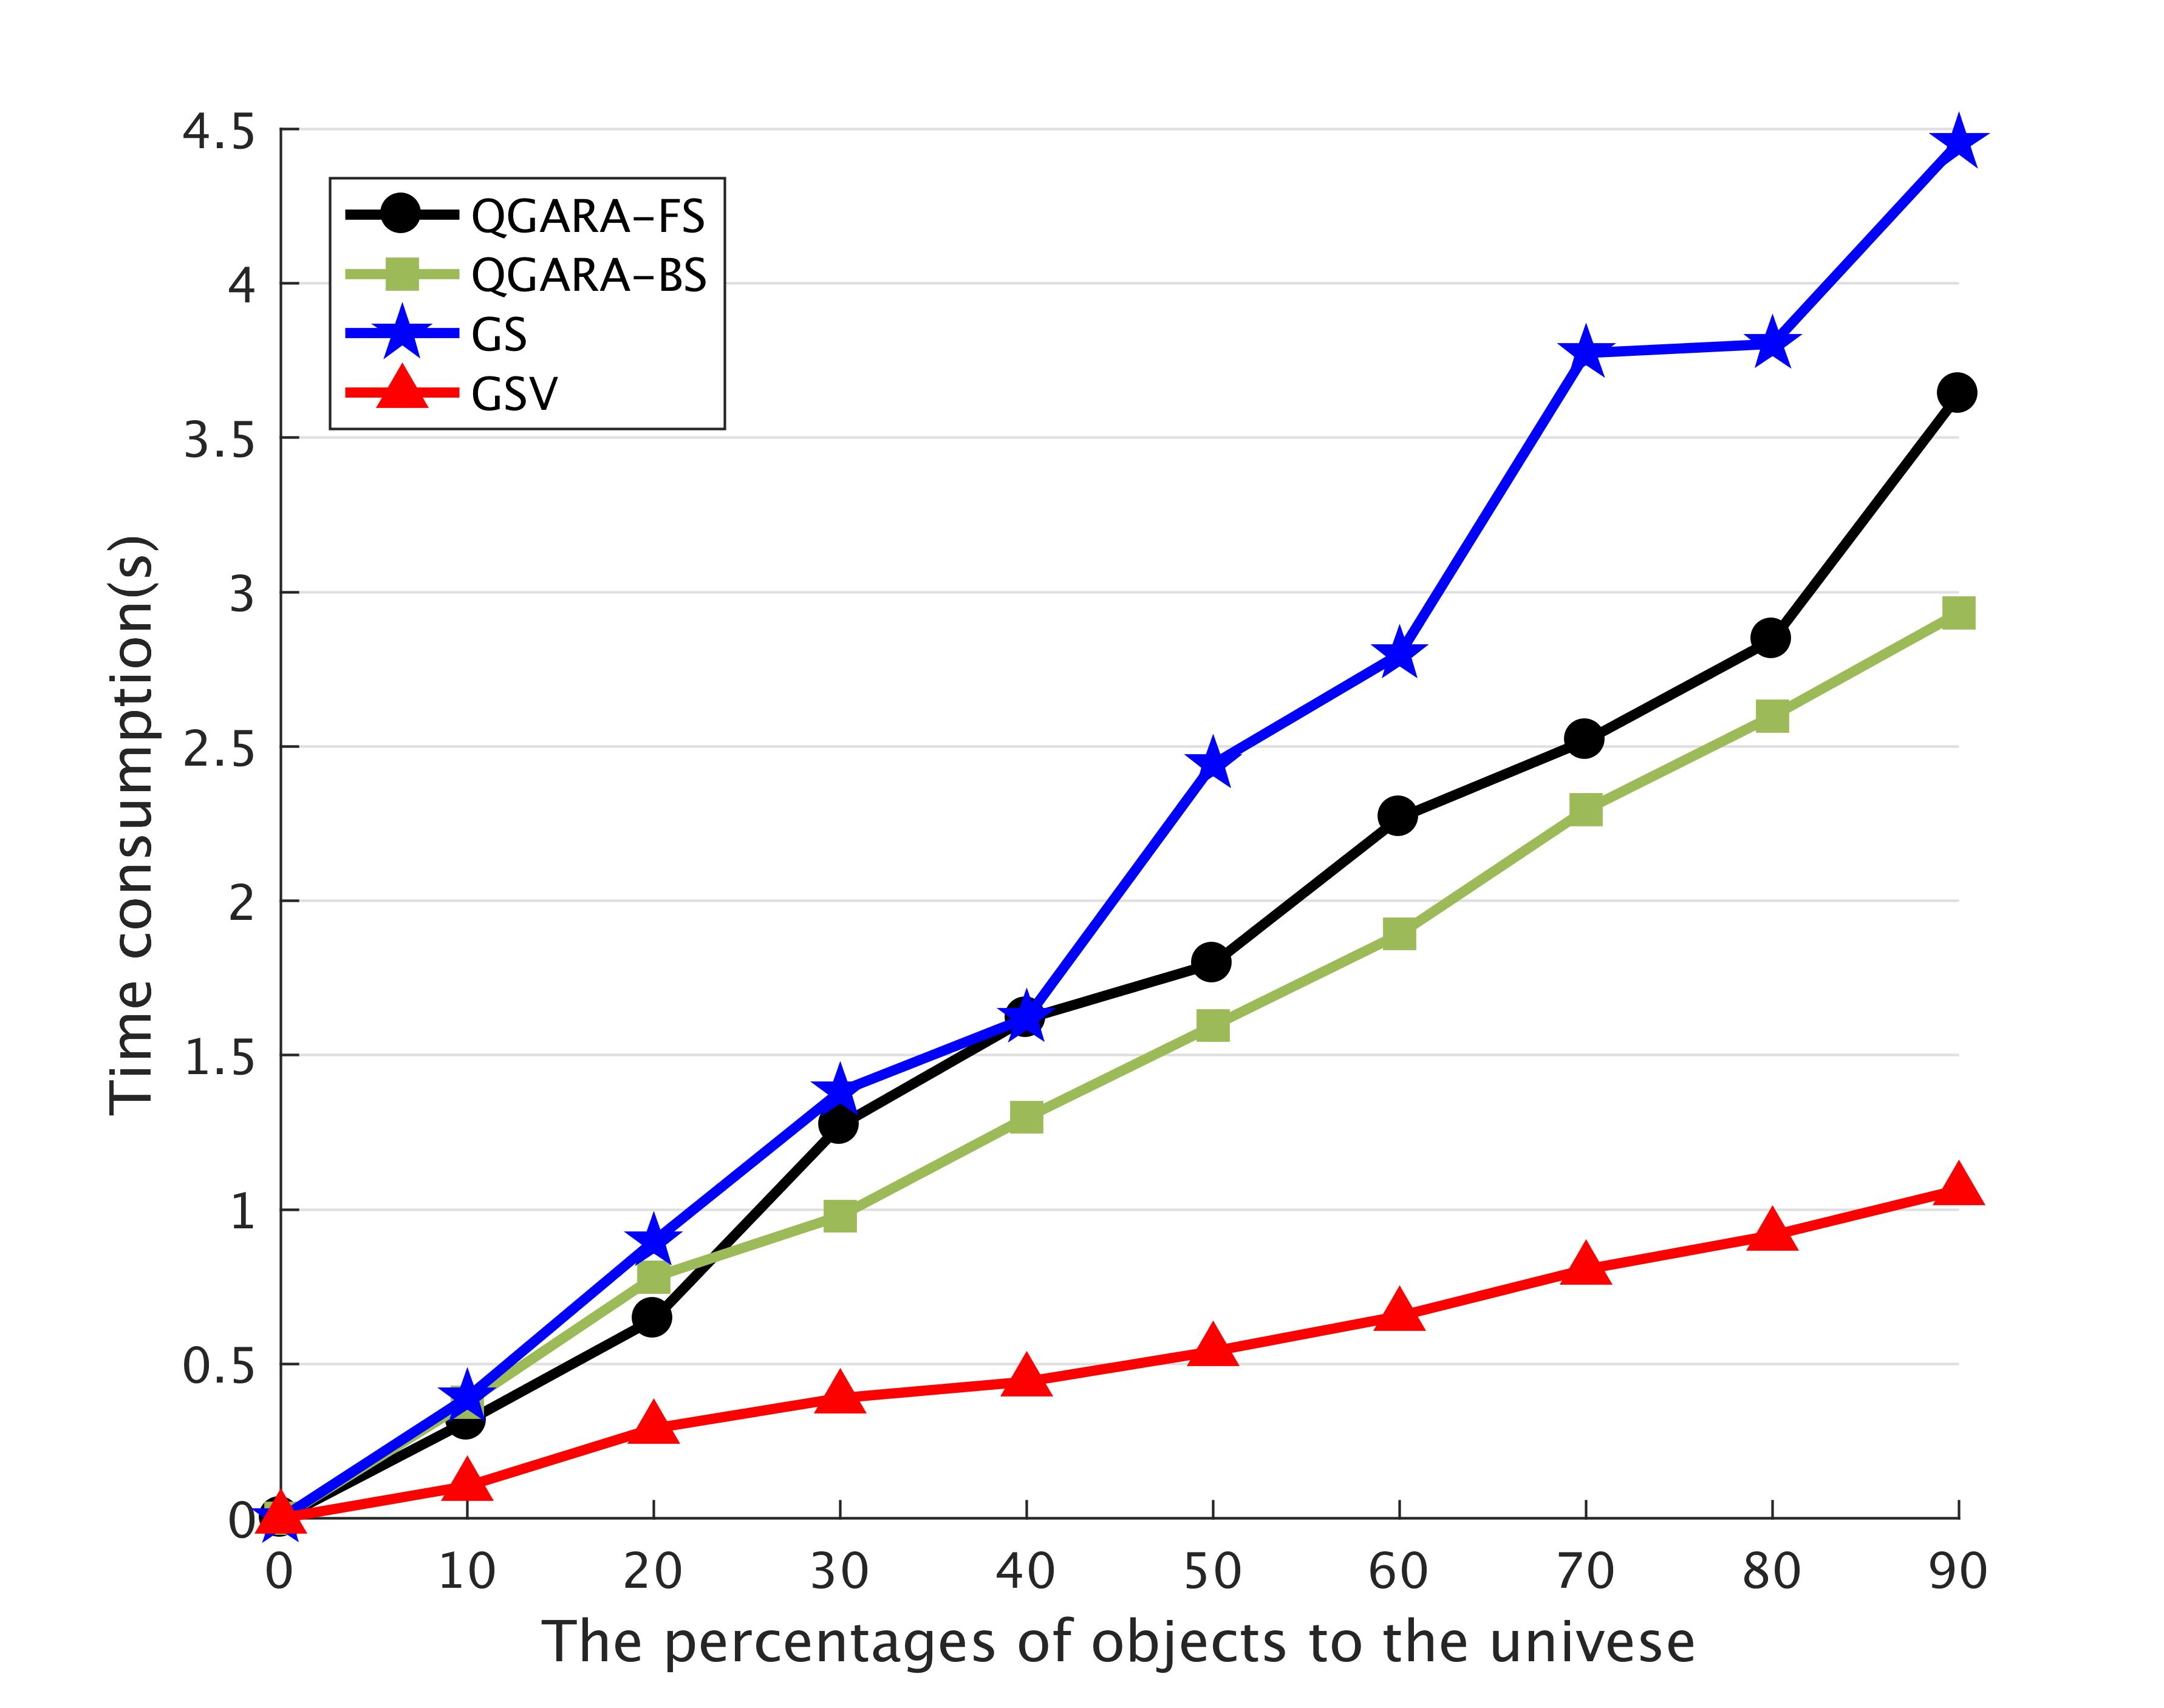
\includegraphics[width=5cm]{./Curve_universe/1.jpg} 
%			}
			\subfigure[Mushroom]{
				\label{Fig.sub1.2}
				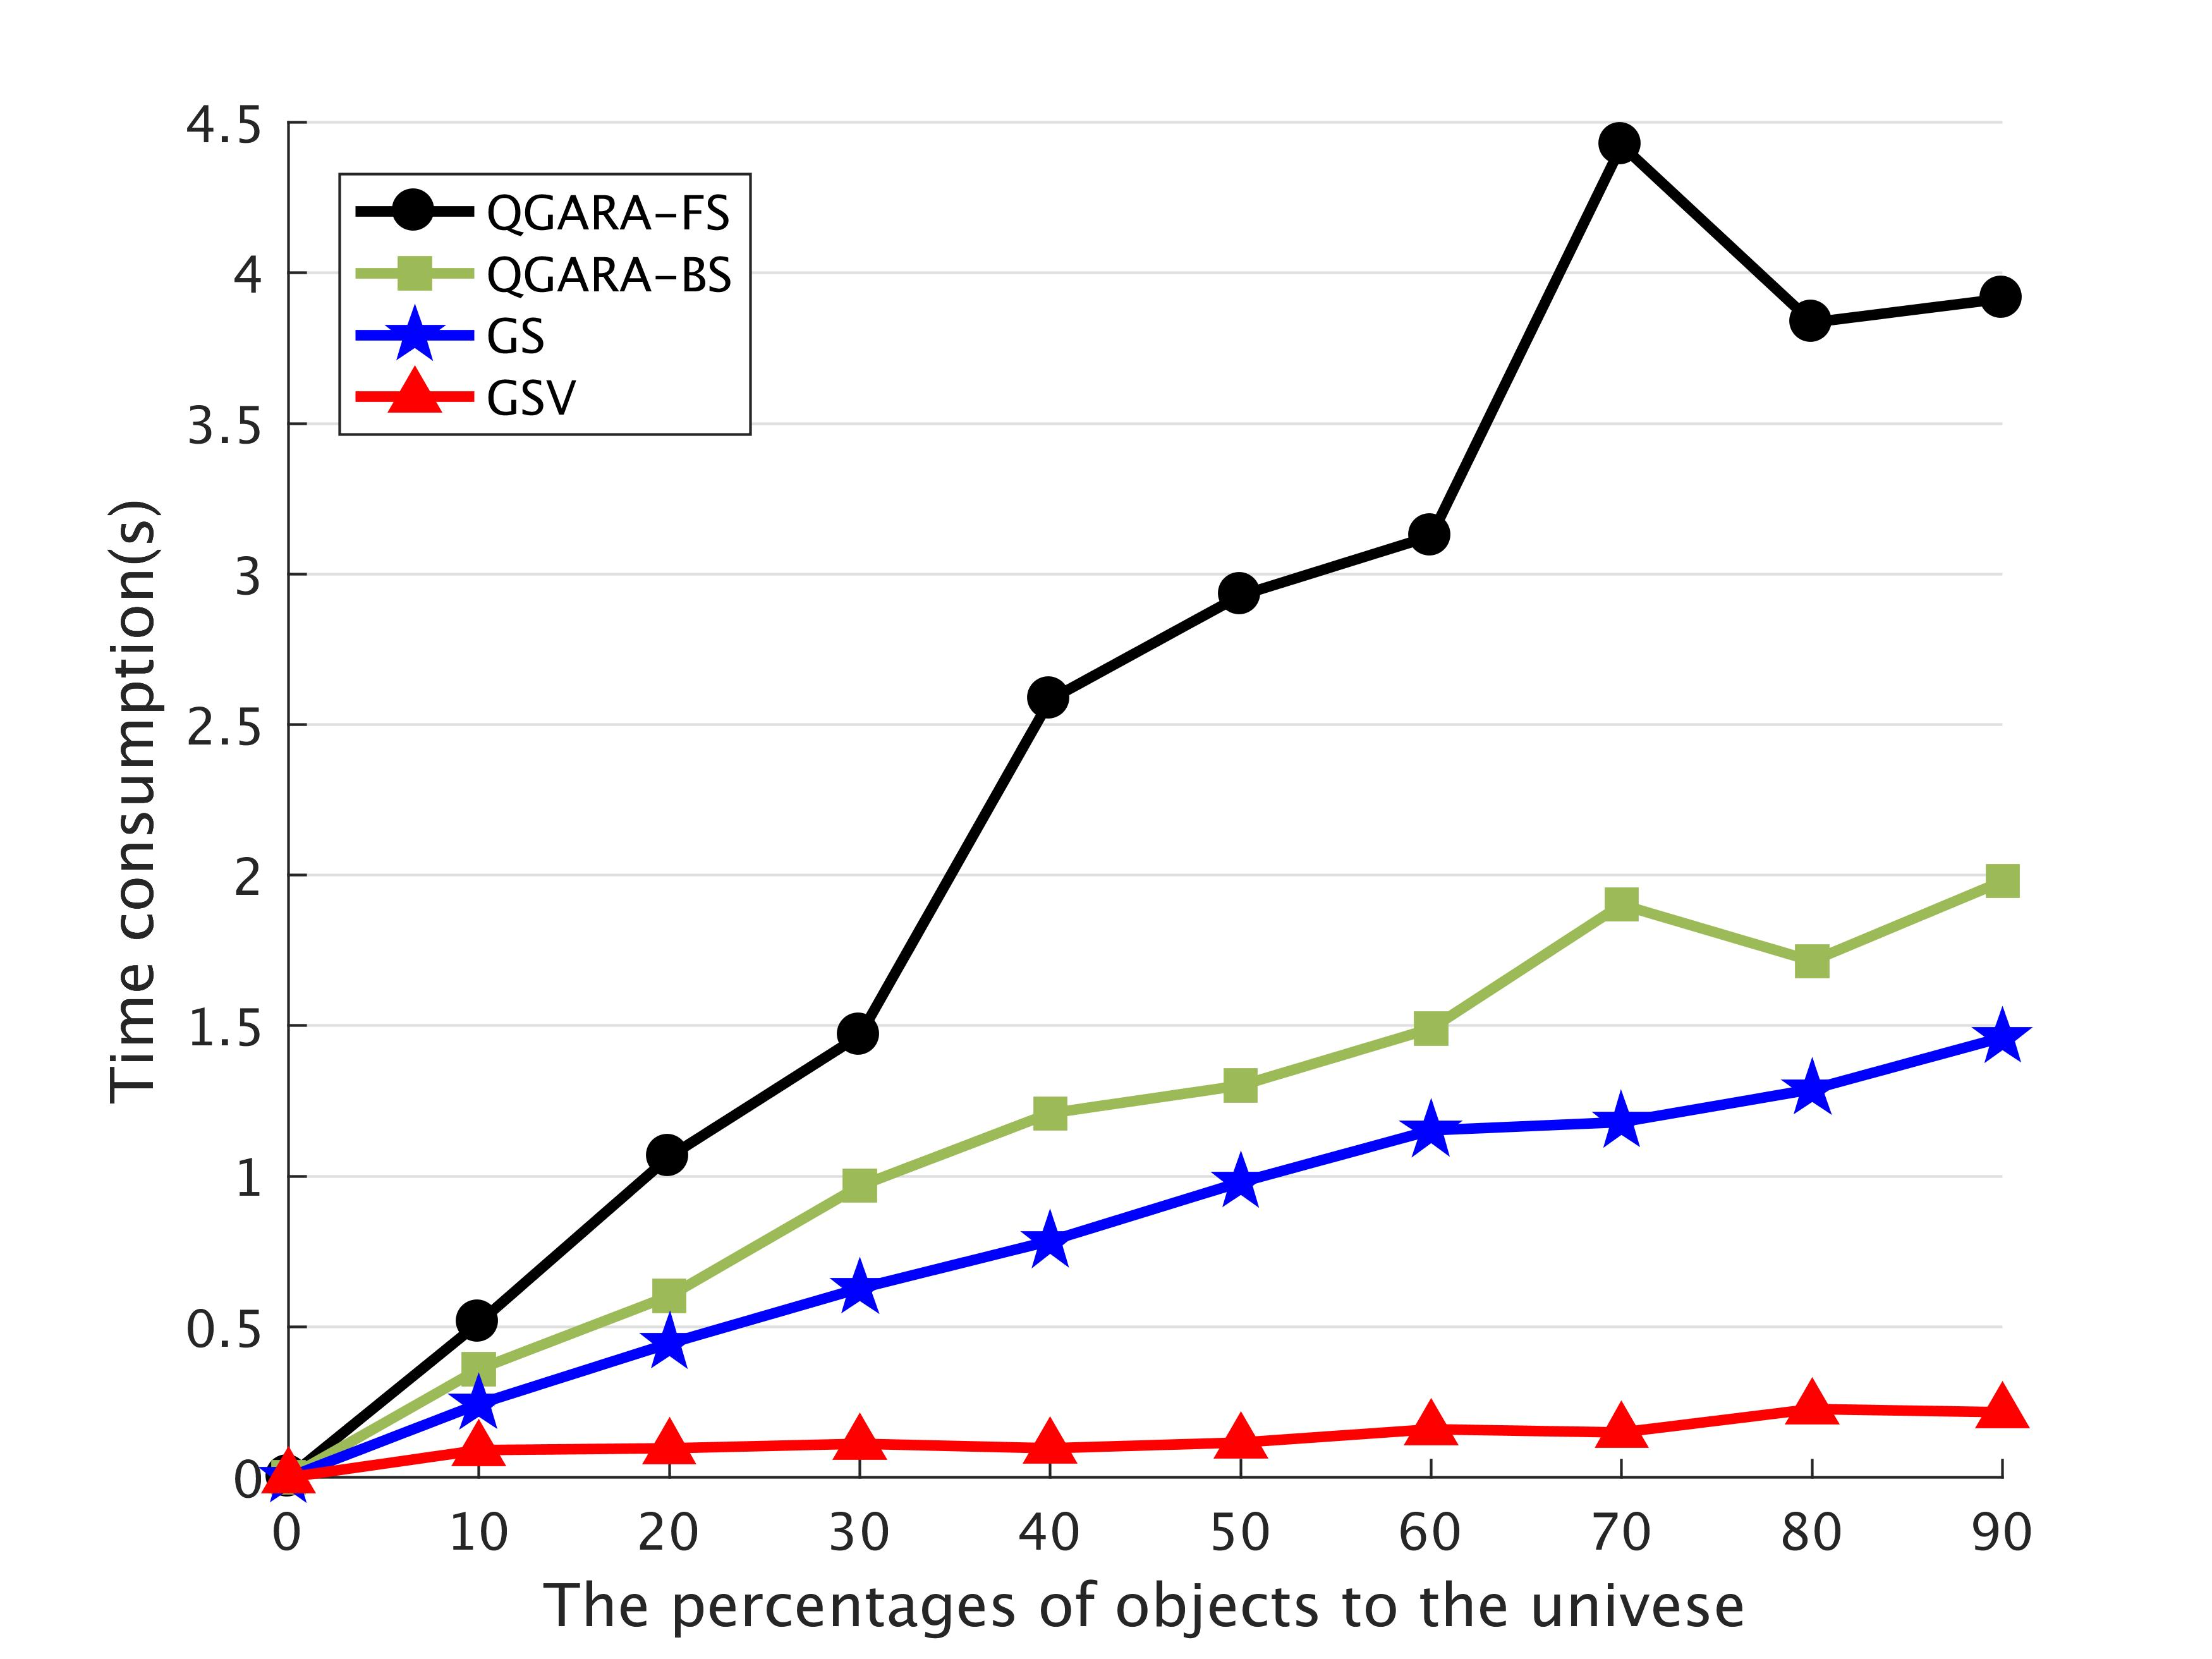
\includegraphics[width=5cm]{./Curve_universe/1_mushroom_pos.jpg} 
			}
			\subfigure[Tic]{
				\label{Fig.sub1.3}
				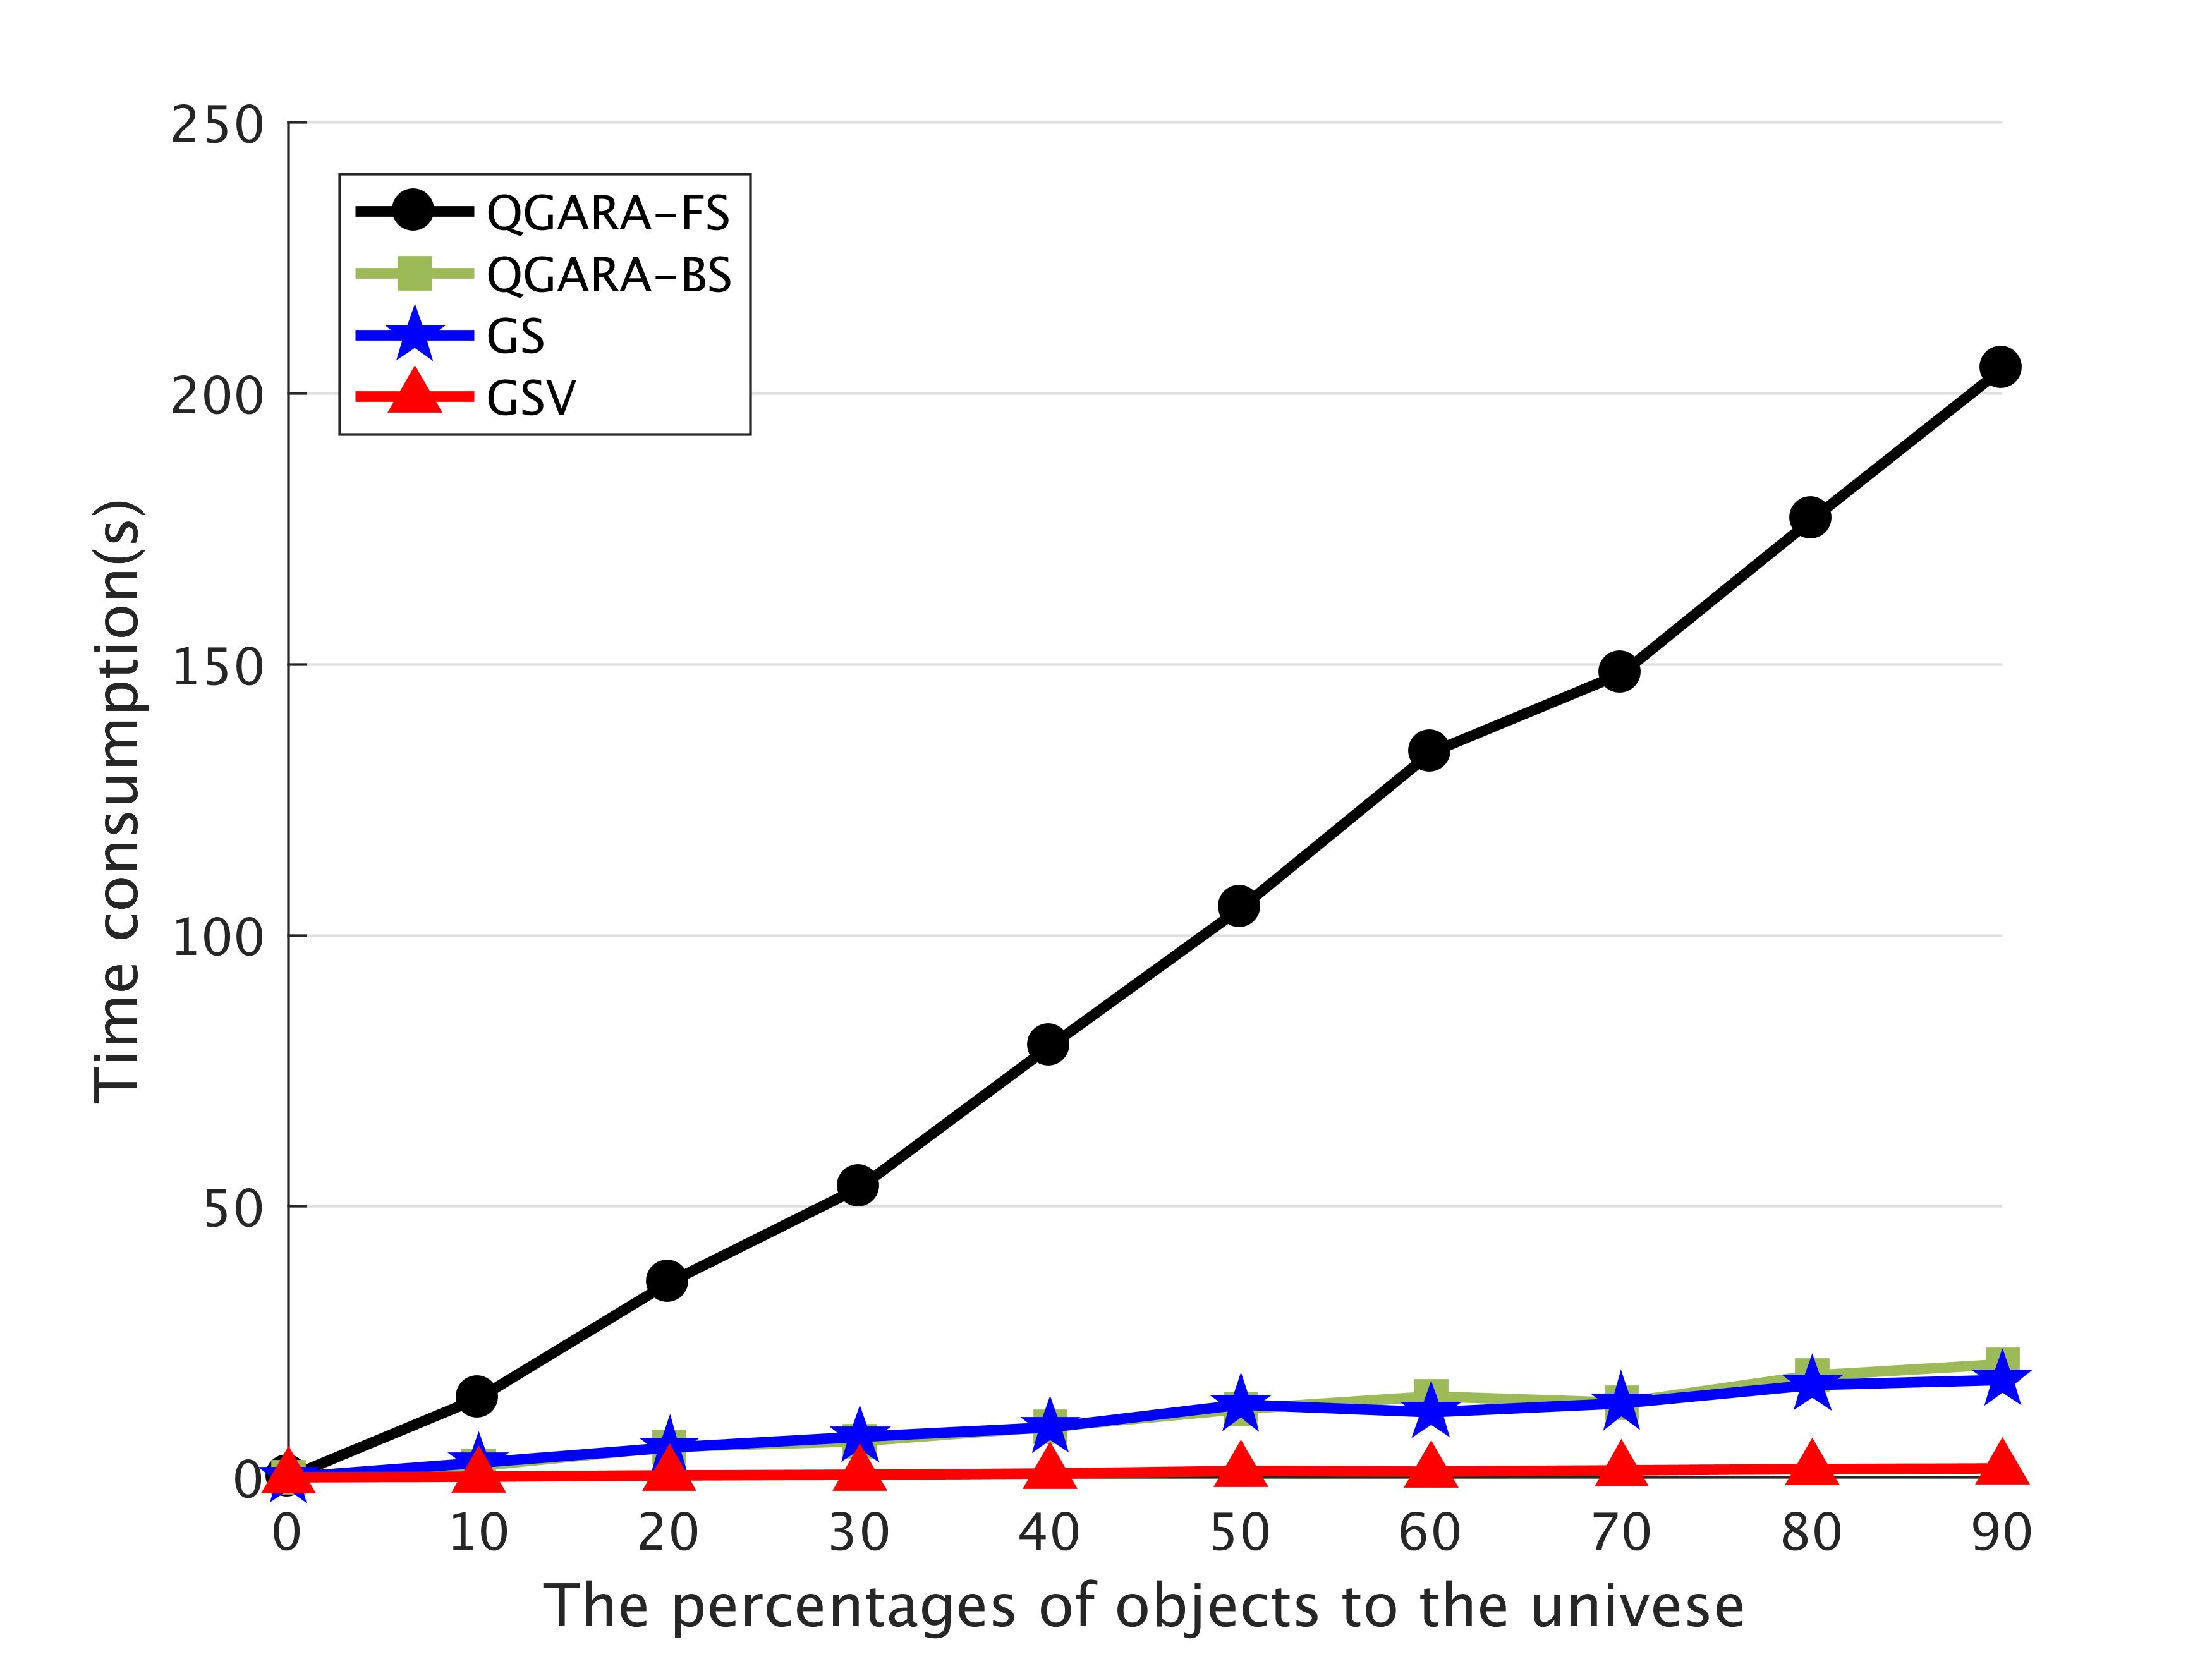
\includegraphics[width=5cm]{./Curve_universe/2_tic_pos.jpg} 
			}
%			\subfigure[Segmentation]{
%				\label{Fig.sub1.4}
%				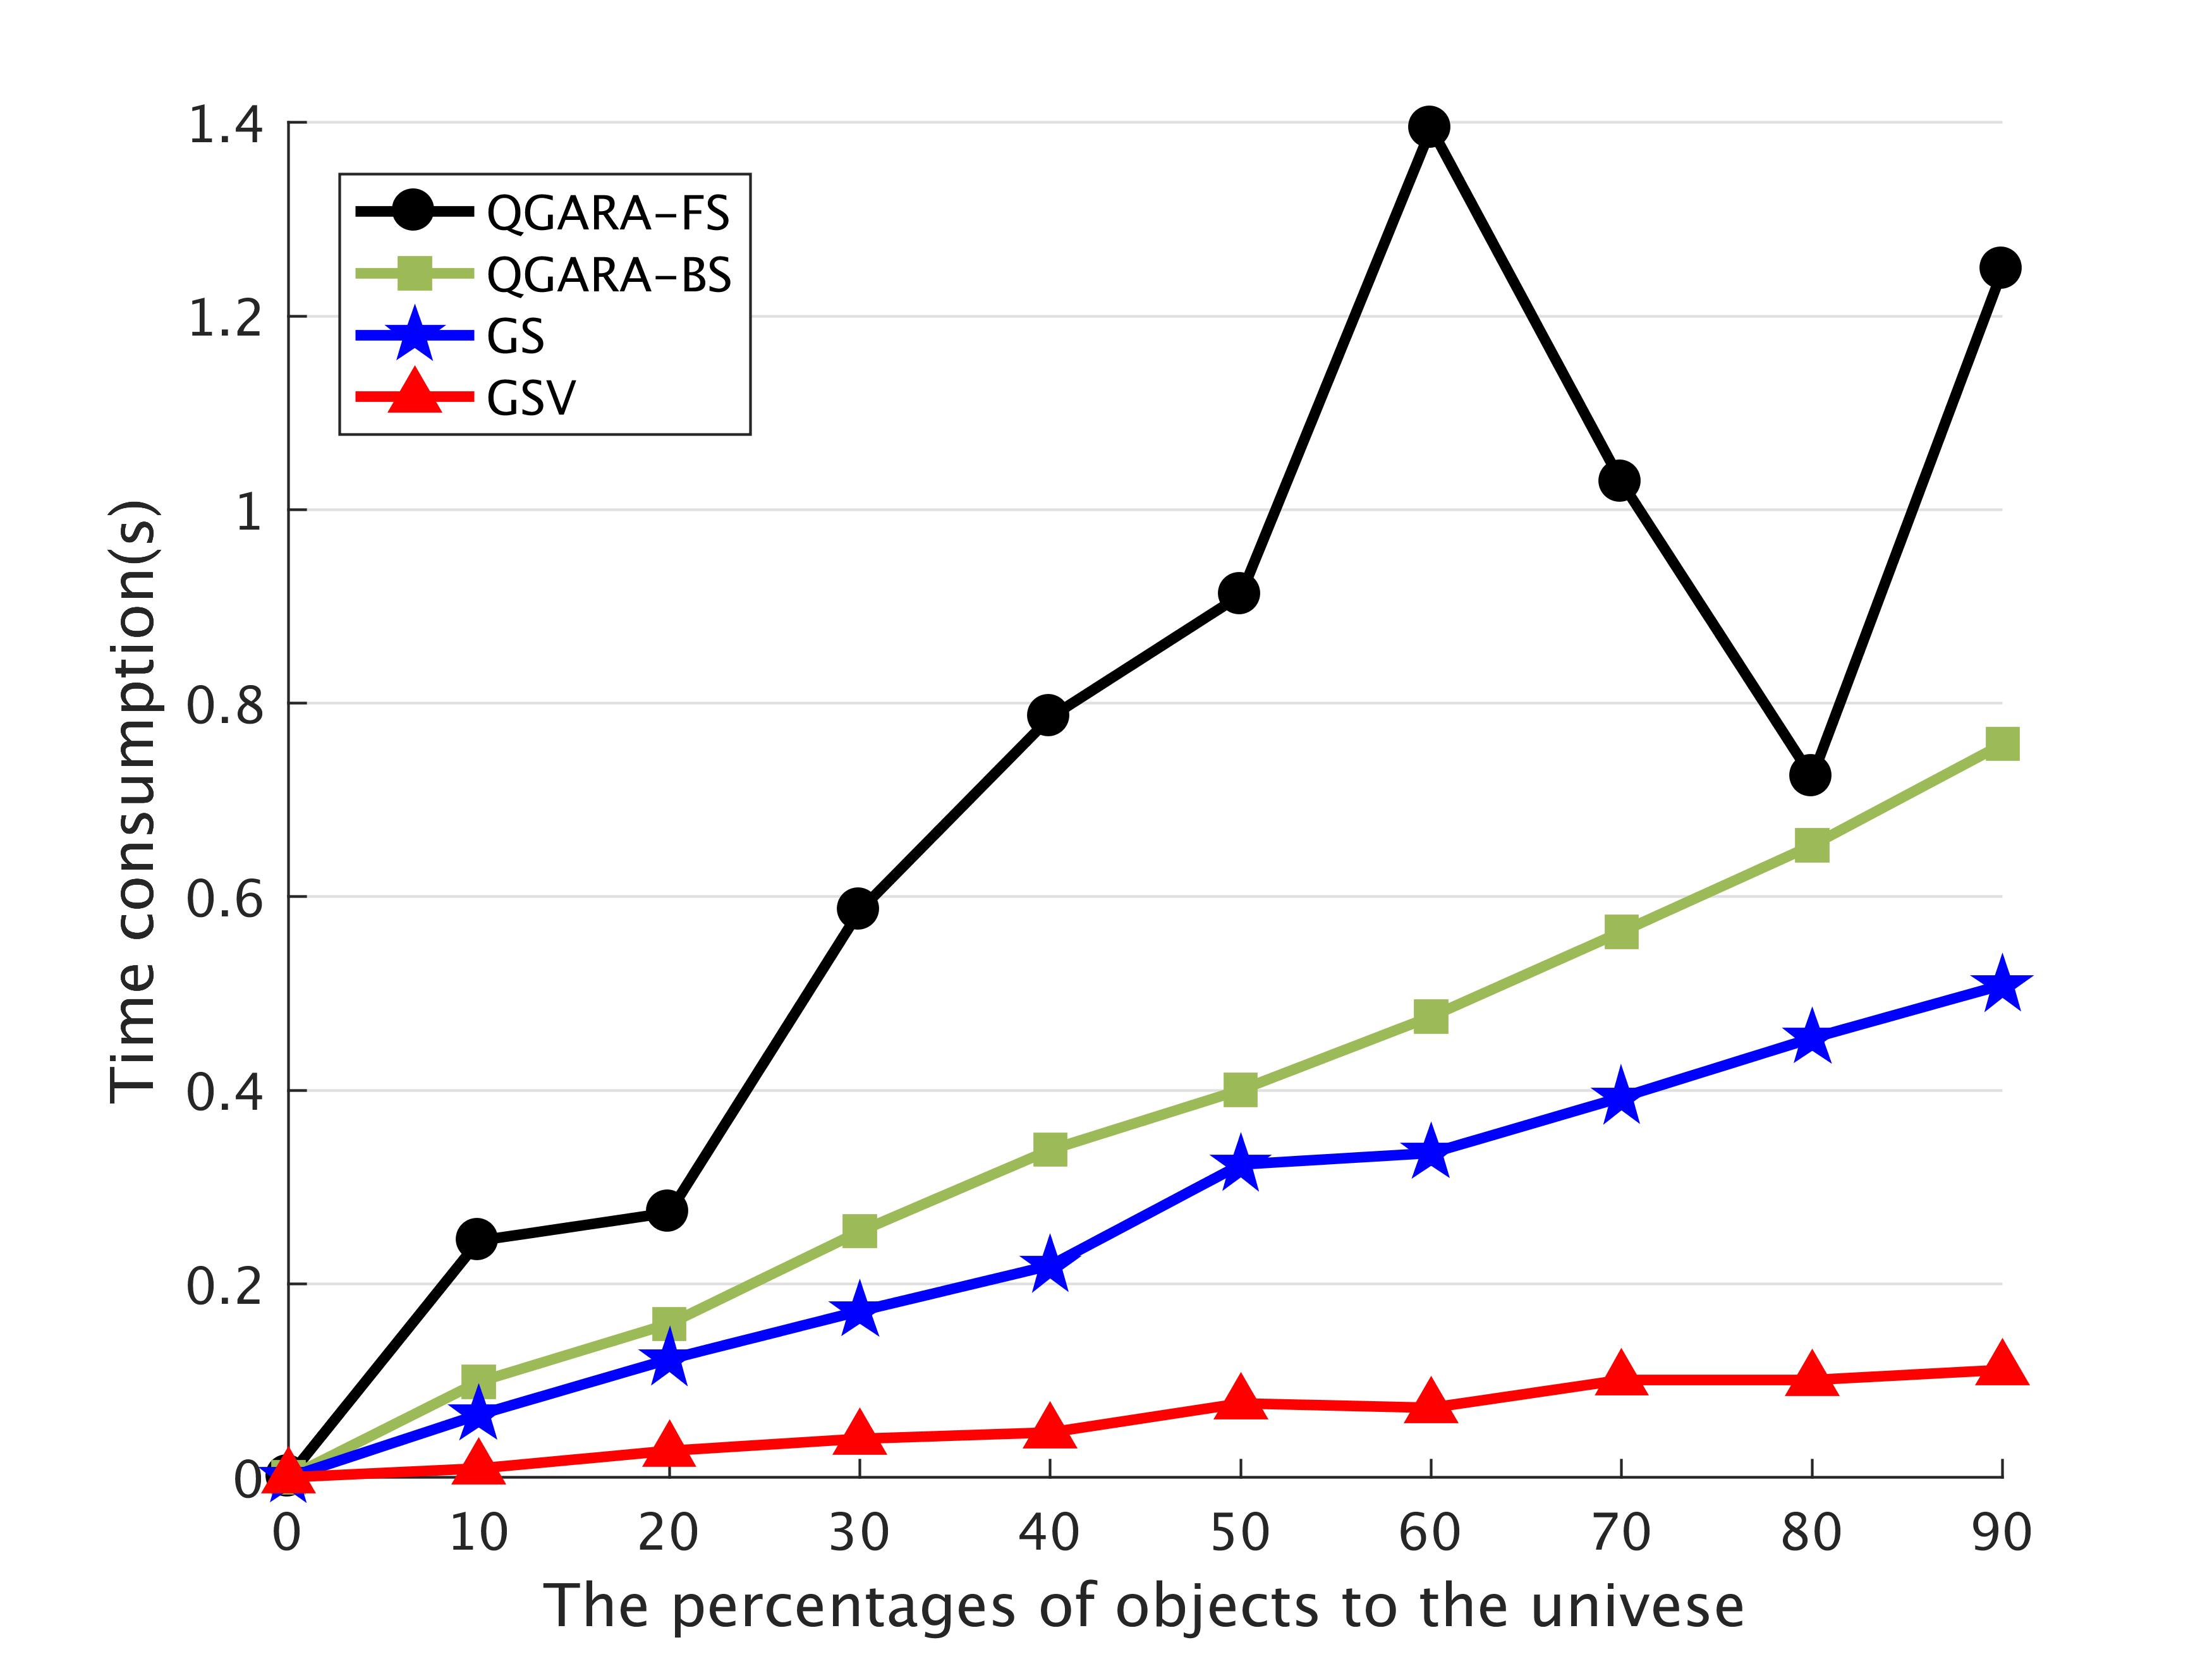
\includegraphics[width=5cm]{./Curve_universe/3_seg_pos.jpg} 
%			}
	%		\subfigure[pid(int)]{
	%			\label{Fig.sub1.5}
	%			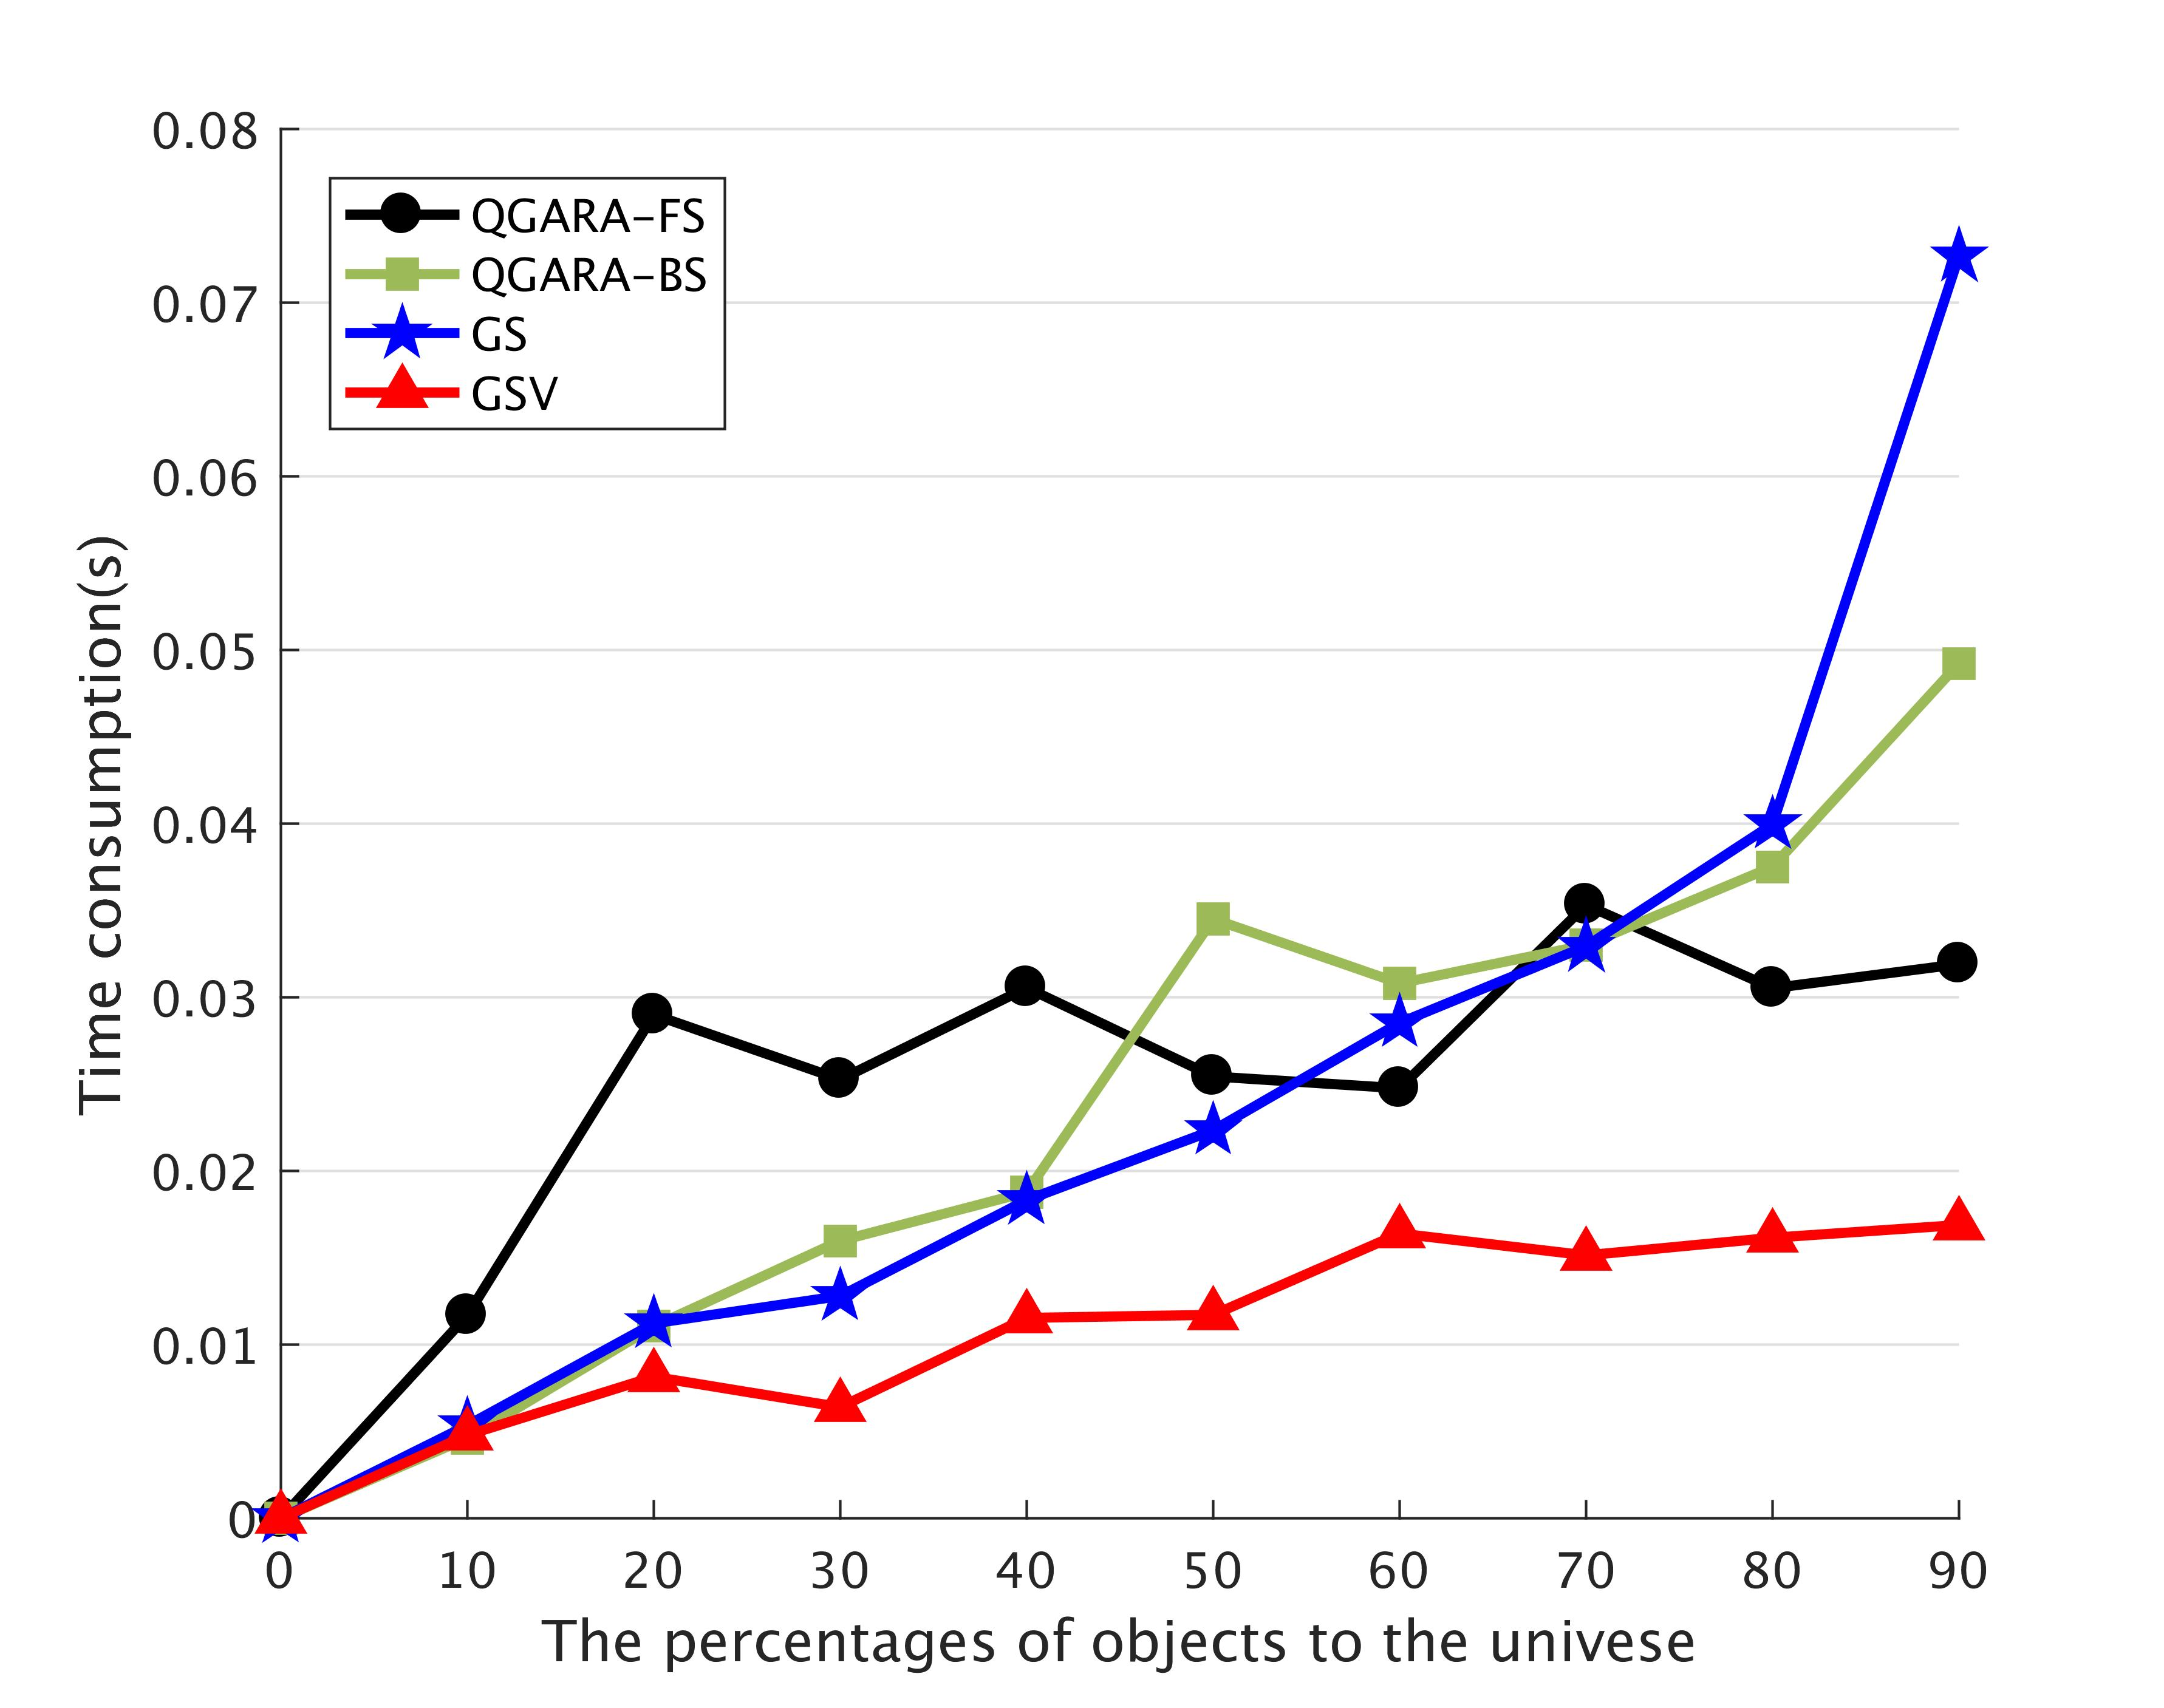
\includegraphics[width=5cm]{./Curve_universe/5.jpg} 
	%		}
			\subfigure[Splice]{
				\label{Fig.sub1.6}
				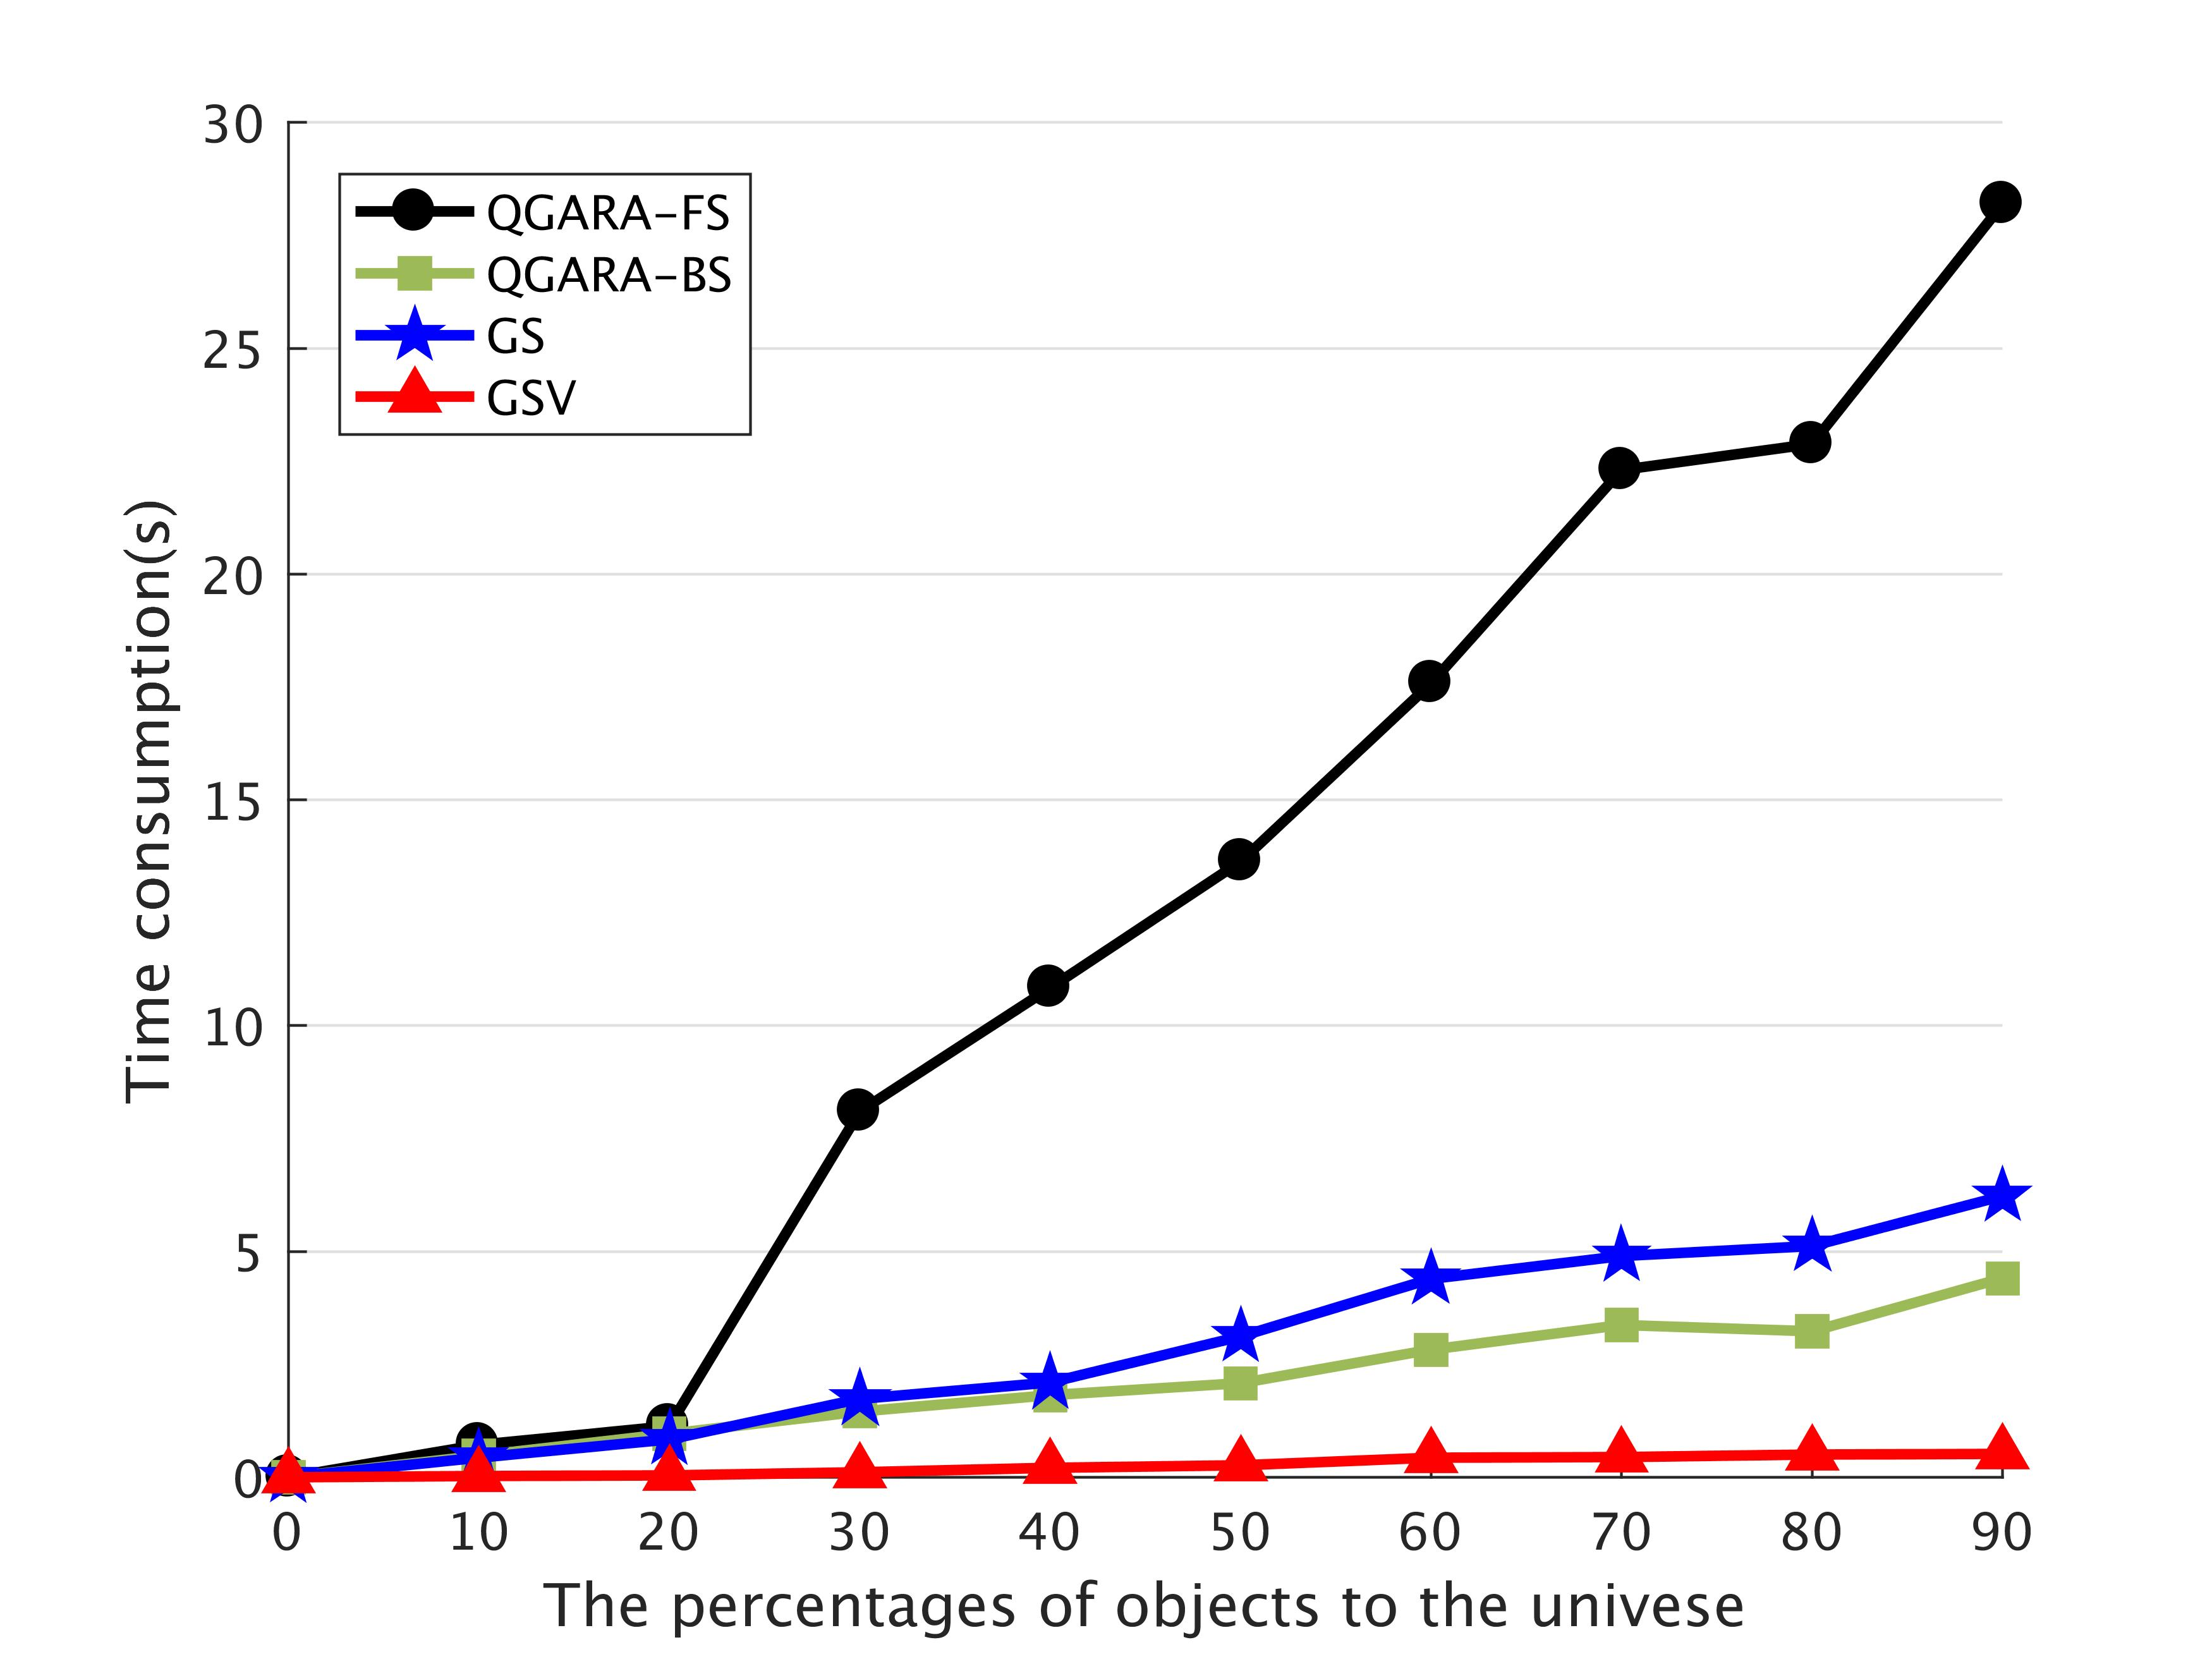
\includegraphics[width=5cm]{./Curve_universe/4_splice_pos.jpg} 
			}
			\subfigure[Dermatology]{
				\label{Fig.sub1.7}
				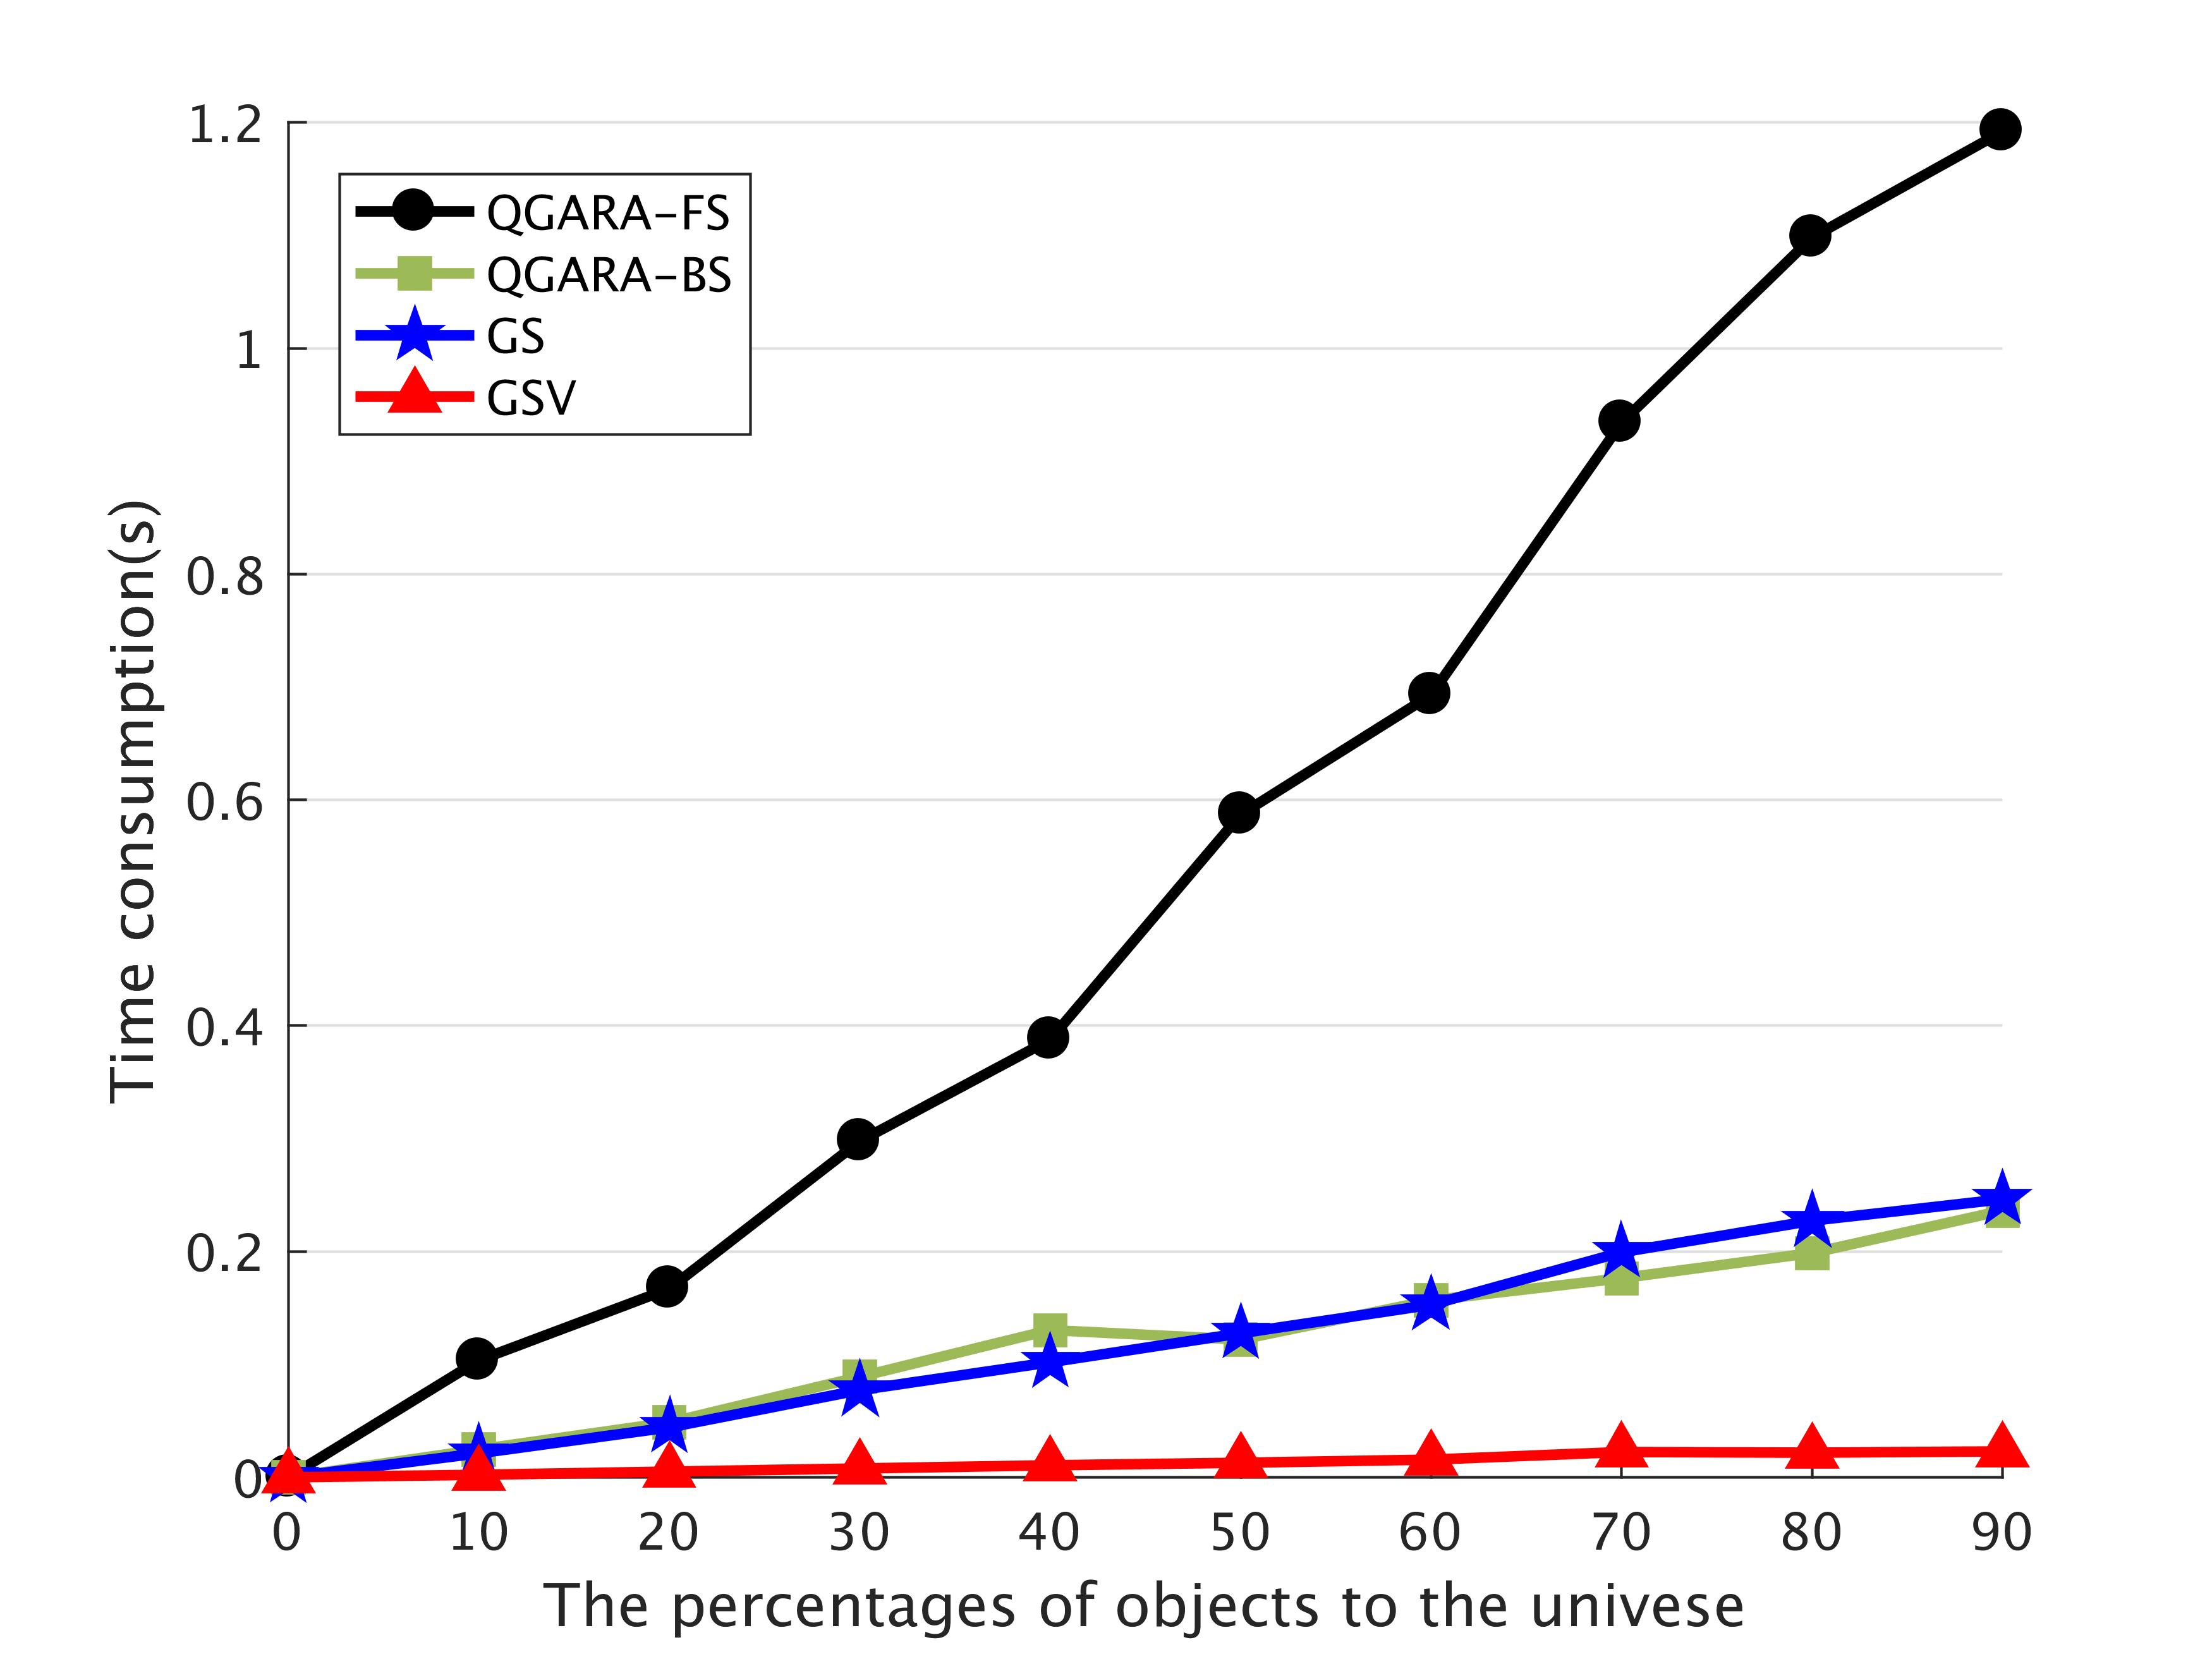
\includegraphics[width=5cm]{./Curve_universe/5_dermatology_pos.jpg} 
			}
			\subfigure[Wdbc]{
				\label{Fig.sub1.8}
				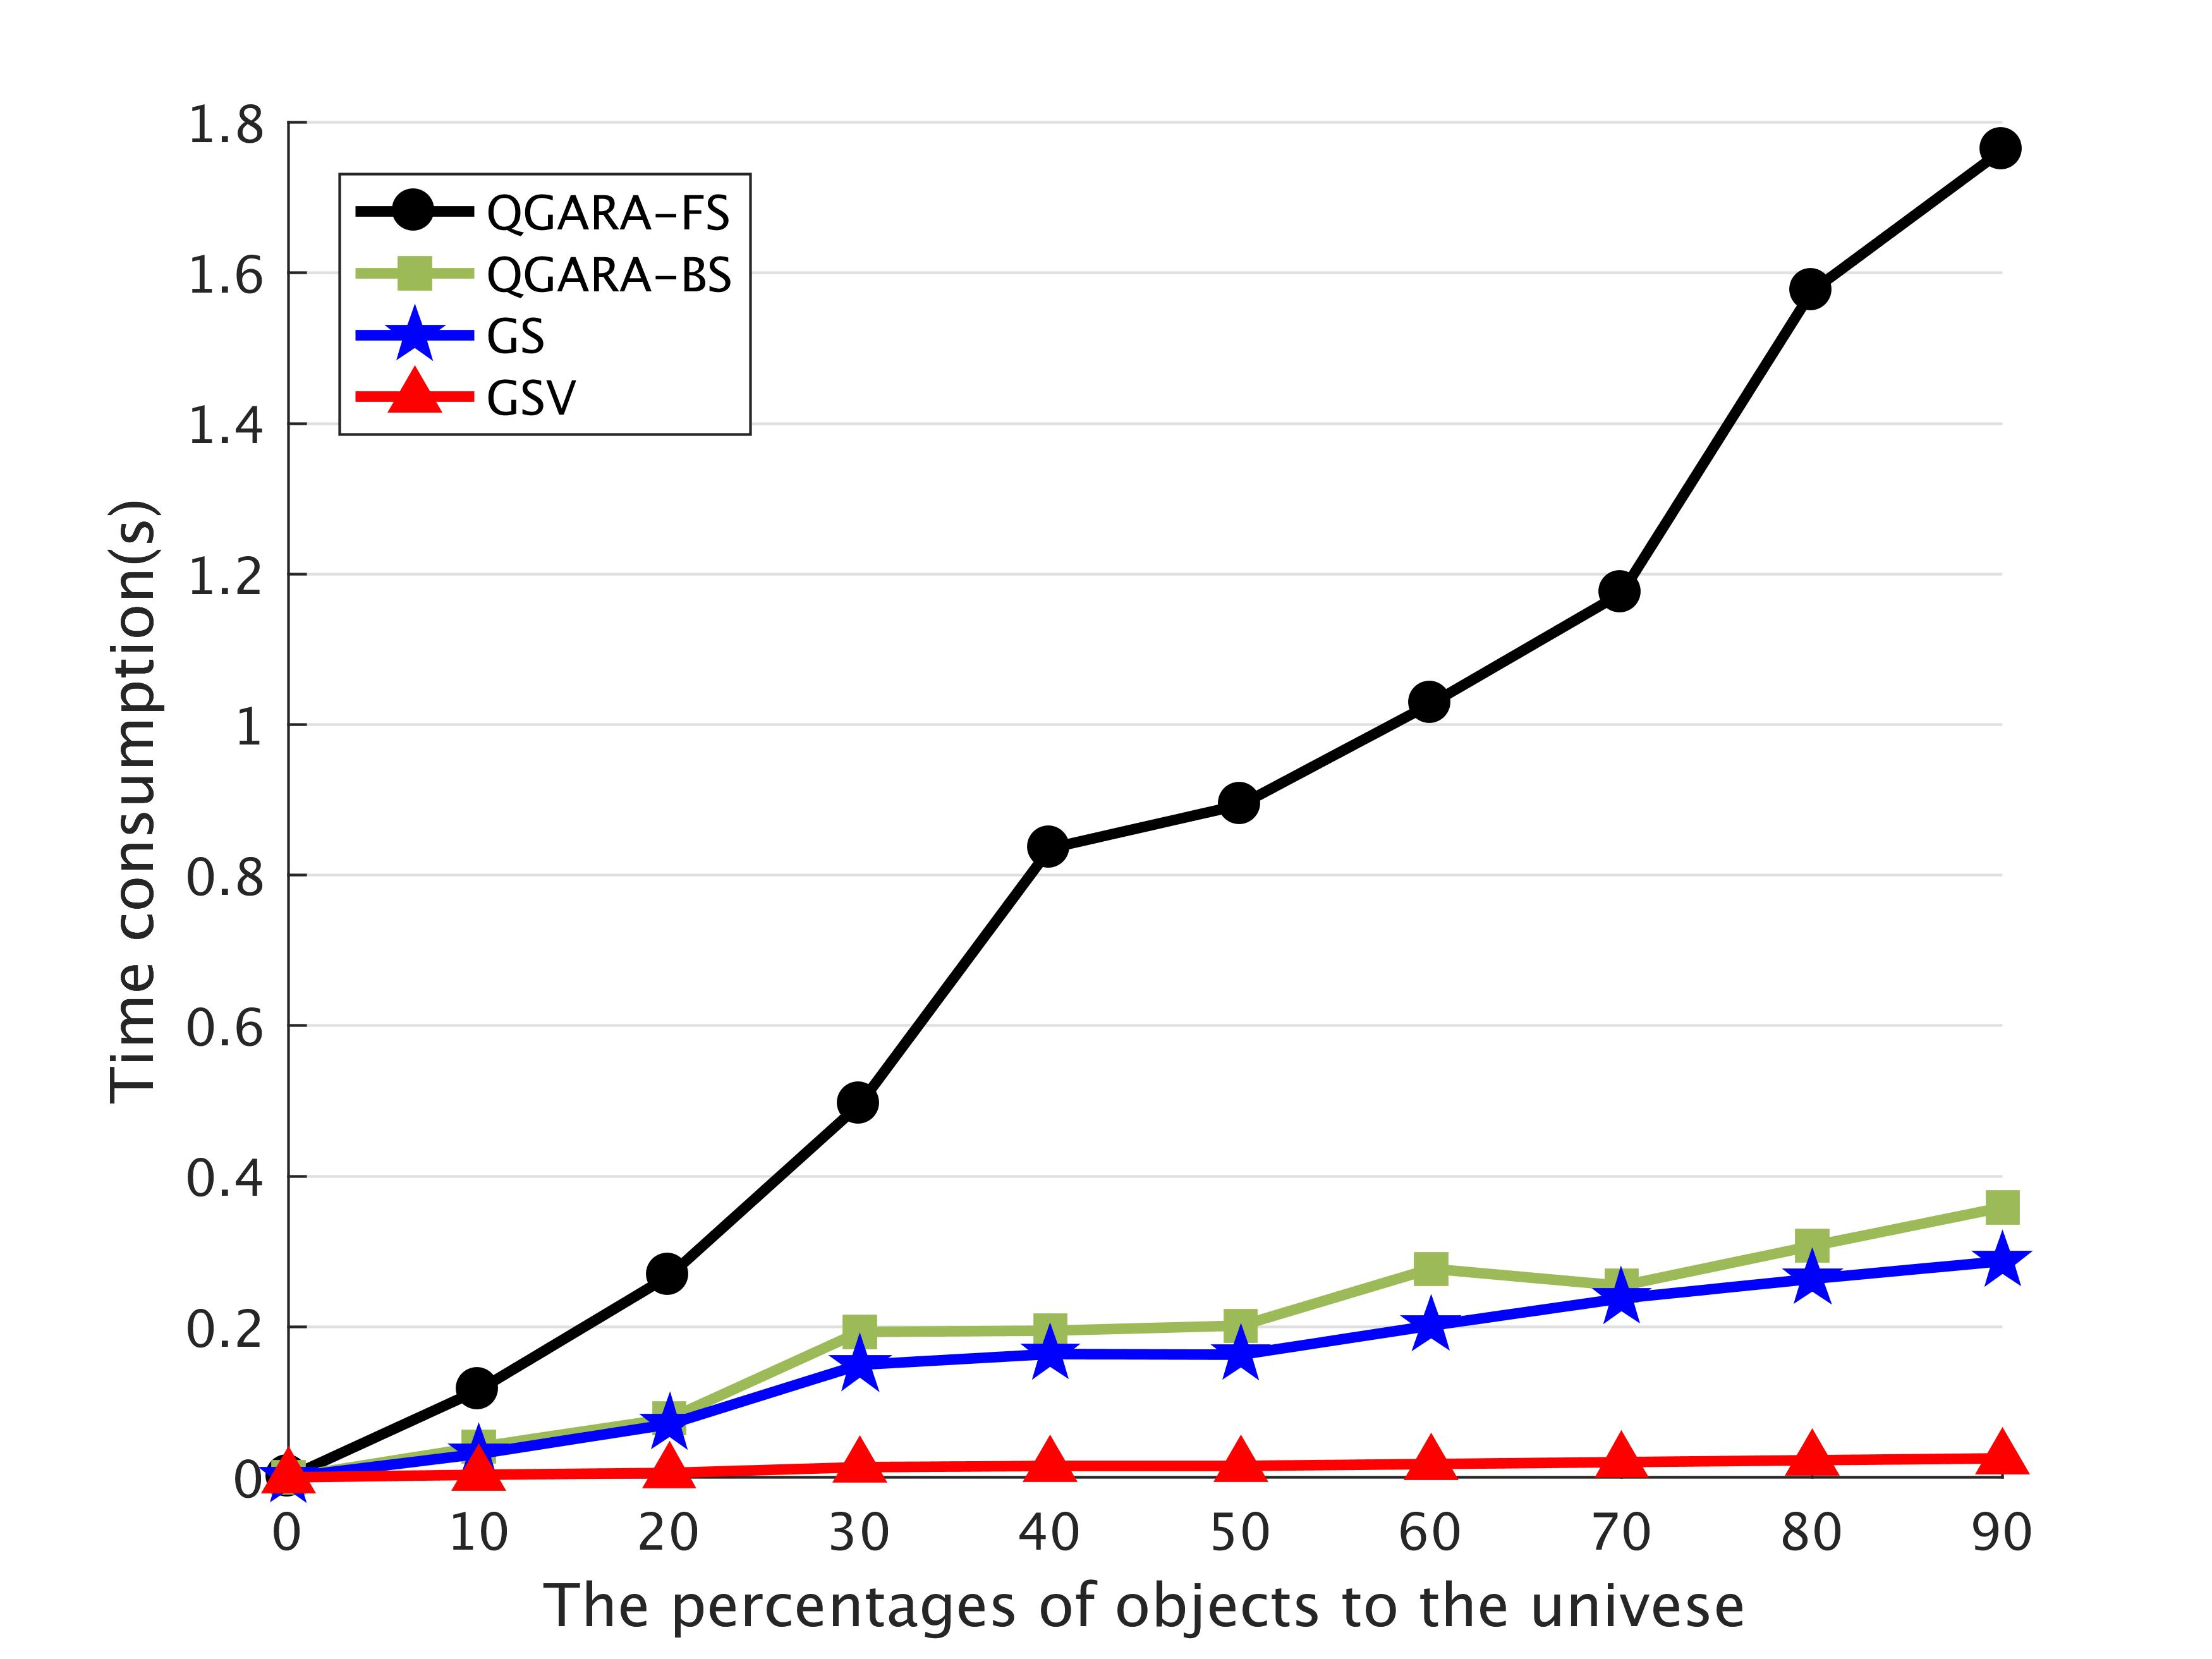
\includegraphics[width=5cm]{./Curve_universe/6_wdbc_pos.jpg} 
			}
	%	\end{figure}
	%	\begin{figure}[htbp]
			\subfigure[CNAE9]{
				\label{Fig.sub1.9}
				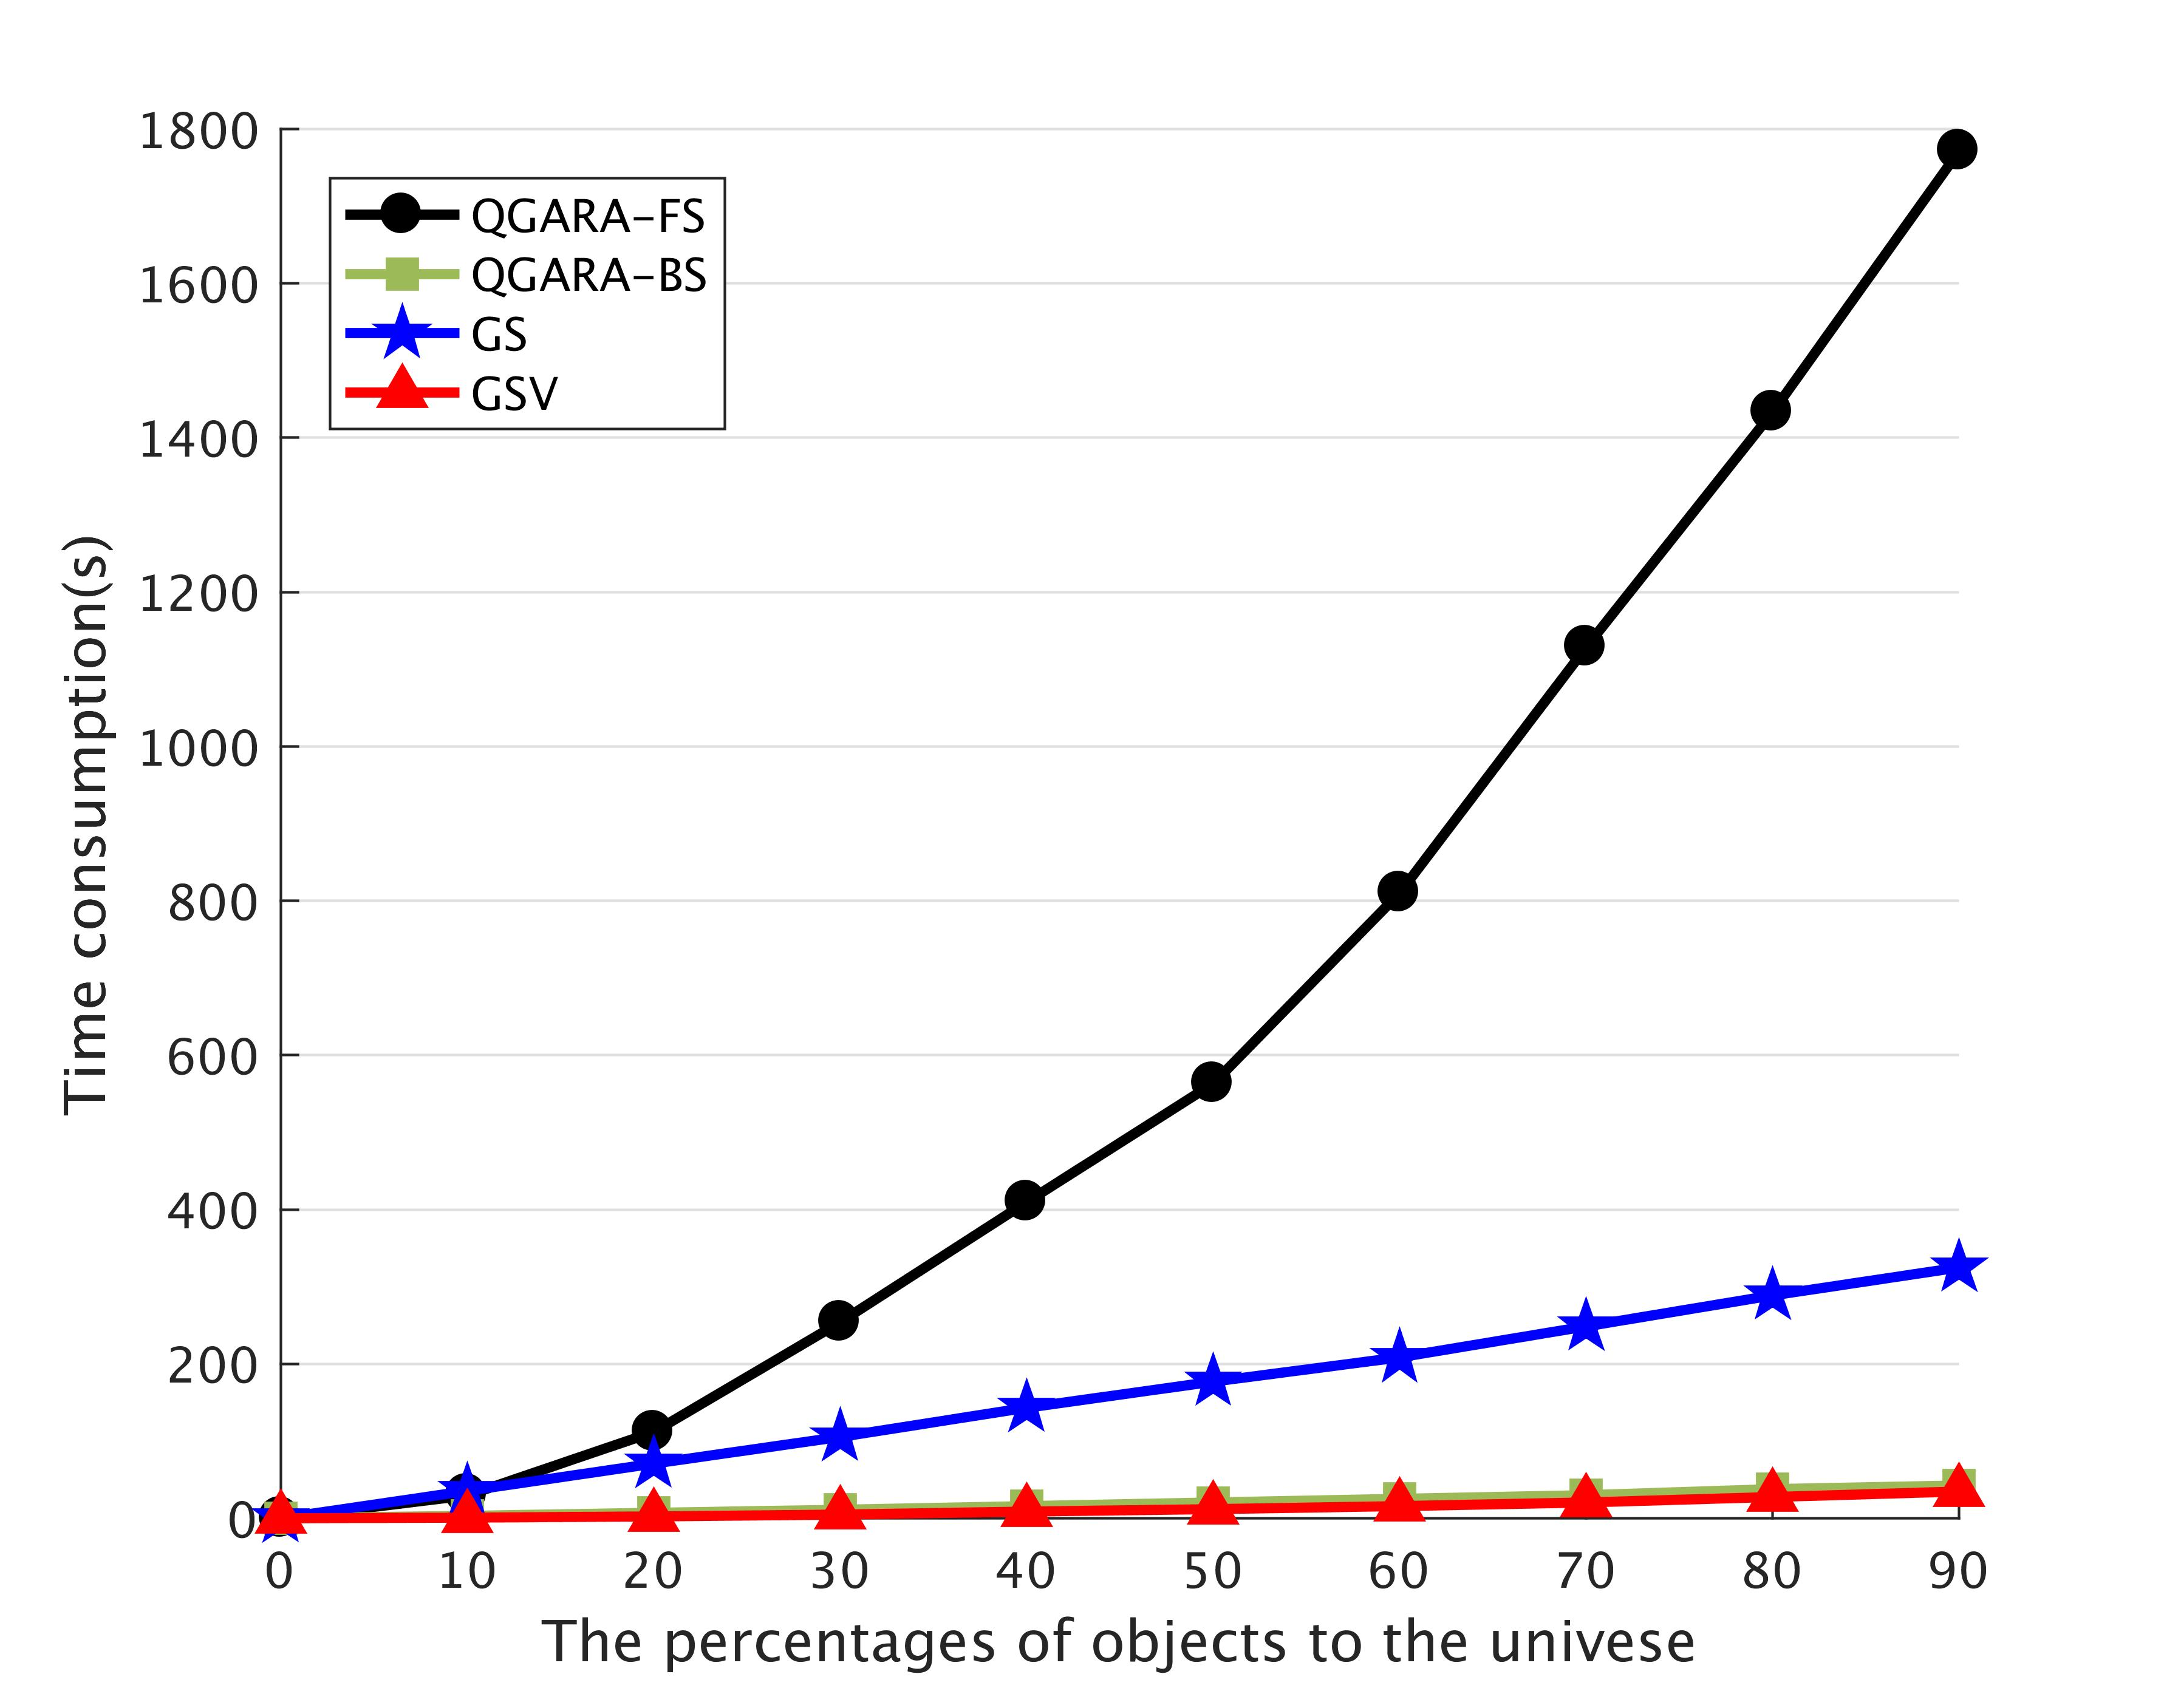
\includegraphics[width=5cm]{./Curve_universe/9.jpg} 
			}
%			\subfigure[Semeion]{
%				\label{Fig.sub1.10}
%				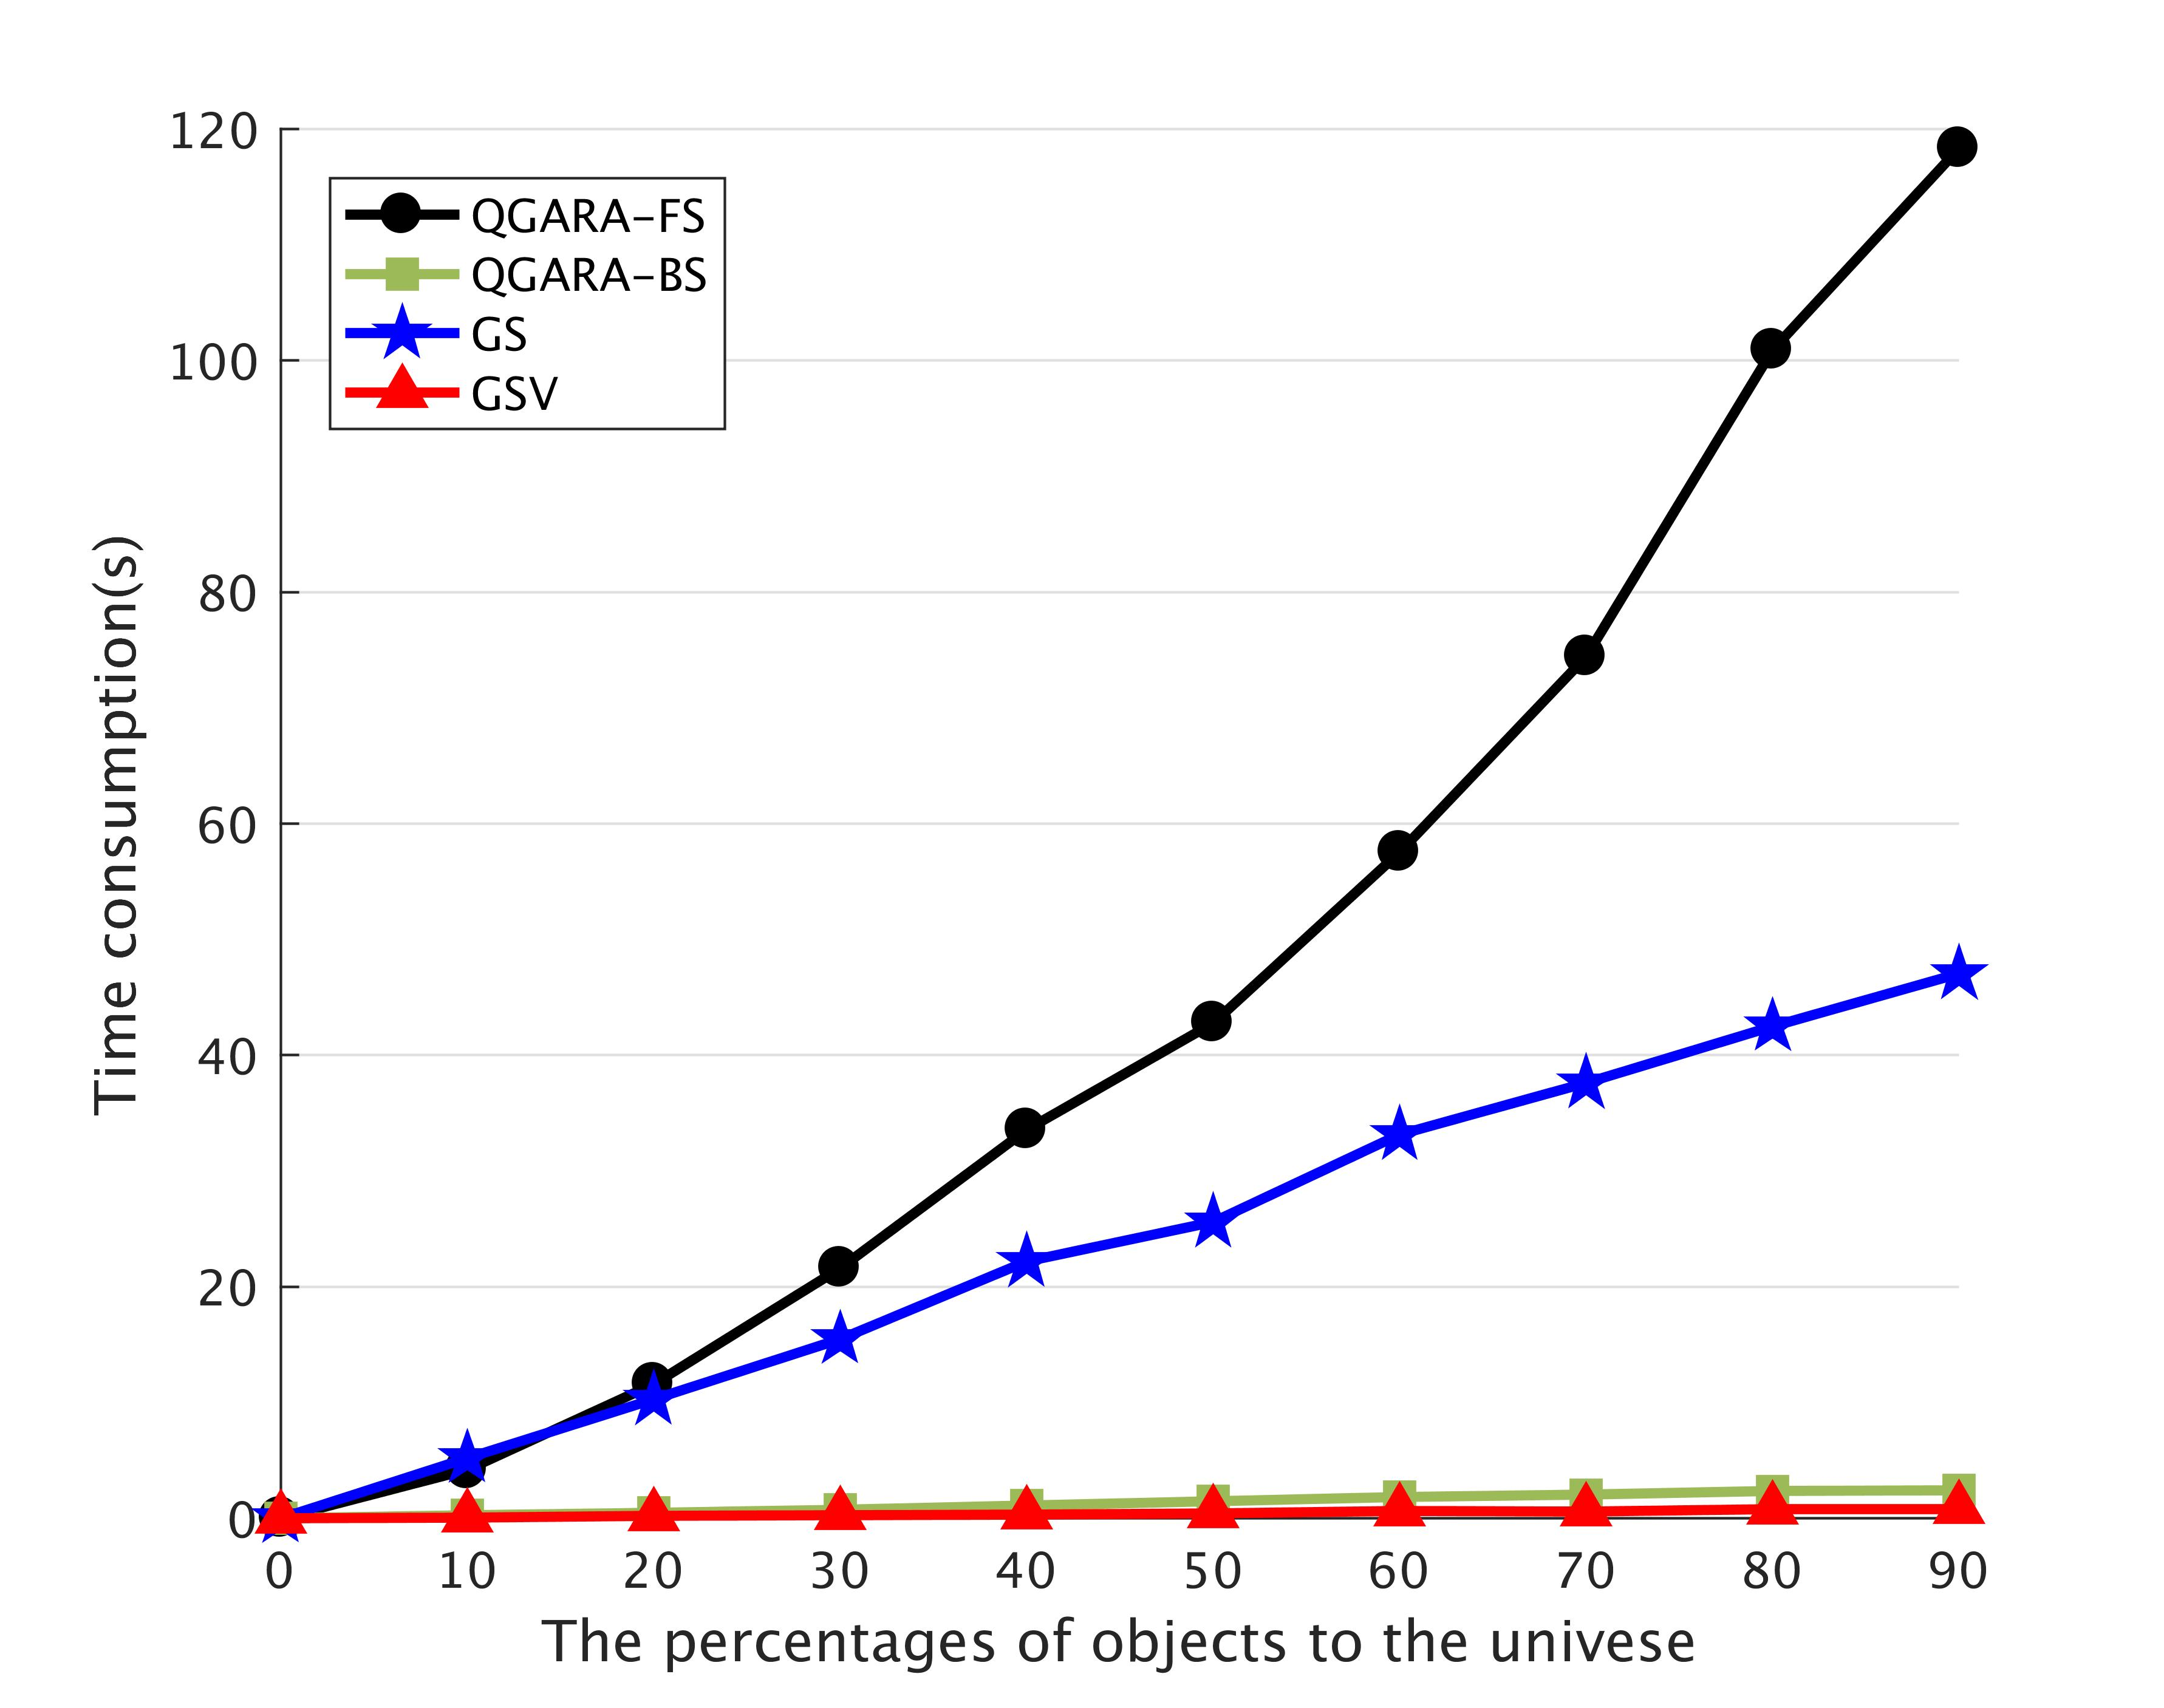
\includegraphics[width=5cm]{./Curve_universe/10.jpg} 
%			}
			\subfigure[DNA]{
				\label{Fig.sub1.11}
				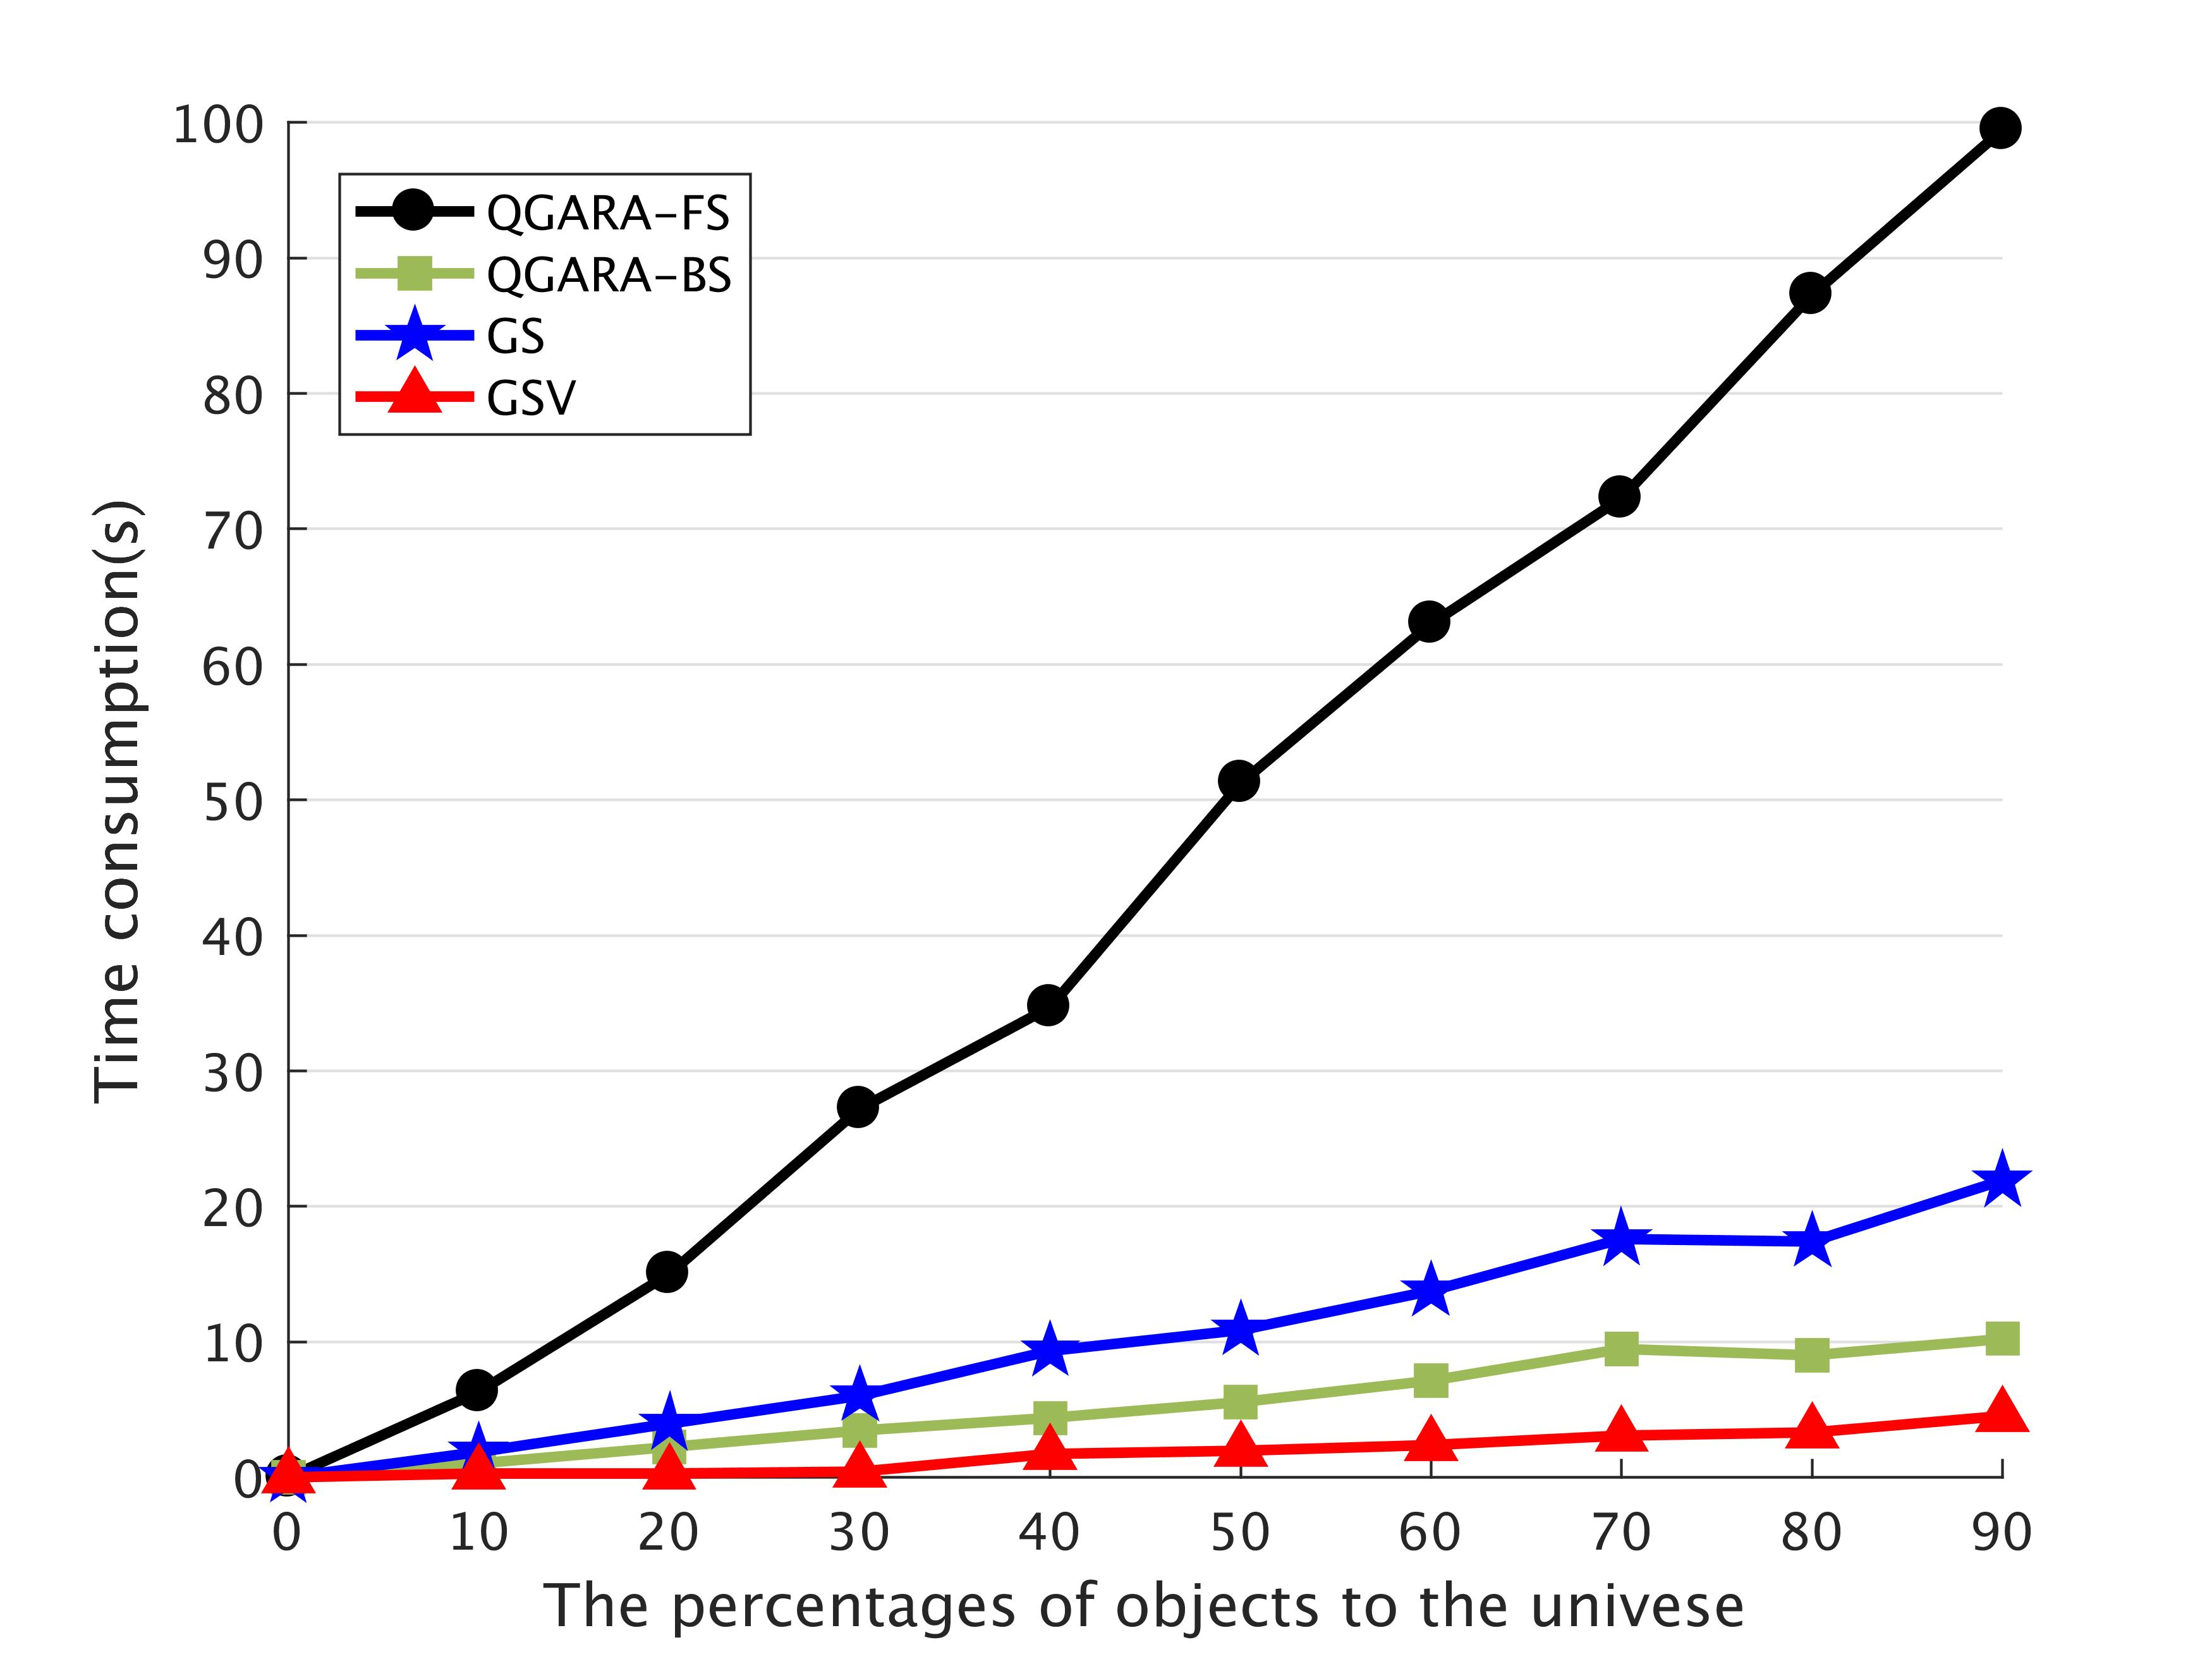
\includegraphics[width=5cm]{./Curve_universe/9_DNA_pos.jpg} 
			}
			\subfigure[Connect4]{
				\label{Fig.sub1.12}
				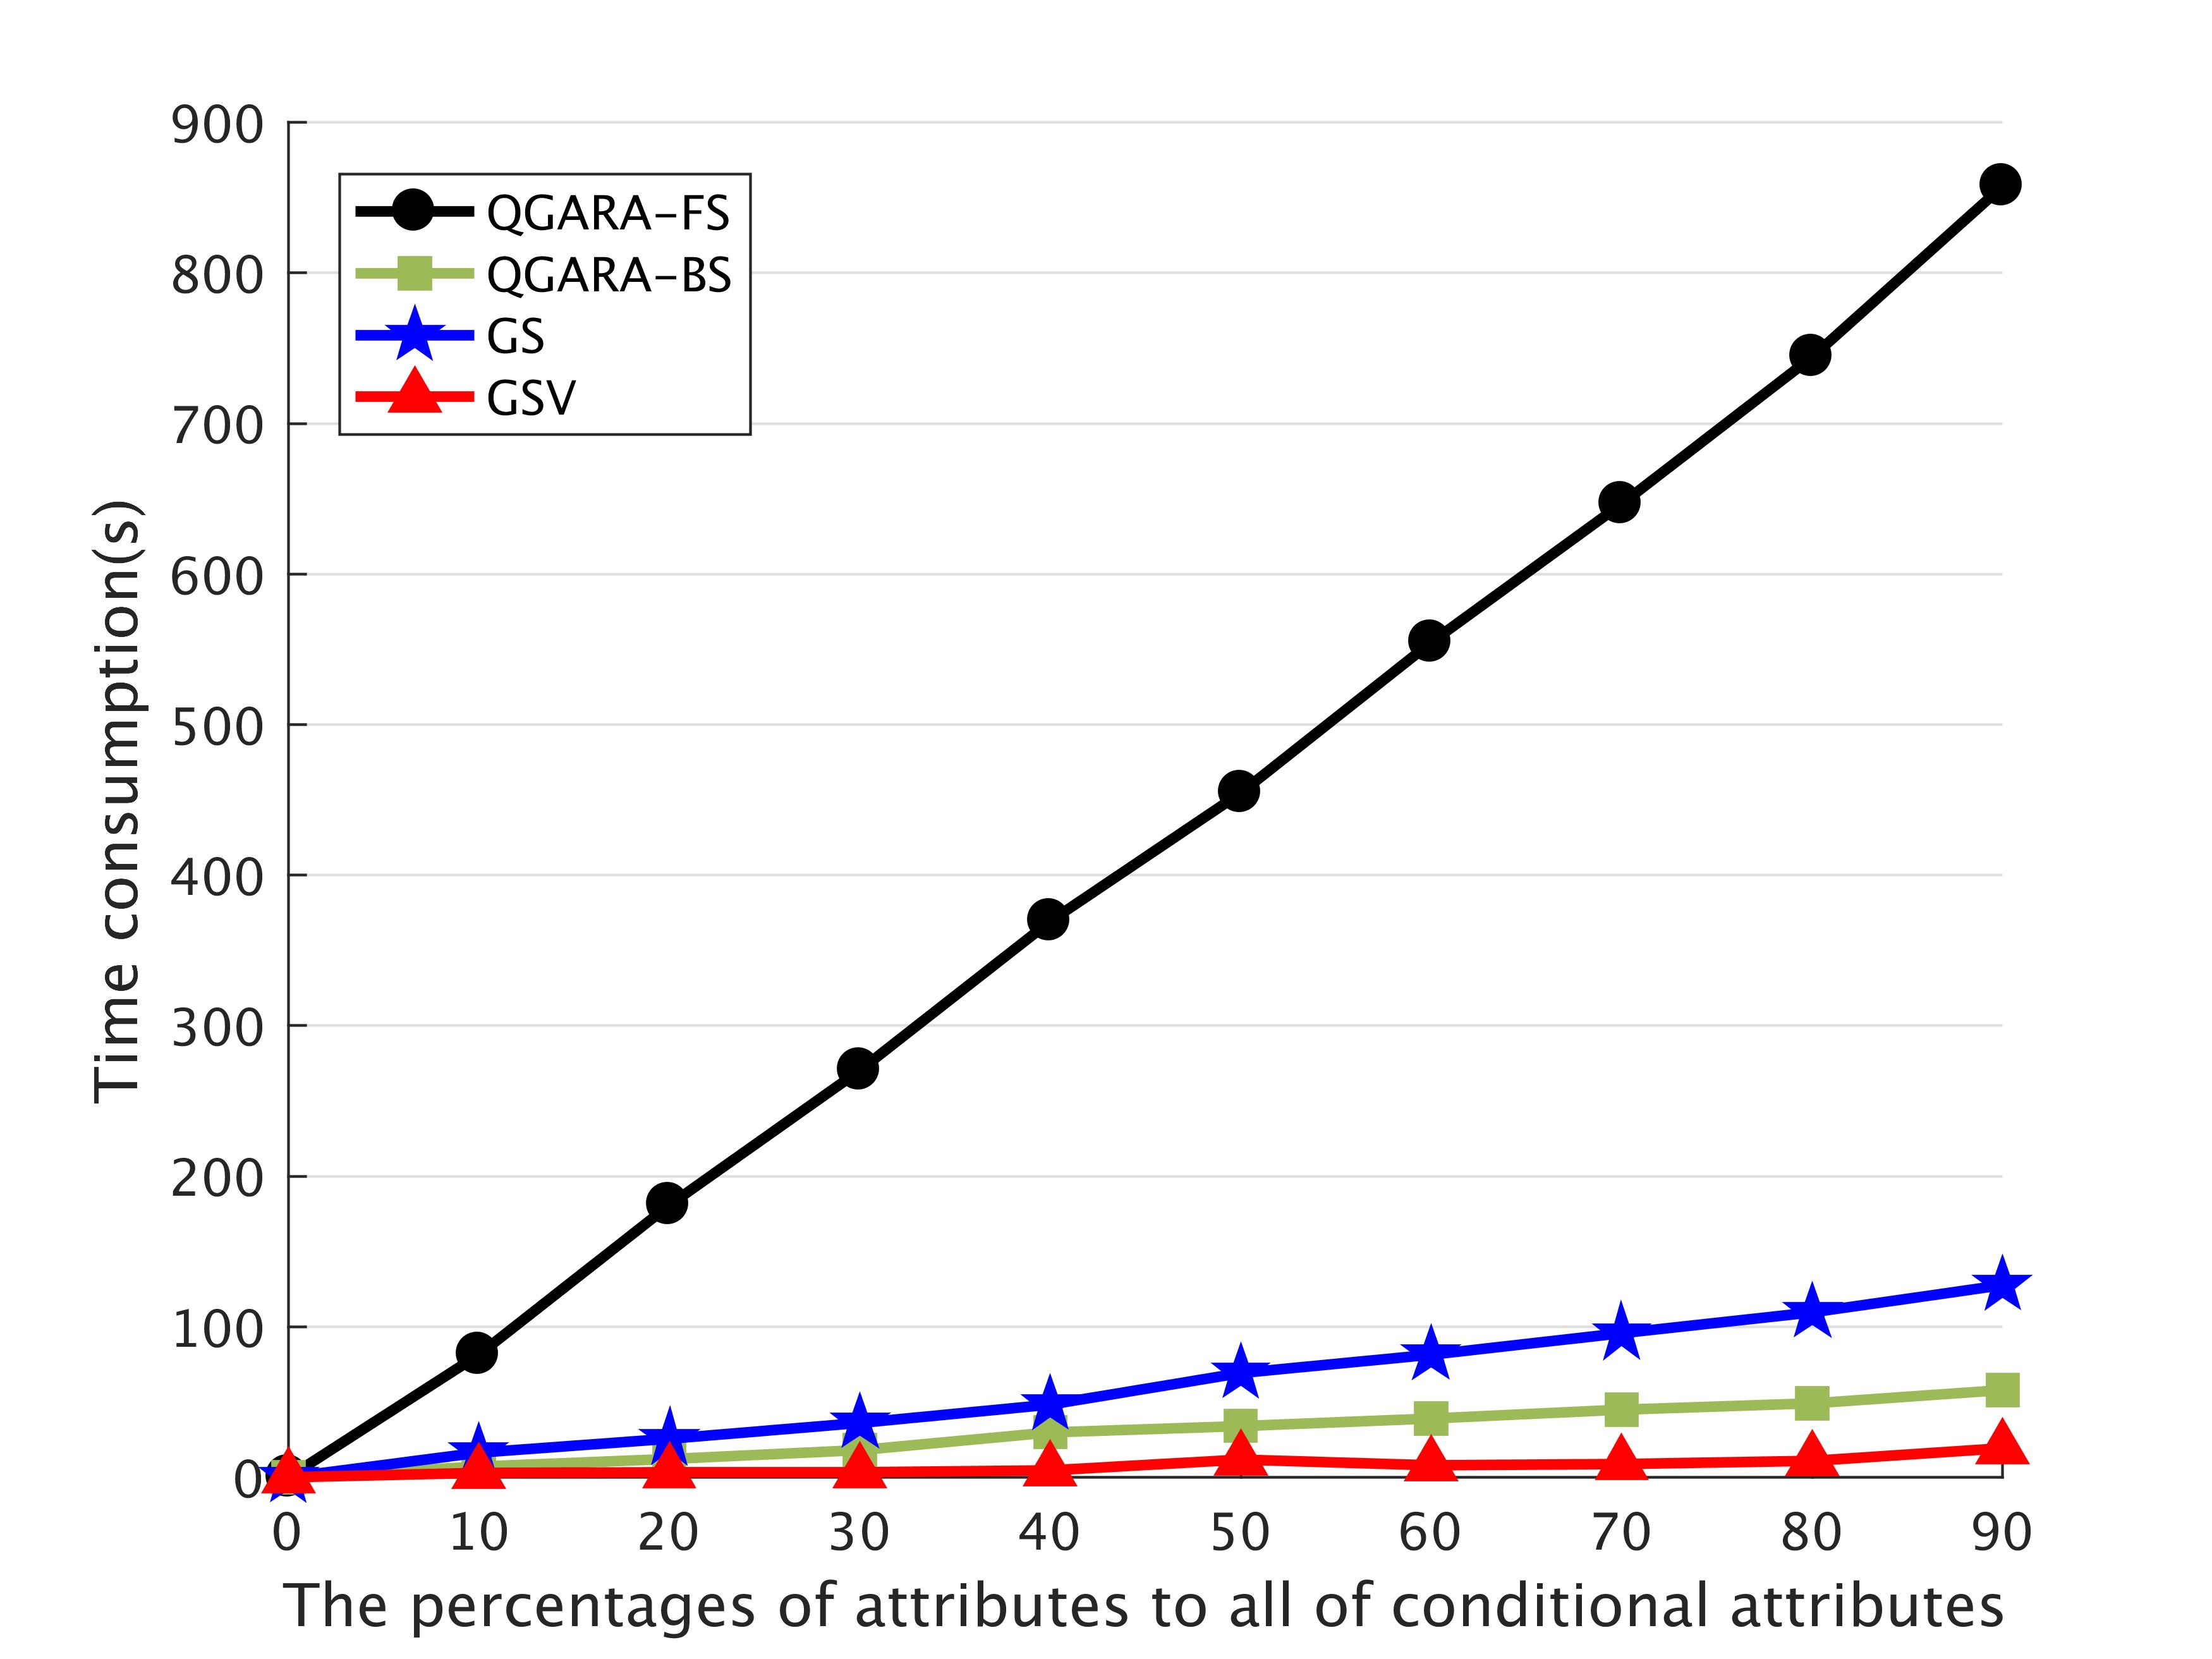
\includegraphics[width=5cm]{./Curve_universe/10_cnnect4_pos.jpg} 
			}
			\caption{Time of general reduction algorithms versus the size of objects} 
			\label{TimeIncreaseObjects}
		\end{figure}
		
		\begin{figure}[htbp]
			\centering 
			\subfigure[Mushroom]{
				\label{Fig.sub2.2}
				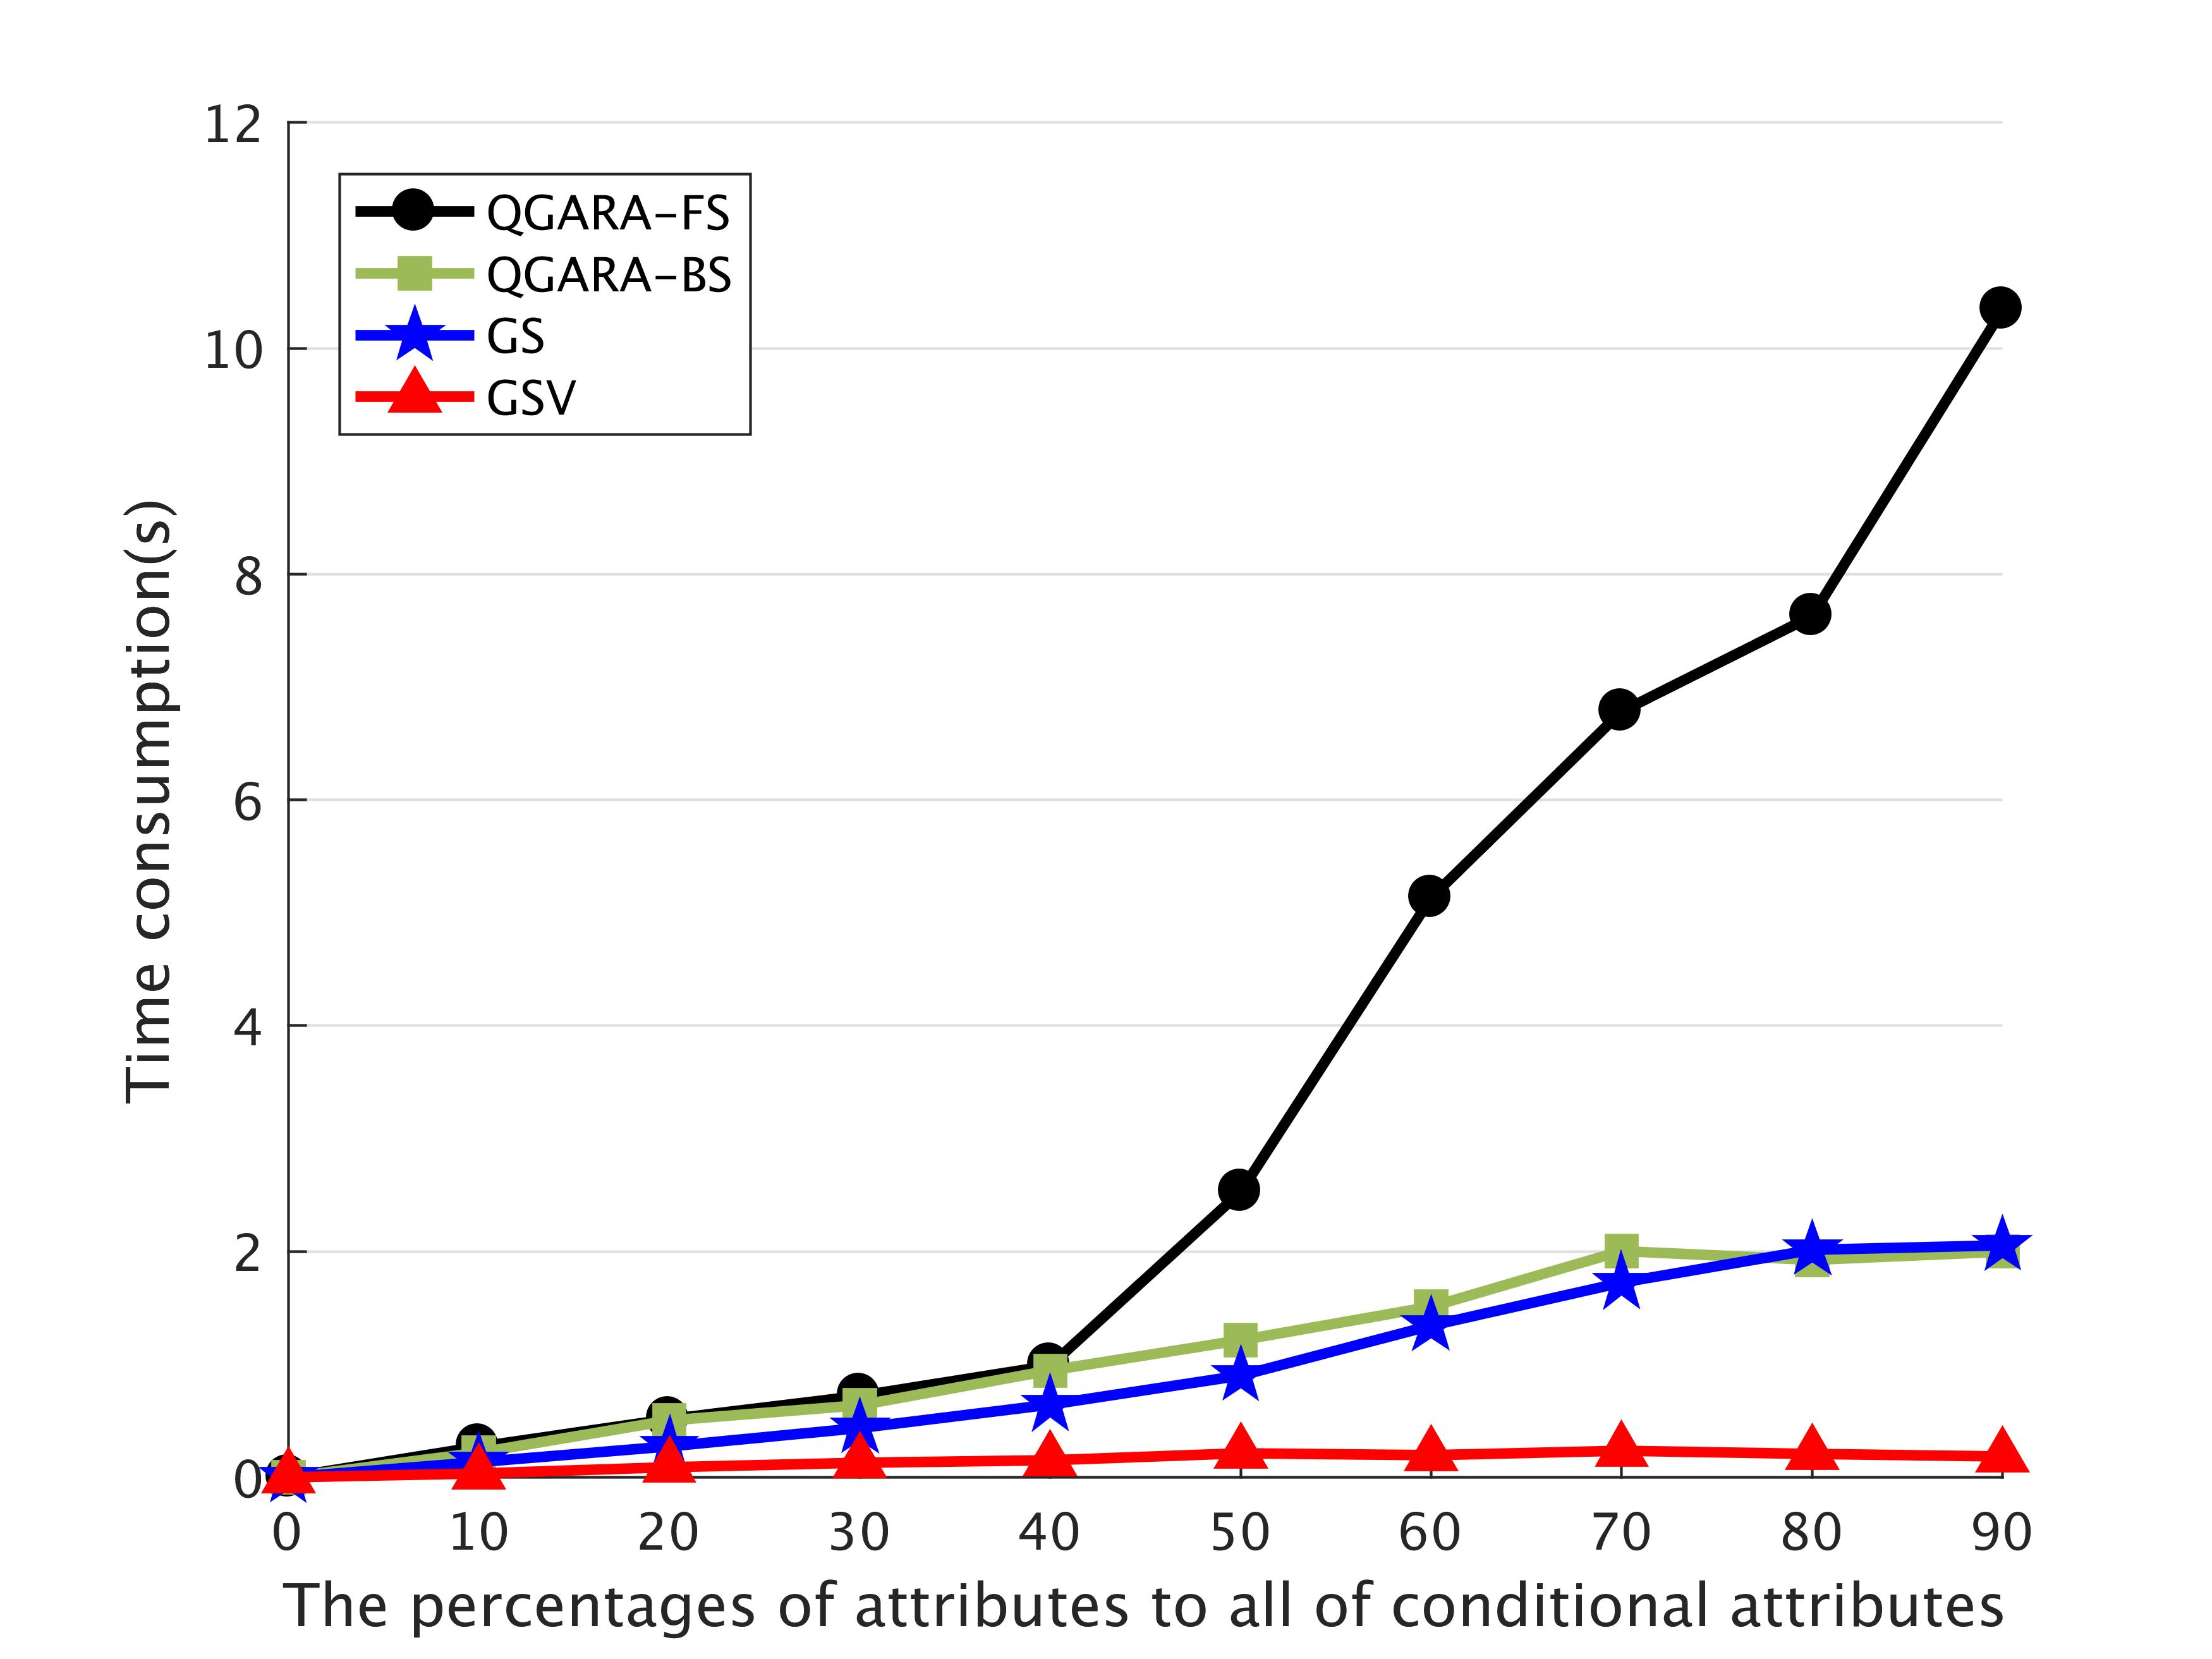
\includegraphics[width=5cm]{./Curve_attributes/1_mushroom_pos.jpg} 
			}
			\subfigure[Tic]{
				\label{Fig.sub2.3}
				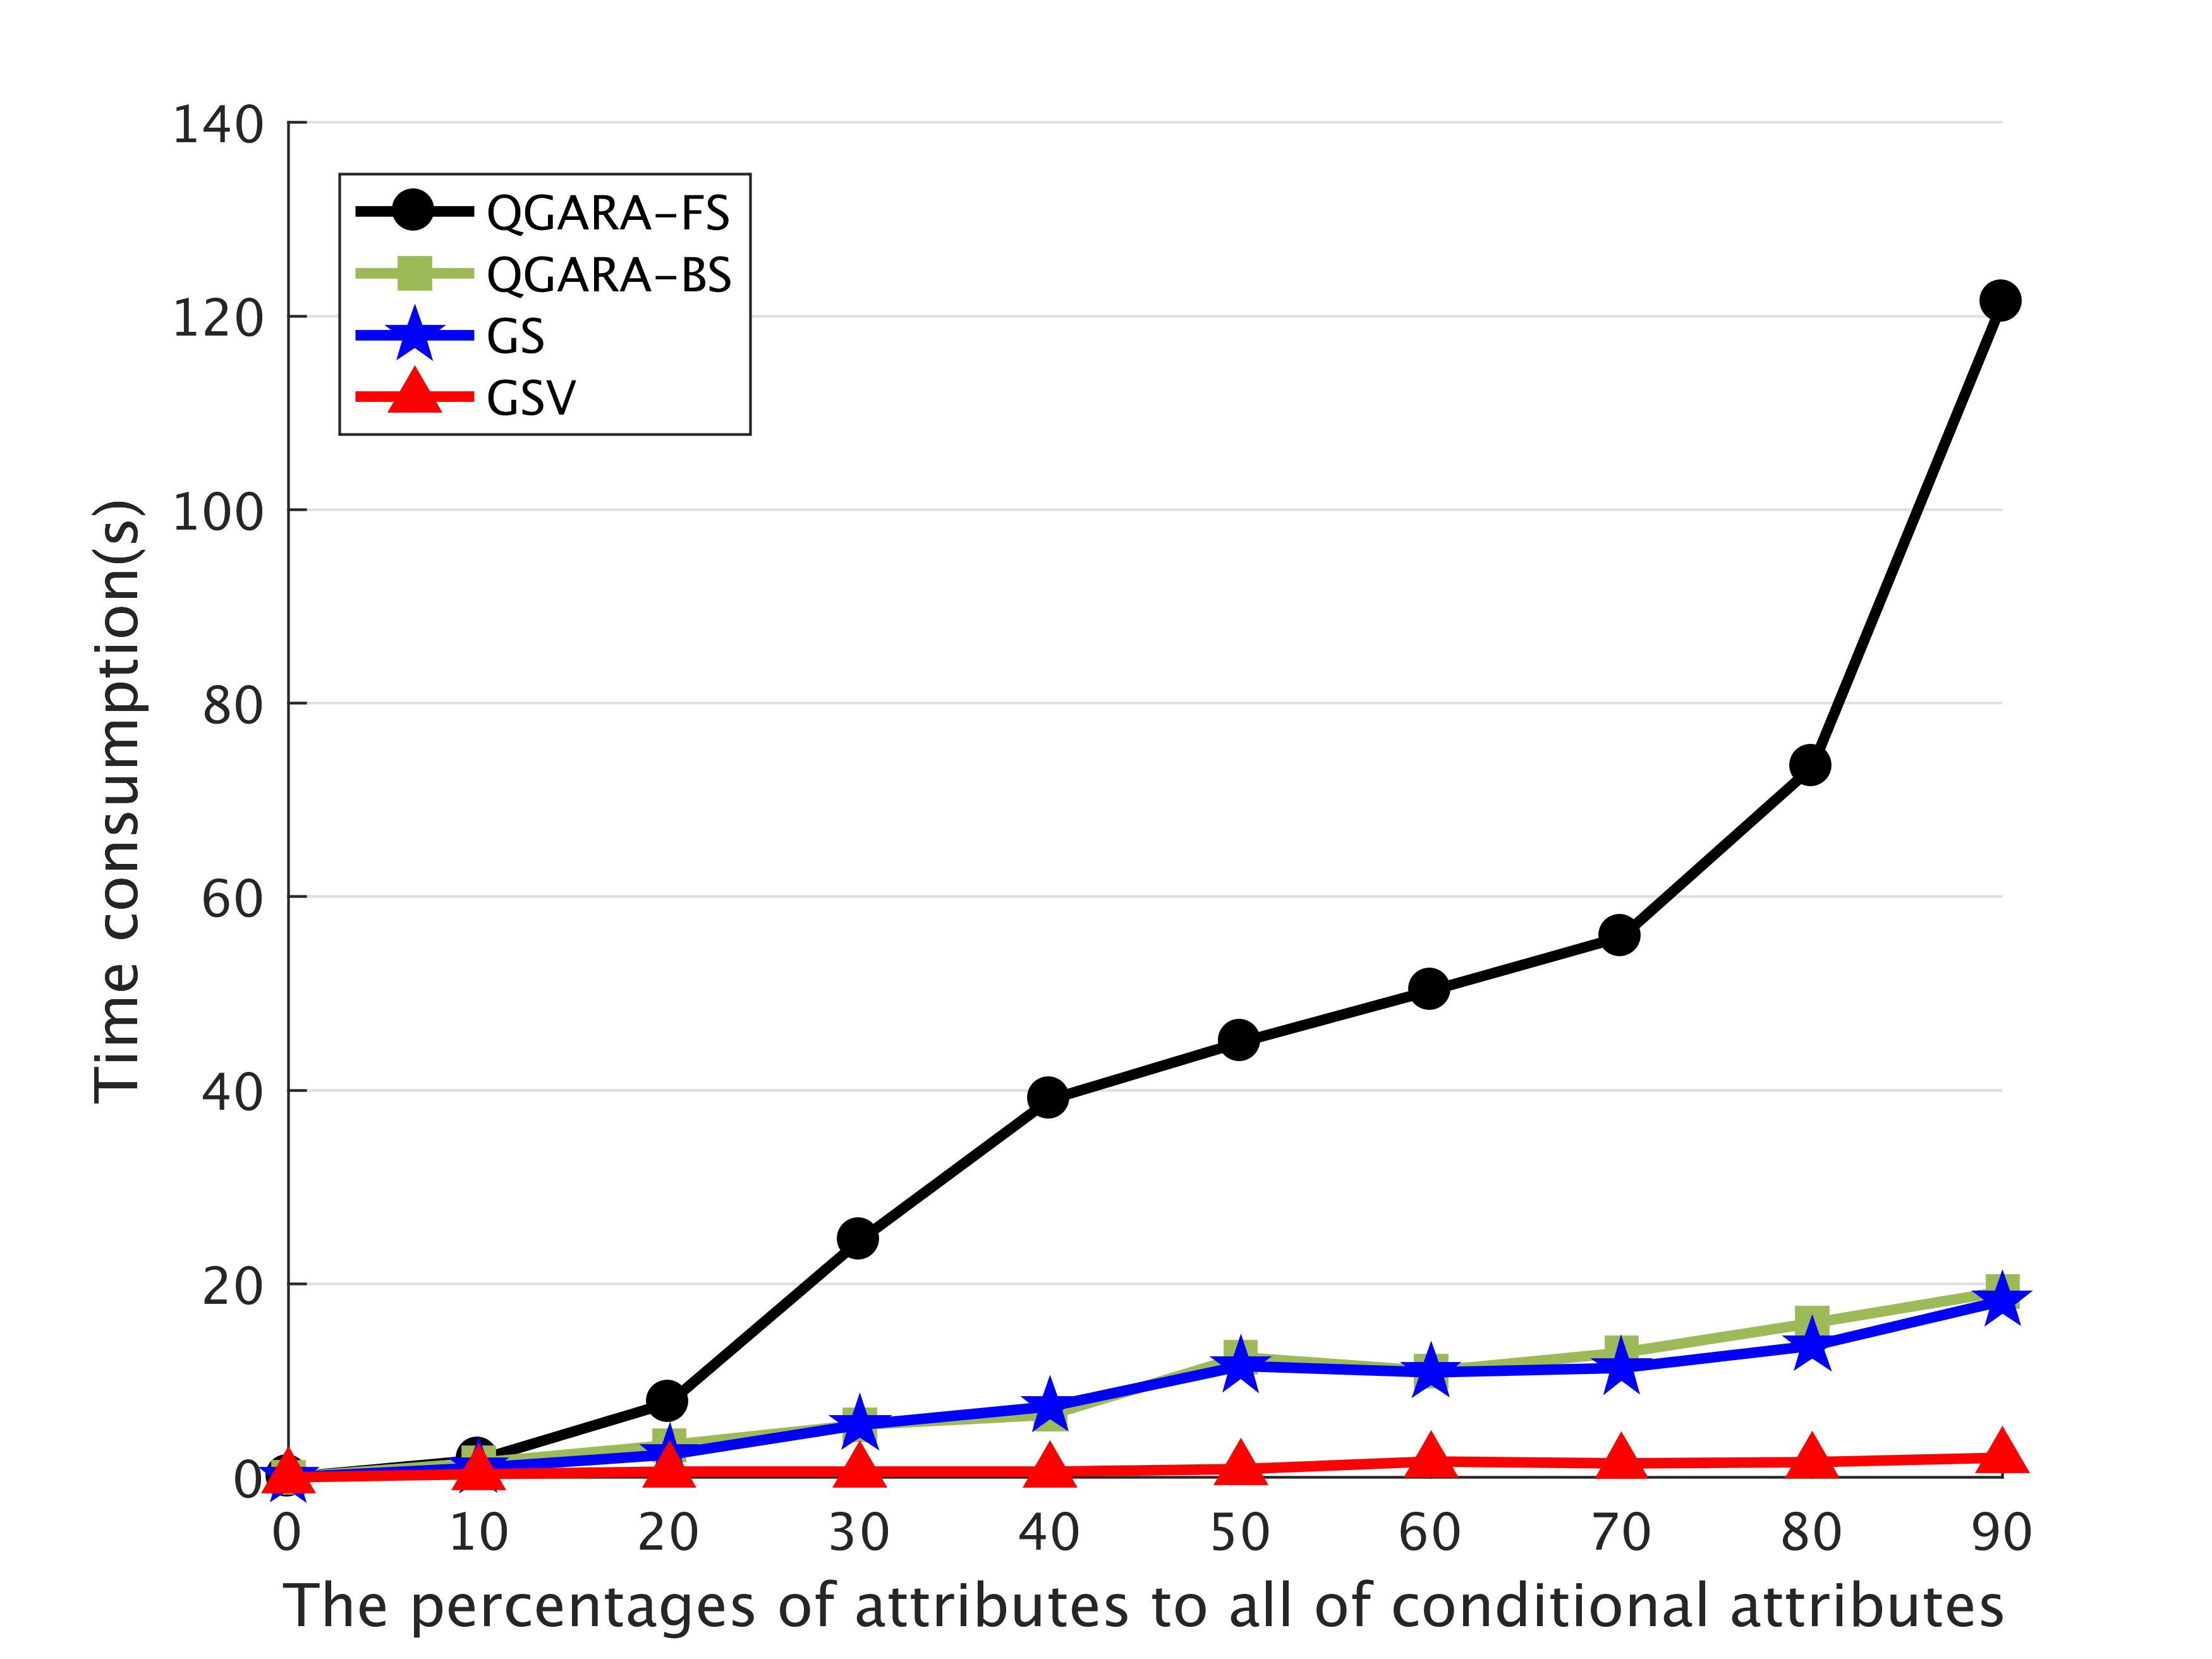
\includegraphics[width=5cm]{./Curve_attributes/2_tic_pos.jpg} 
			}
			\subfigure[Segmentation]{
				\label{Fig.sub2.4}
				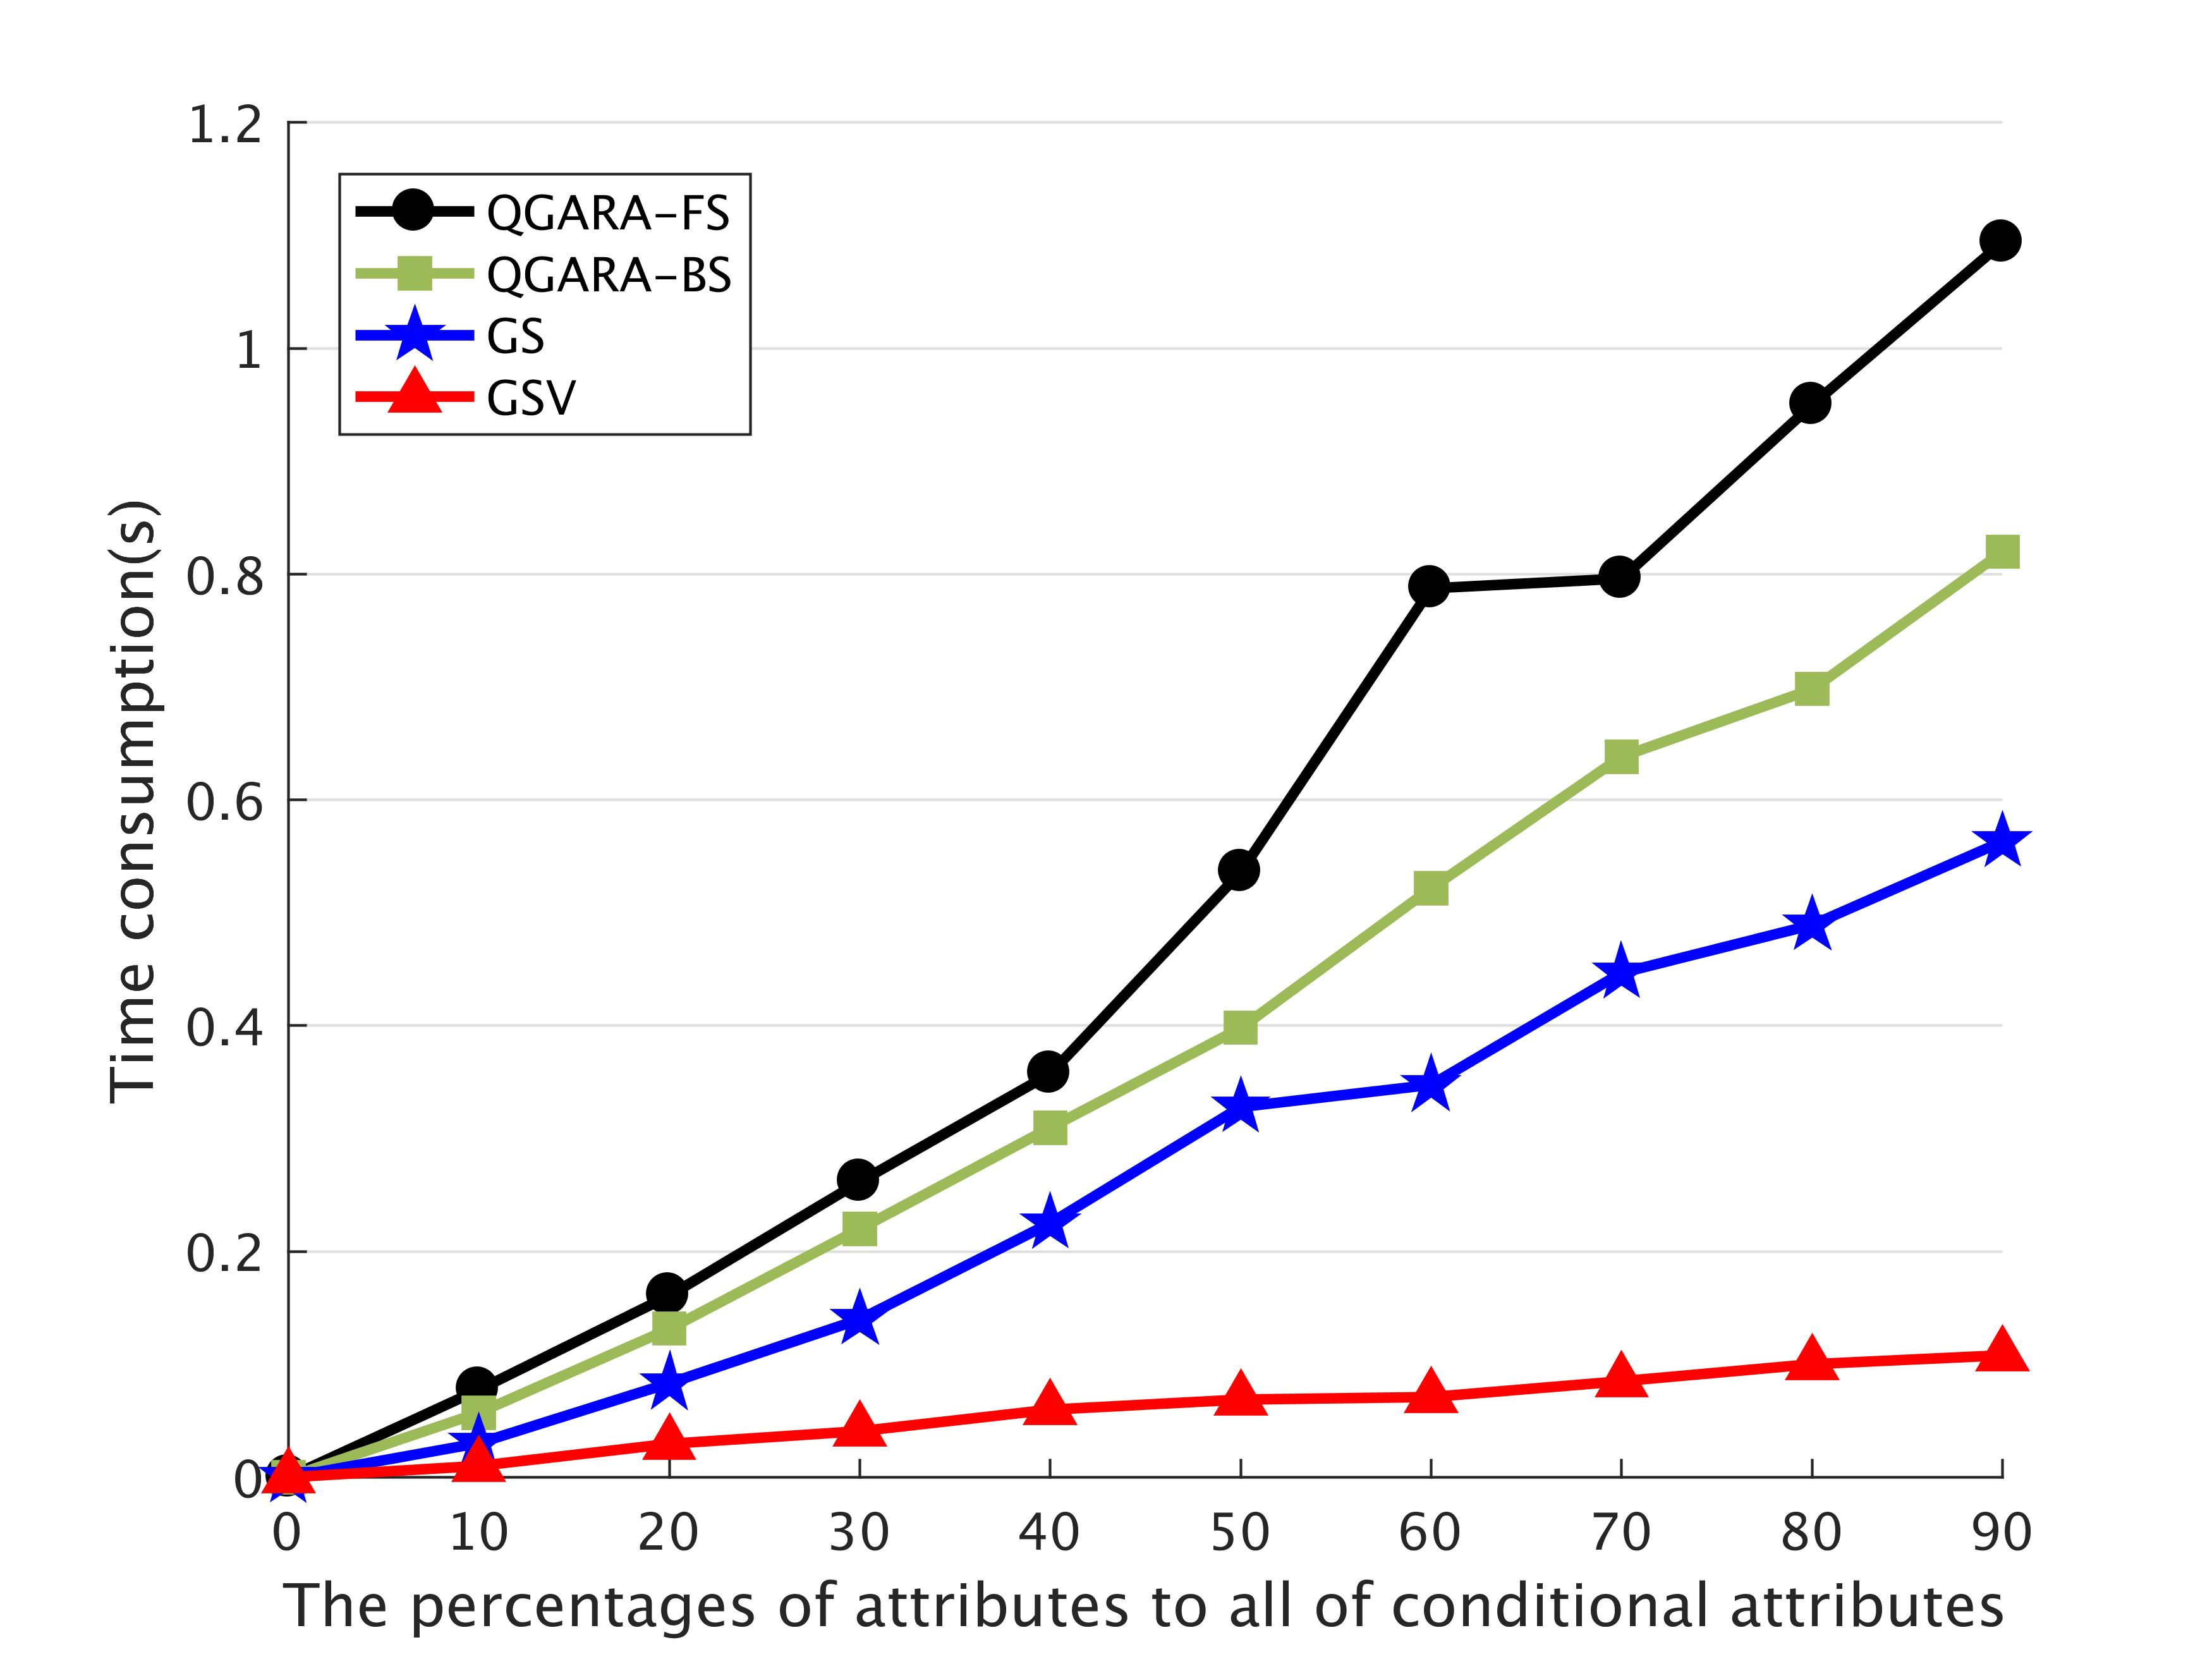
\includegraphics[width=5cm]{./Curve_attributes/3_seg_pos.jpg} 
			}
			\subfigure[Splice]{
				\label{Fig.sub2.6}
				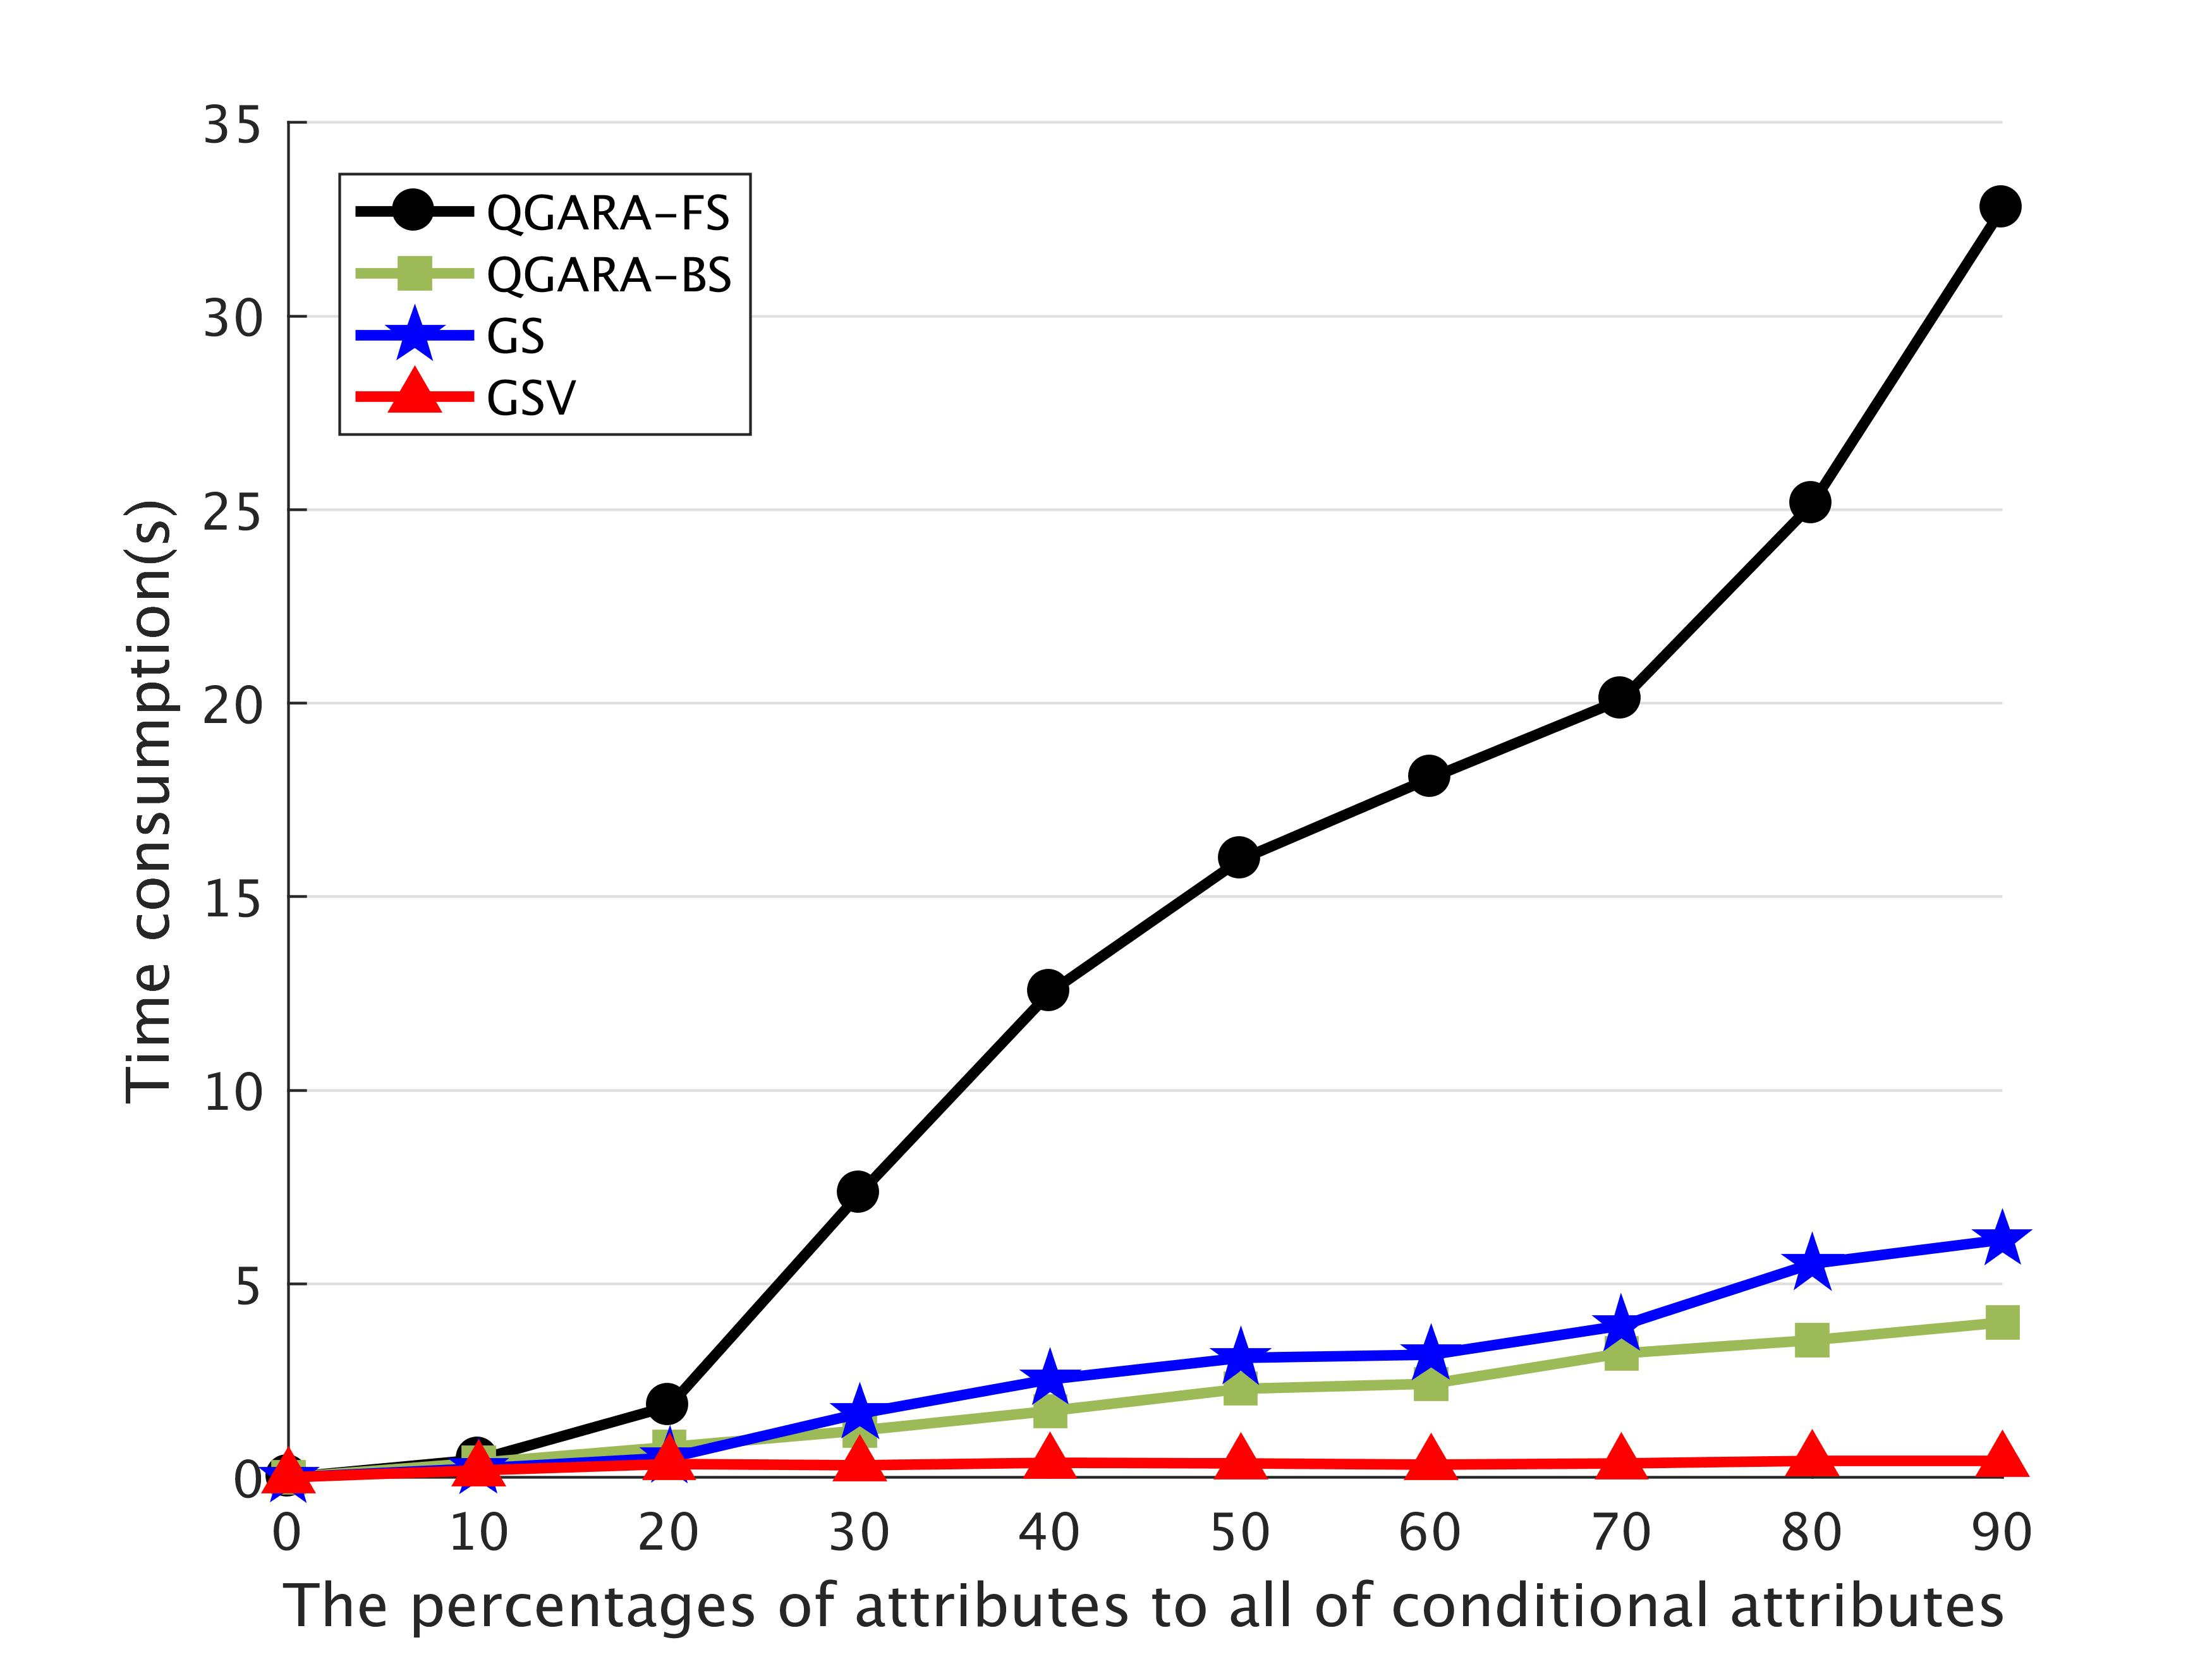
\includegraphics[width=5cm]{./Curve_attributes/4_splice_pos.jpg} 
			}
			\subfigure[Dermatology]{
				\label{Fig.sub2.7}
				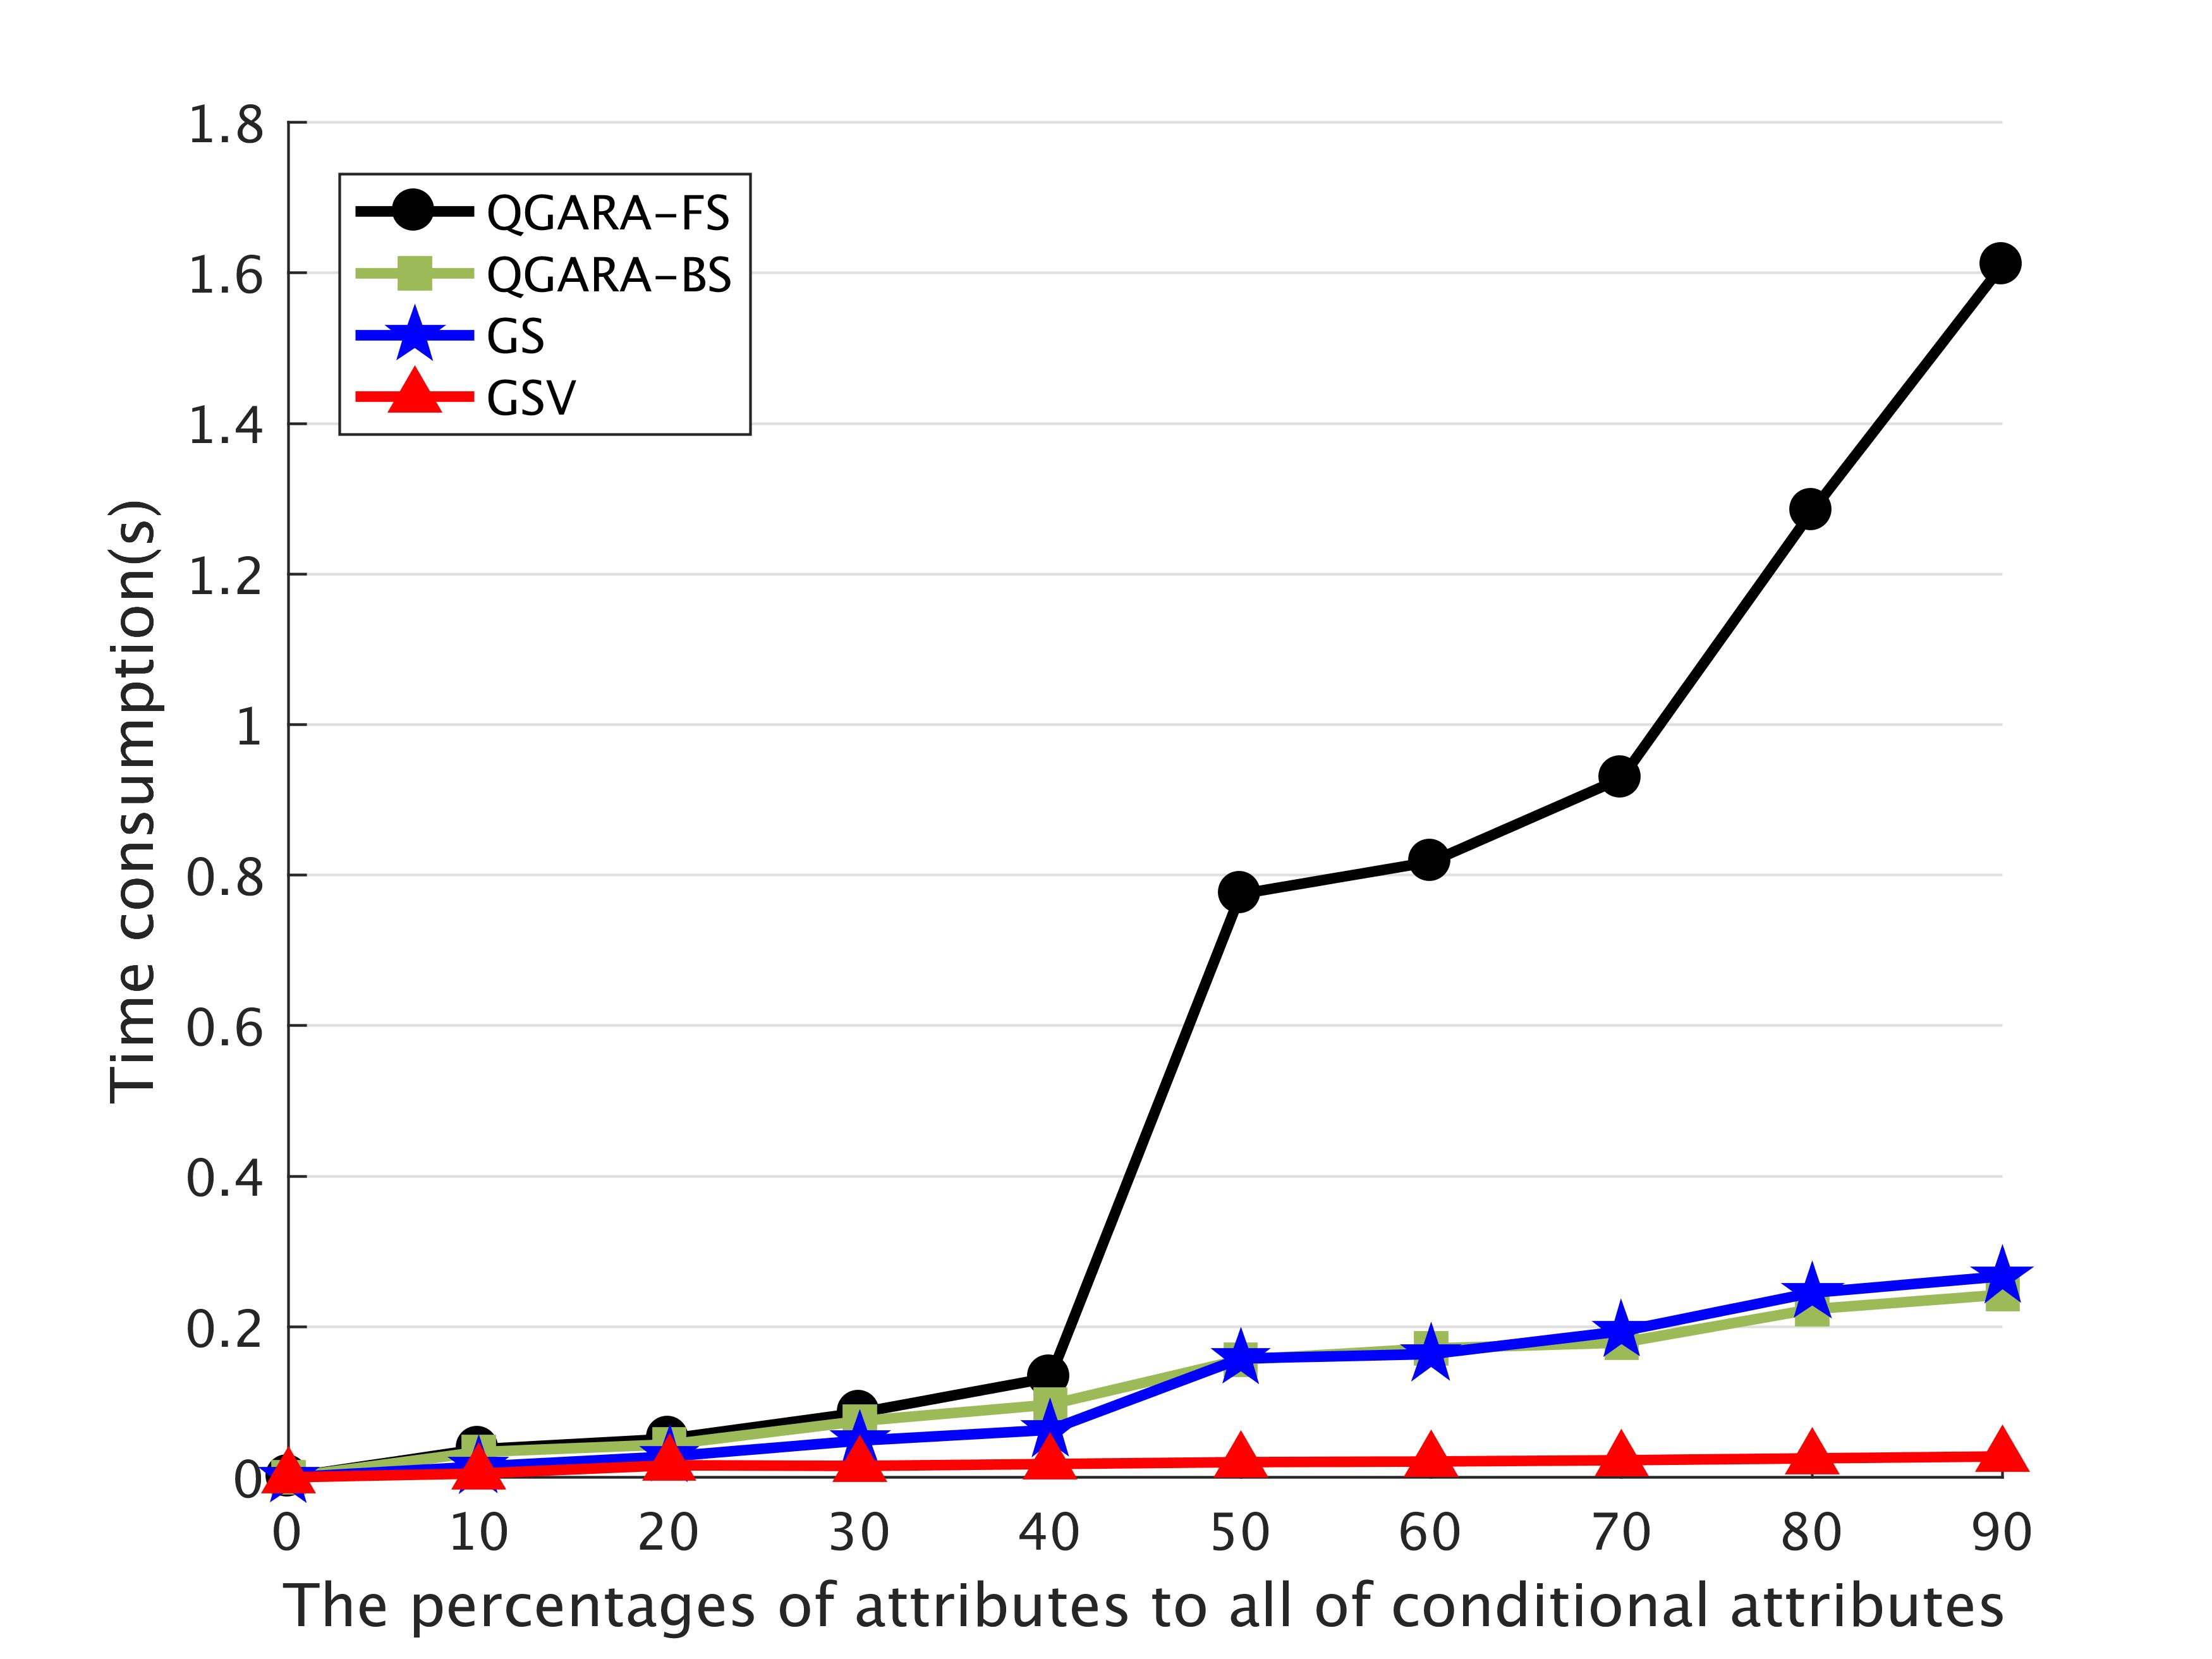
\includegraphics[width=5cm]{./Curve_attributes/5_dermatology_pos.jpg} 
			}
			\subfigure[Wdbc]{
				\label{Fig.sub2.8}
				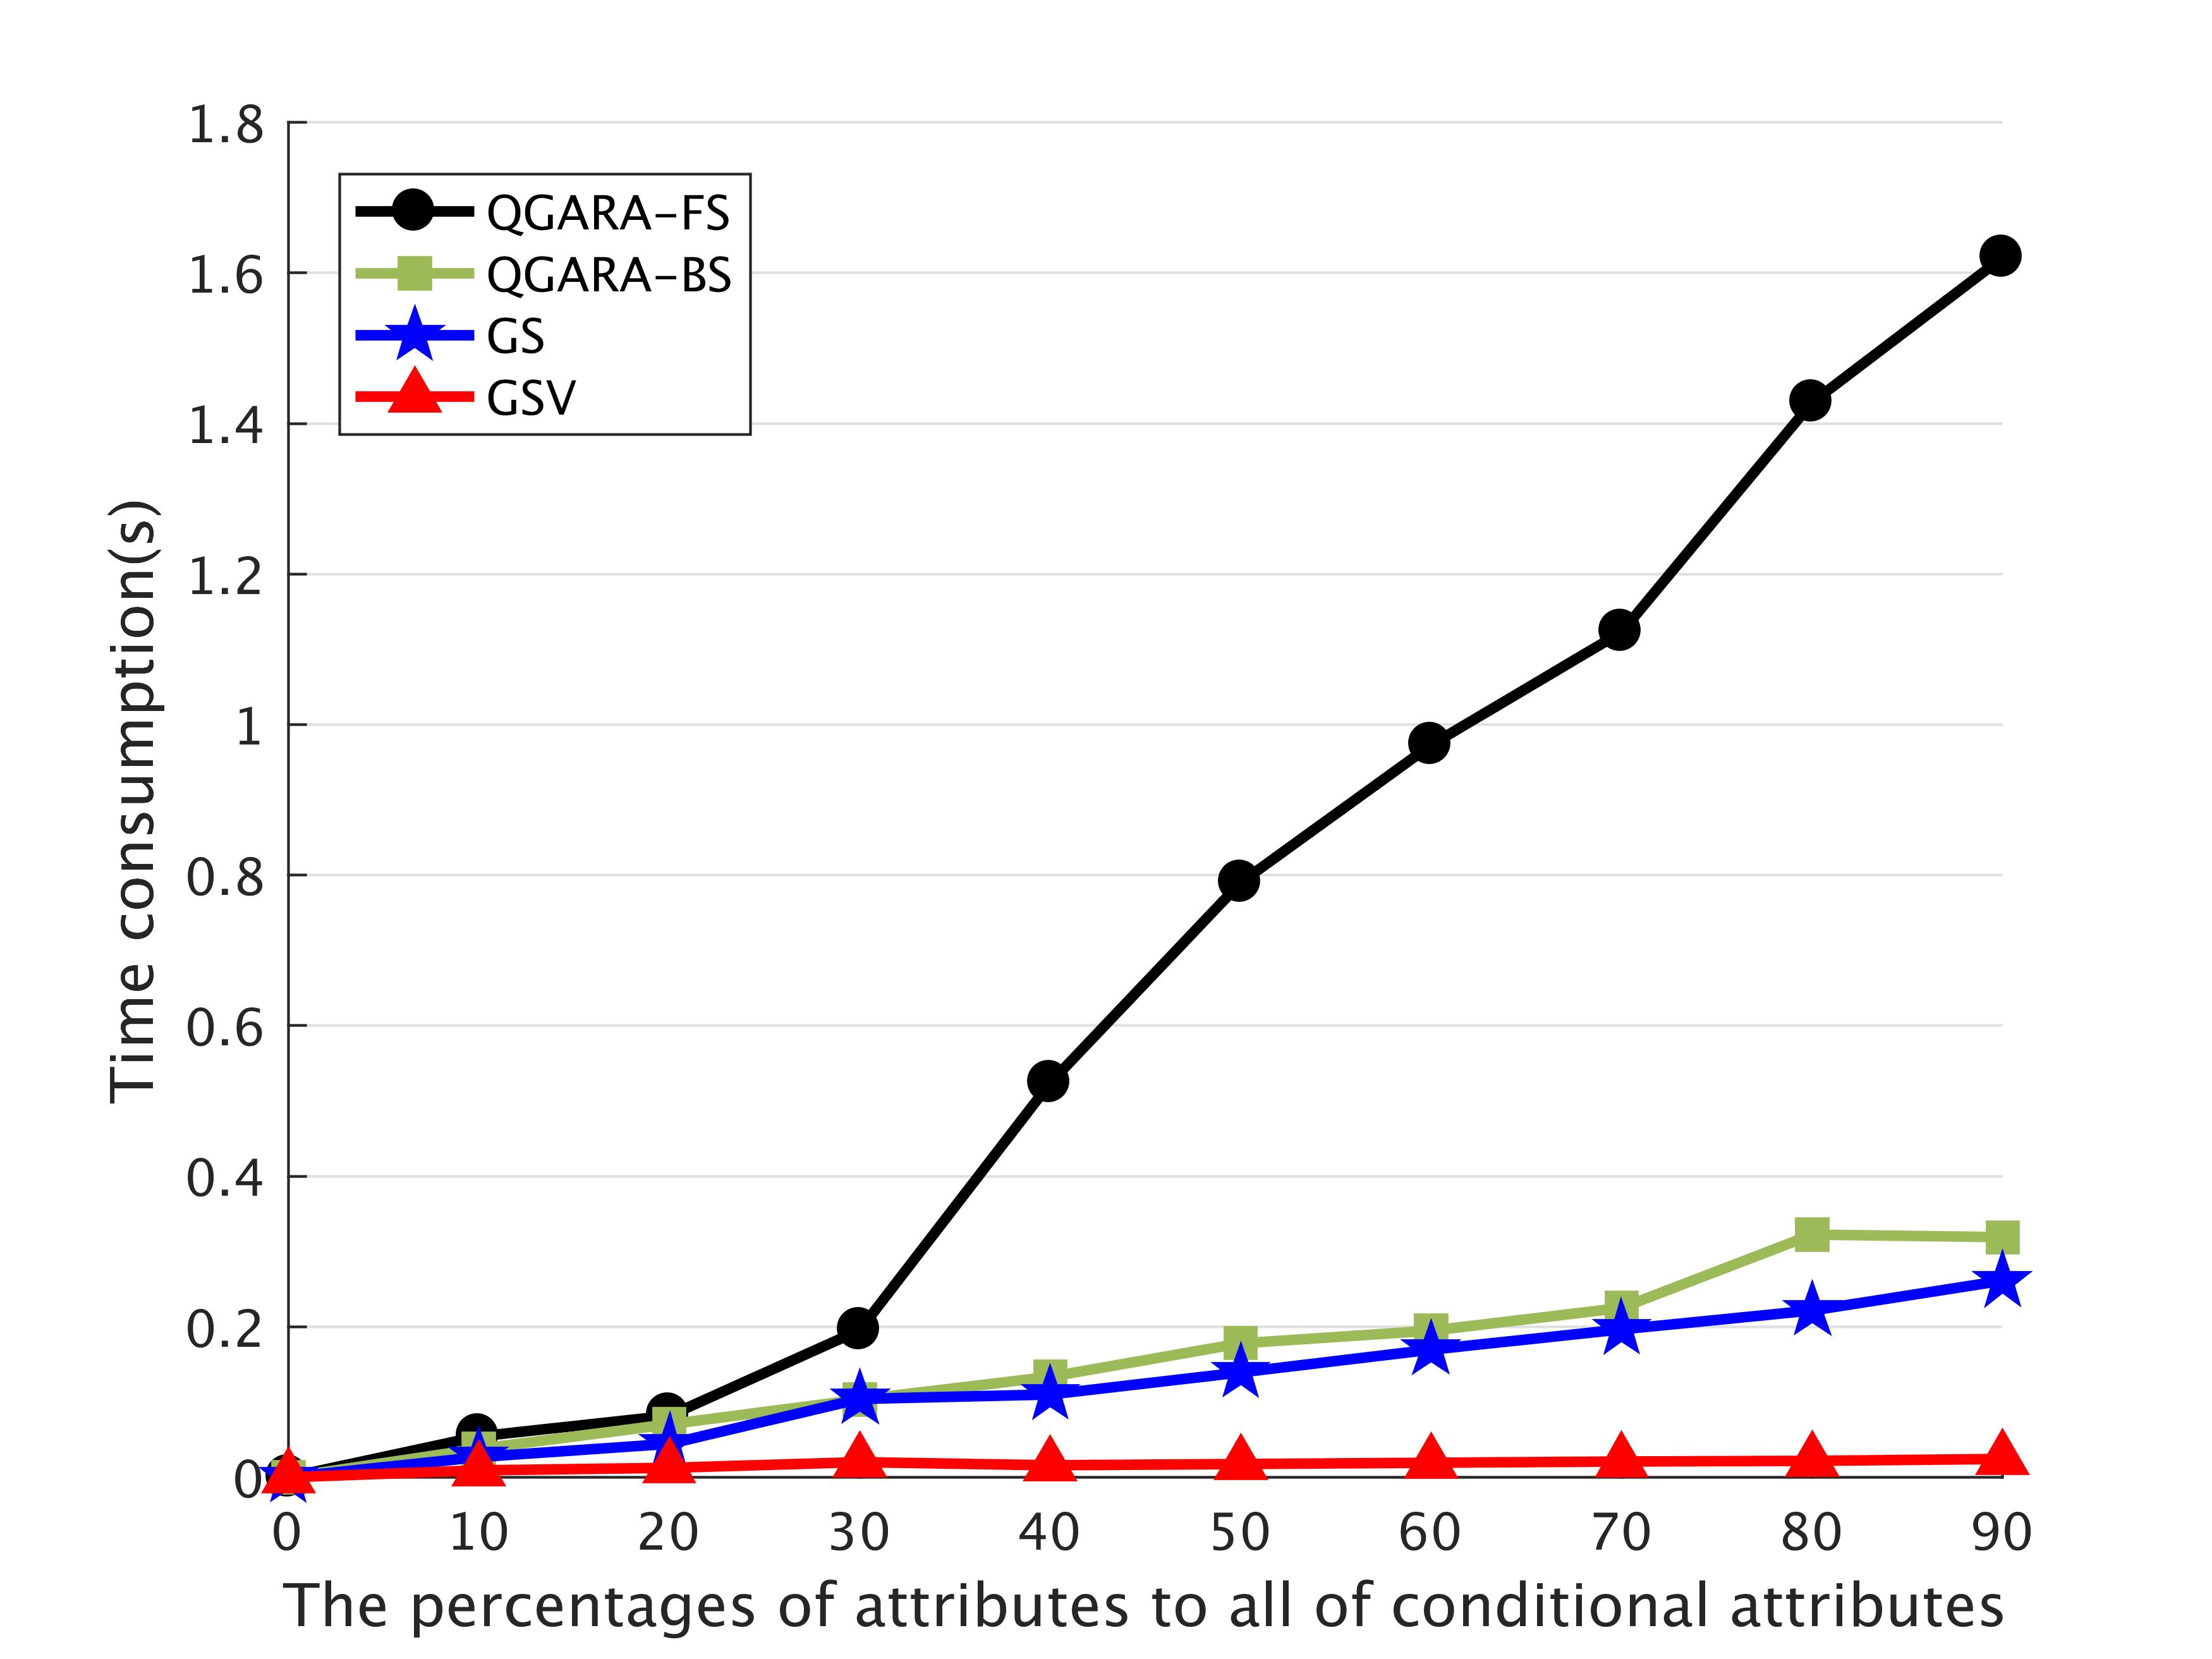
\includegraphics[width=5cm]{./Curve_attributes/6_wdbc_pos.jpg} 
			}
			%		\end{figure}
			%		\begin{figure}[htbp]
			\subfigure[CNAE9]{
				\label{Fig.sub2.9}
				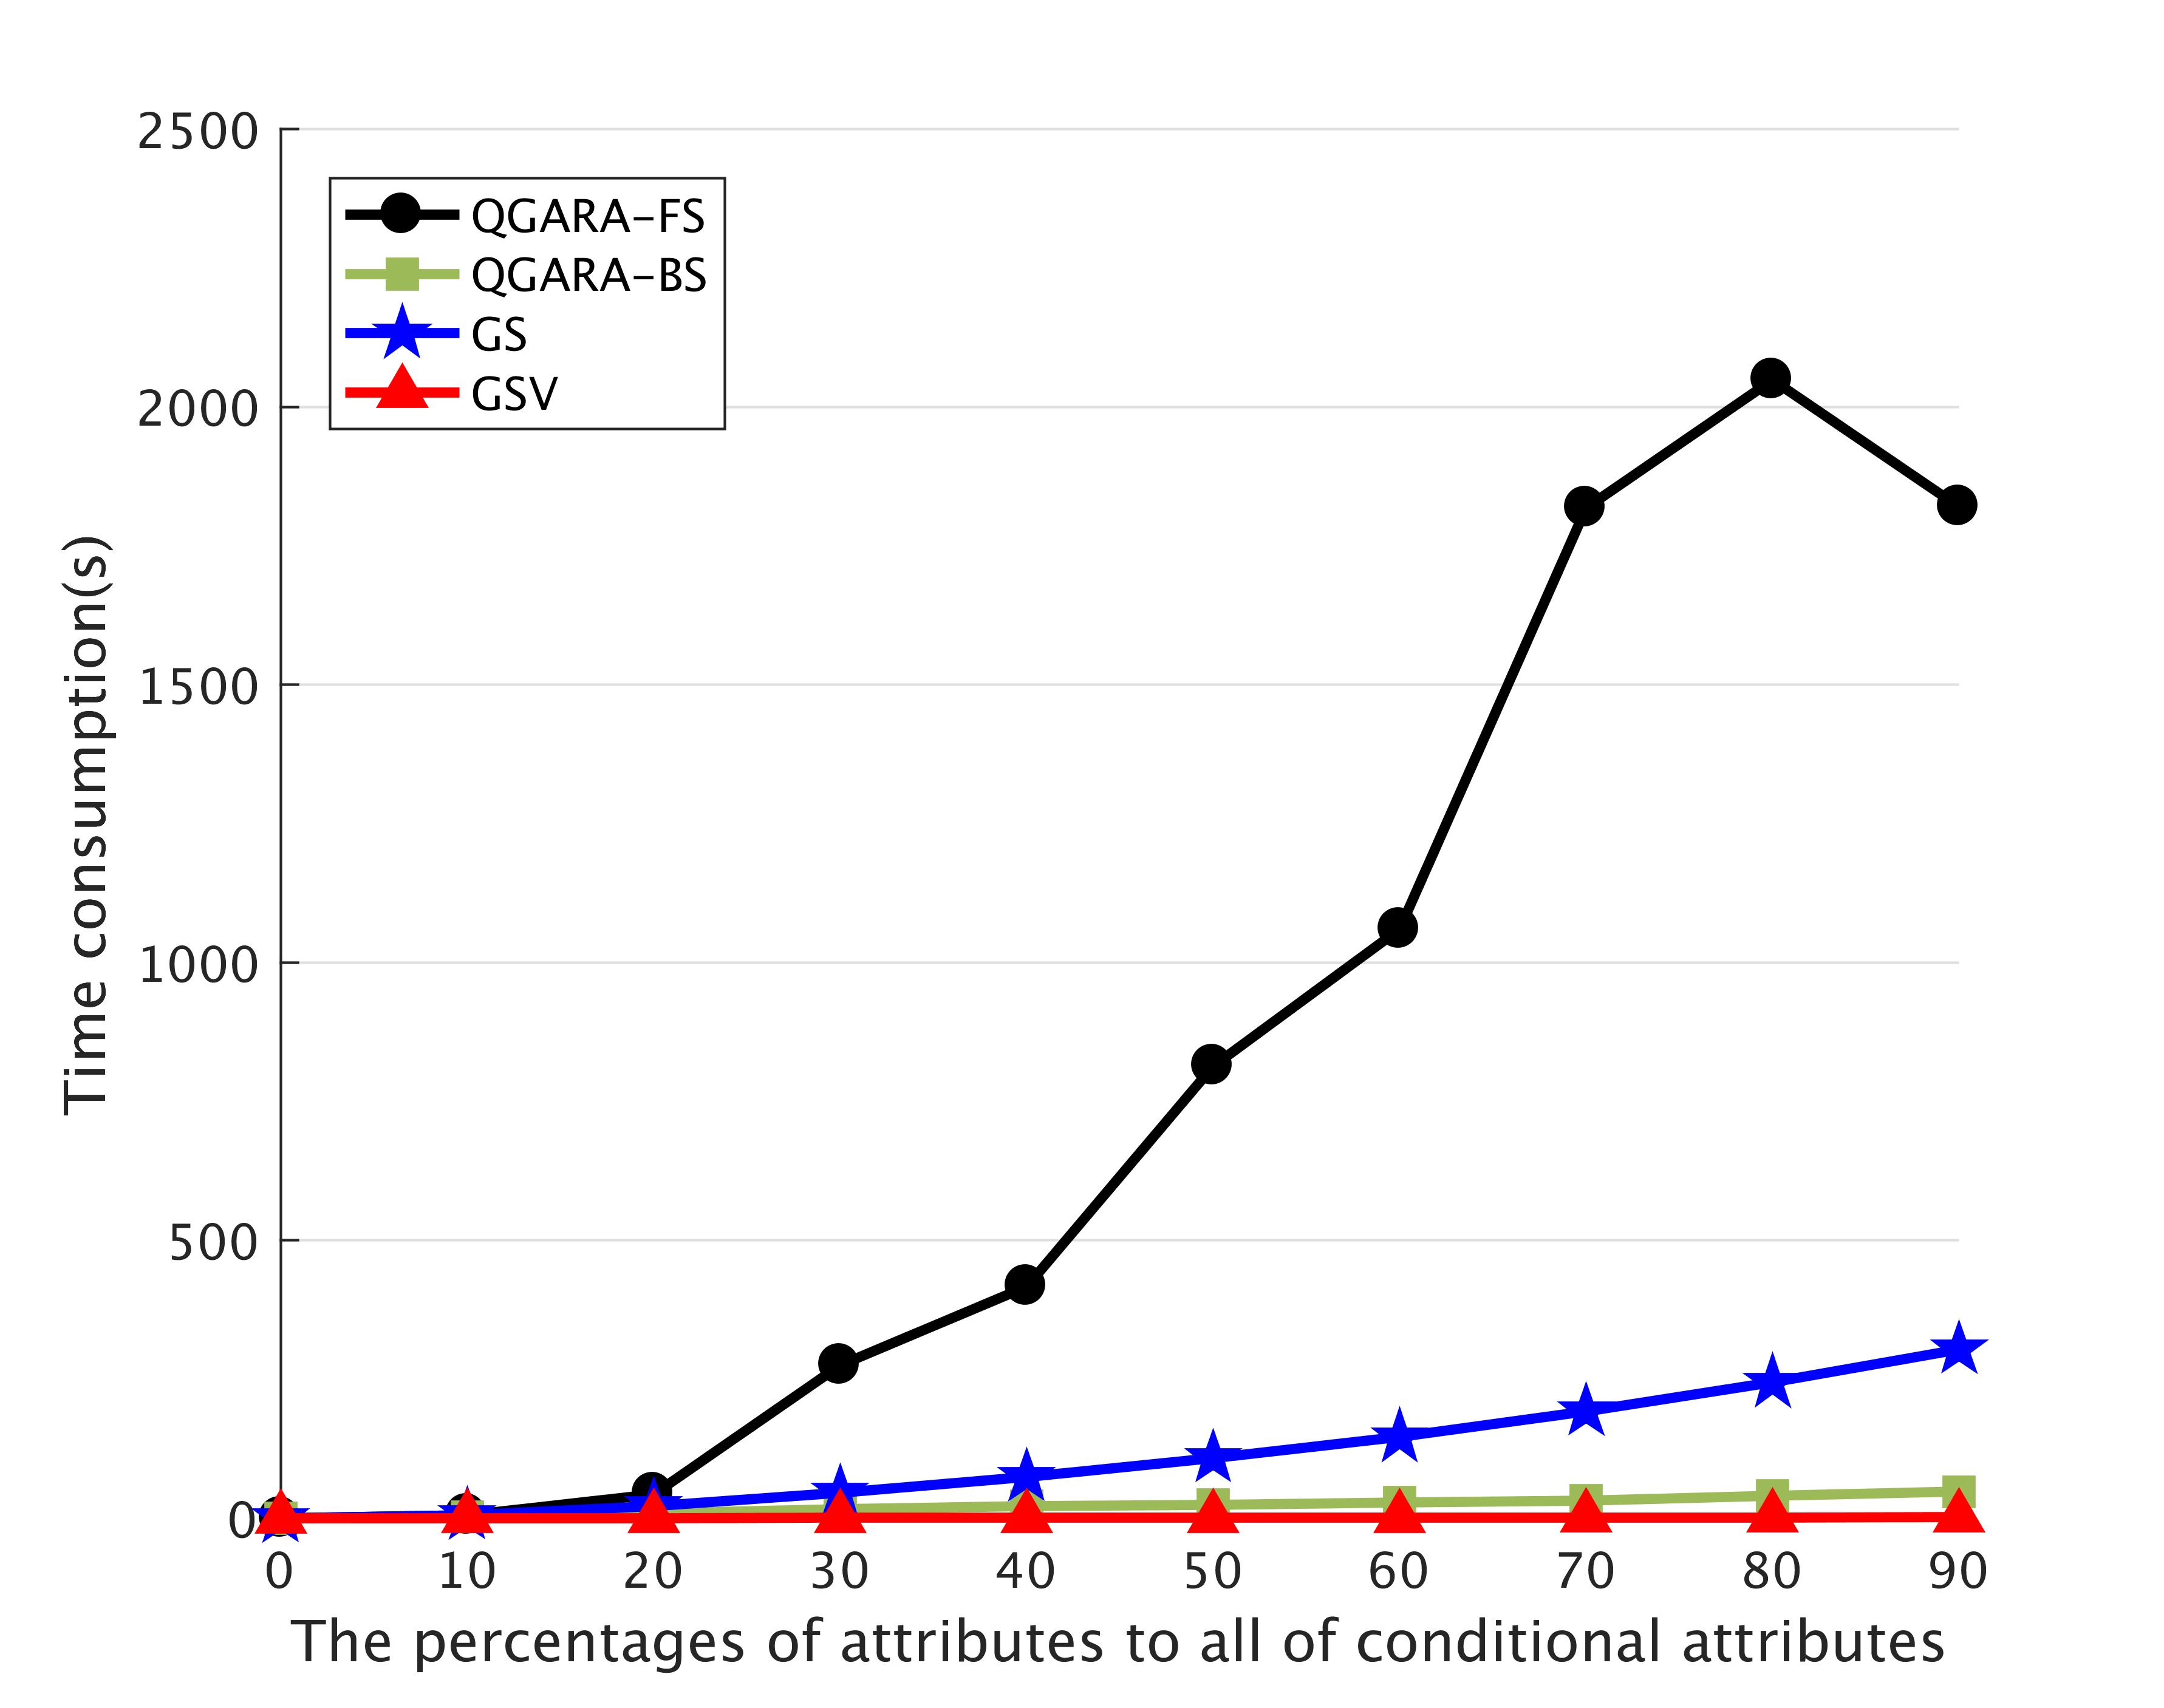
\includegraphics[width=5cm]{./Curve_attributes/9.jpg} 
			}
%			\subfigure[Semeion]{
%				\label{Fig.sub2.10}
%				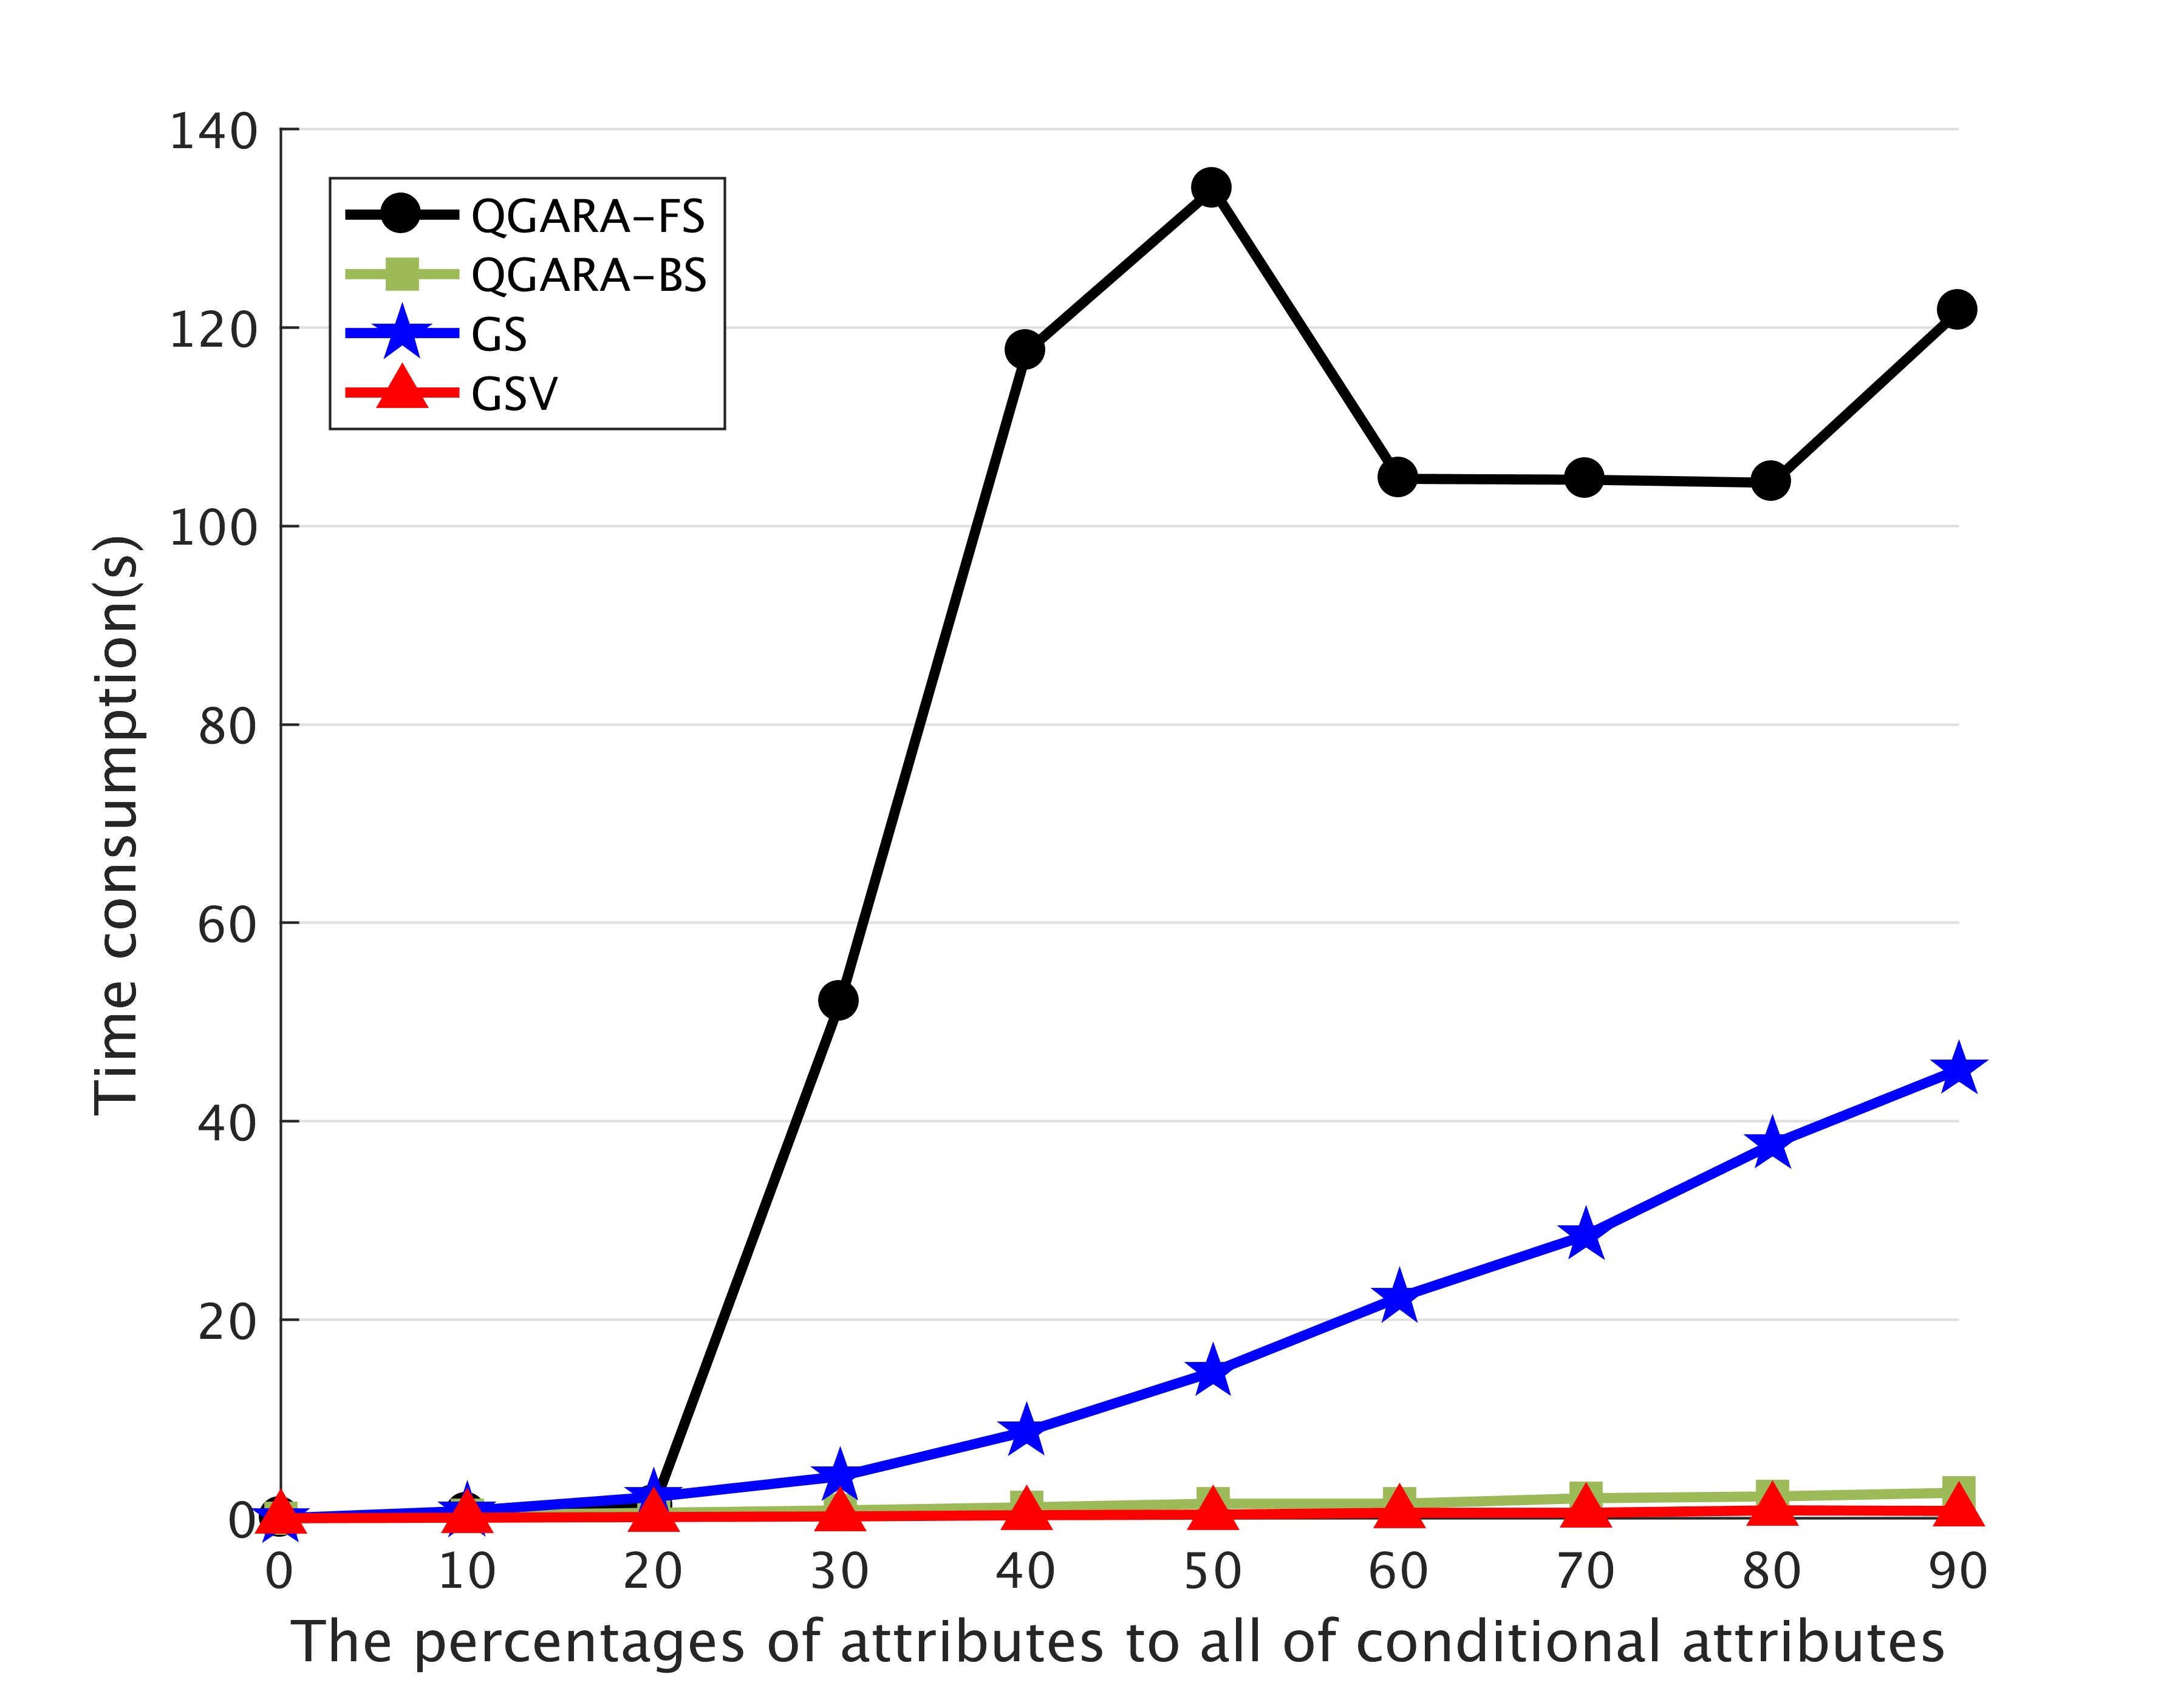
\includegraphics[width=5cm]{./Curve_attributes/10.jpg} 
%			}
			\subfigure[DNA]{
				\label{Fig.sub2.11}
				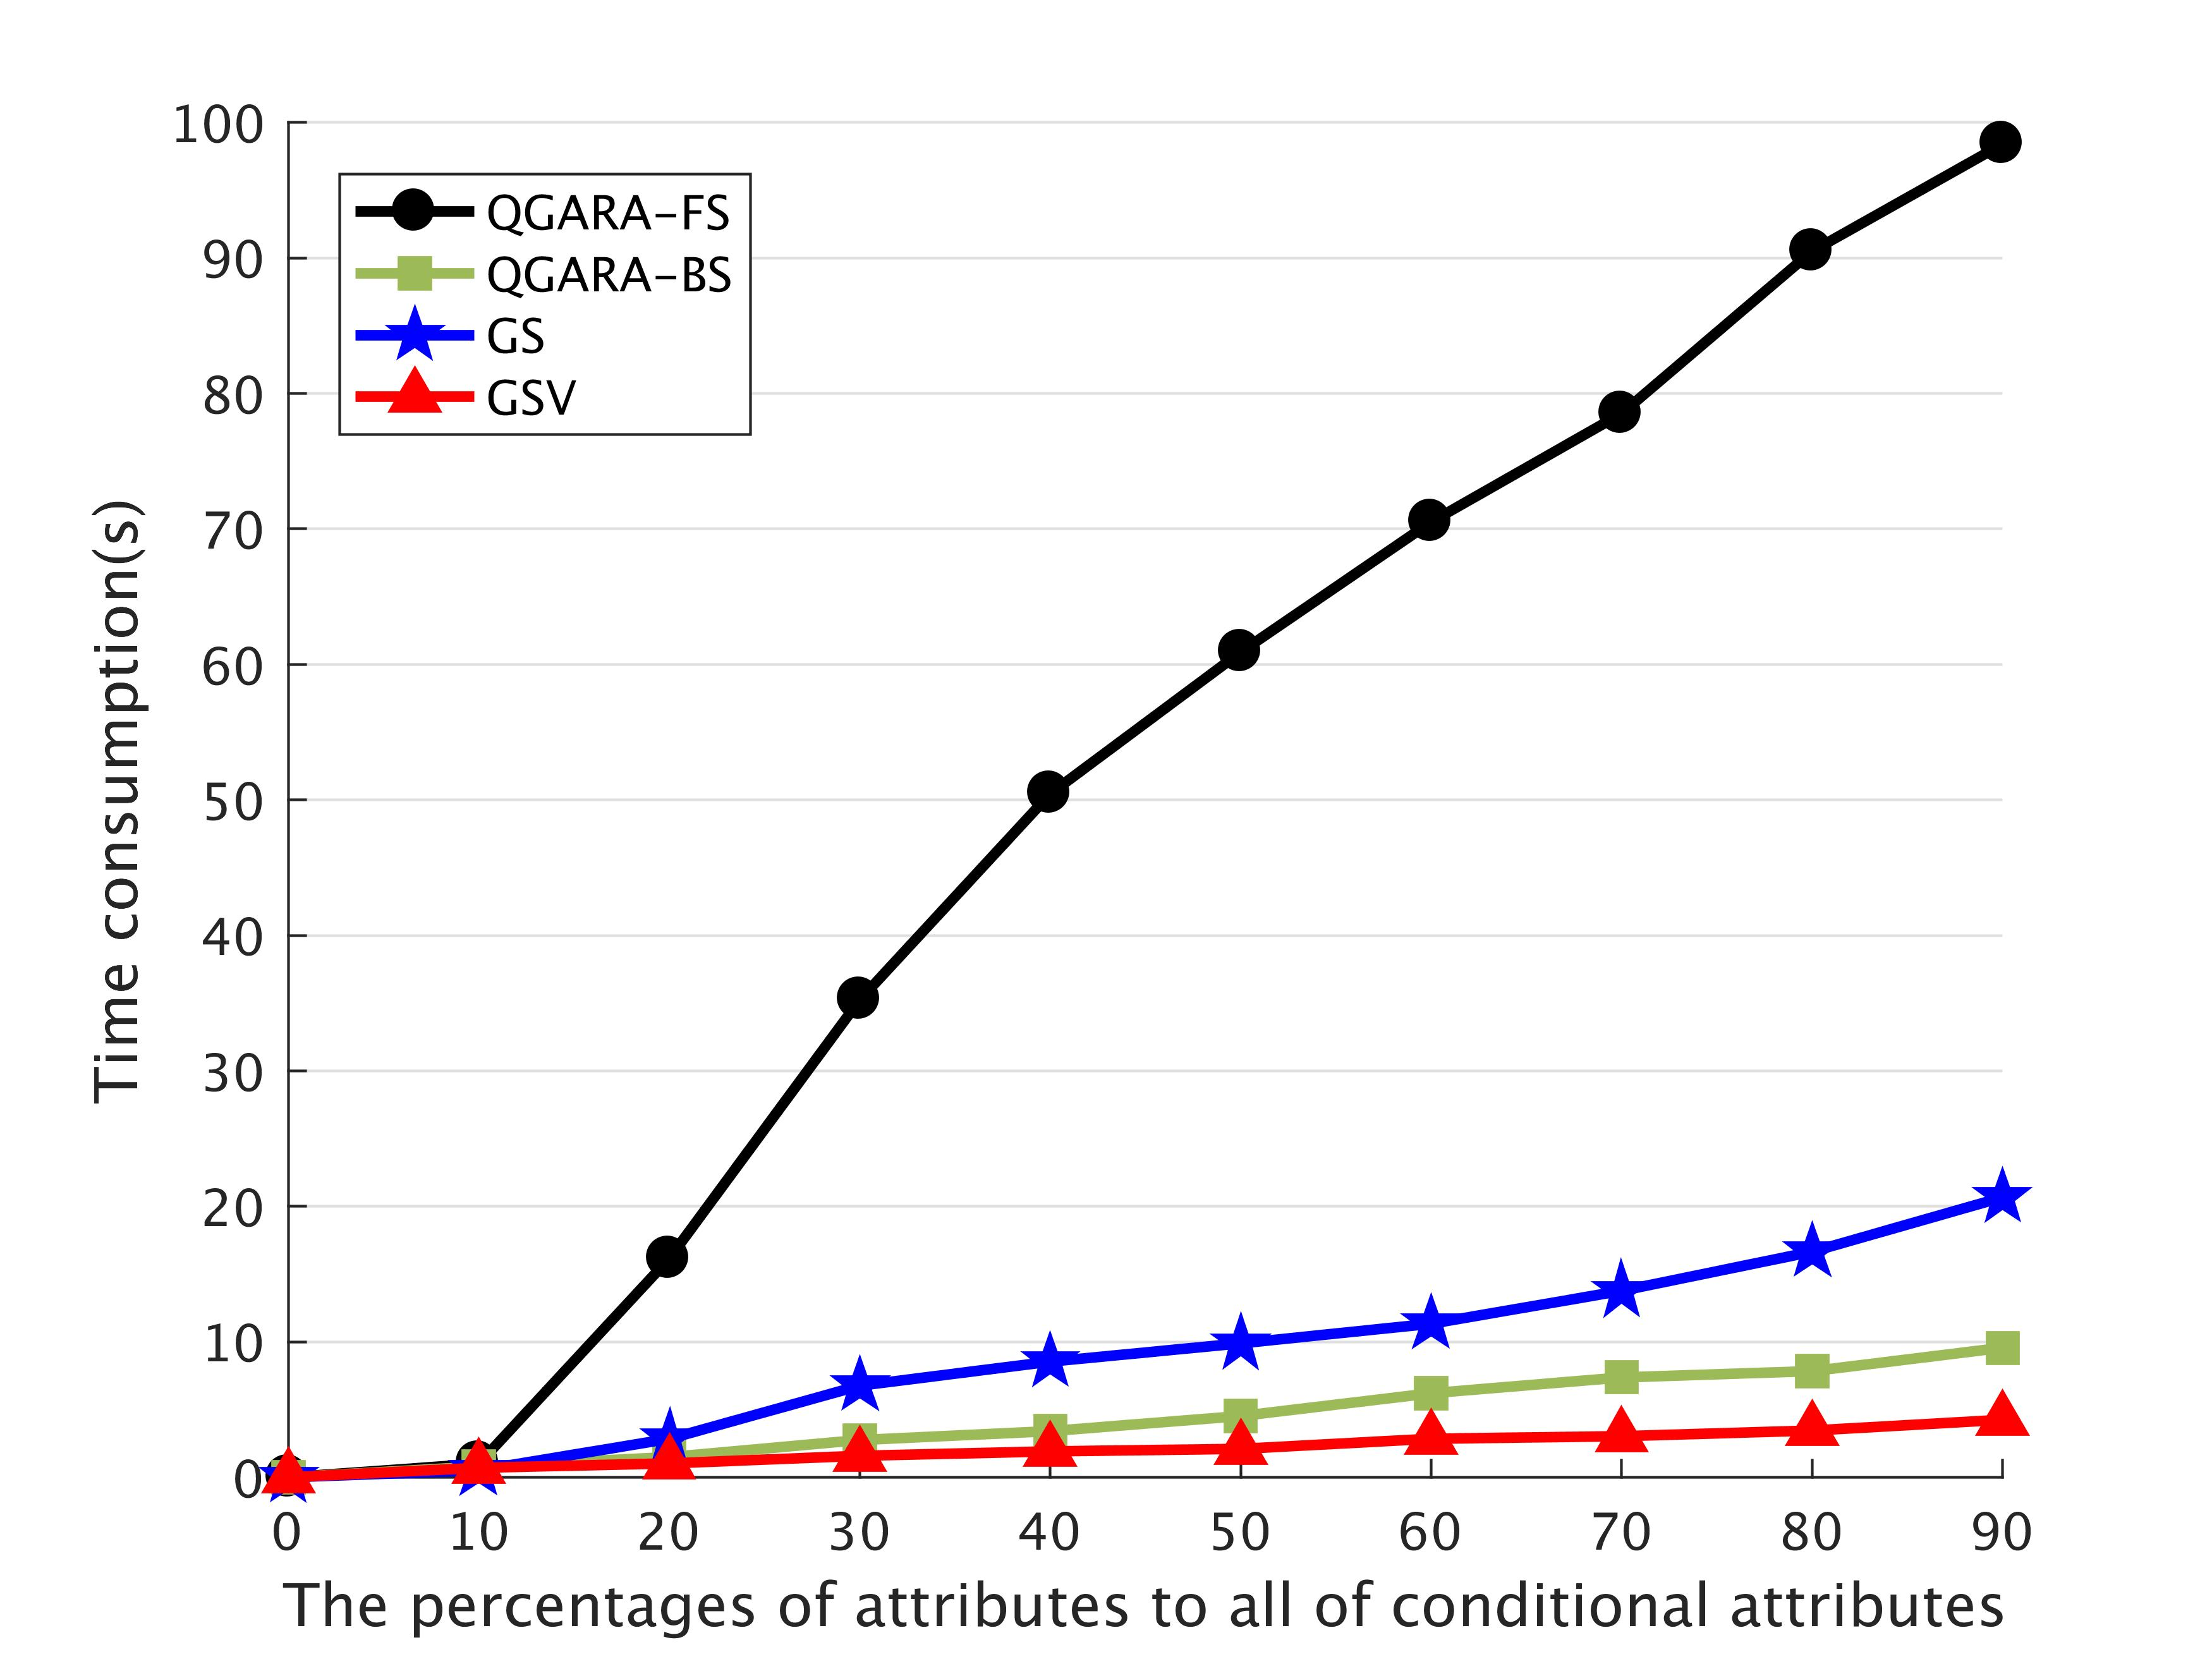
\includegraphics[width=5cm]{./Curve_attributes/9_dna_pos.jpg} 
			}
%			\subfigure[connect4]{
%				\label{Fig.sub2.12}
%				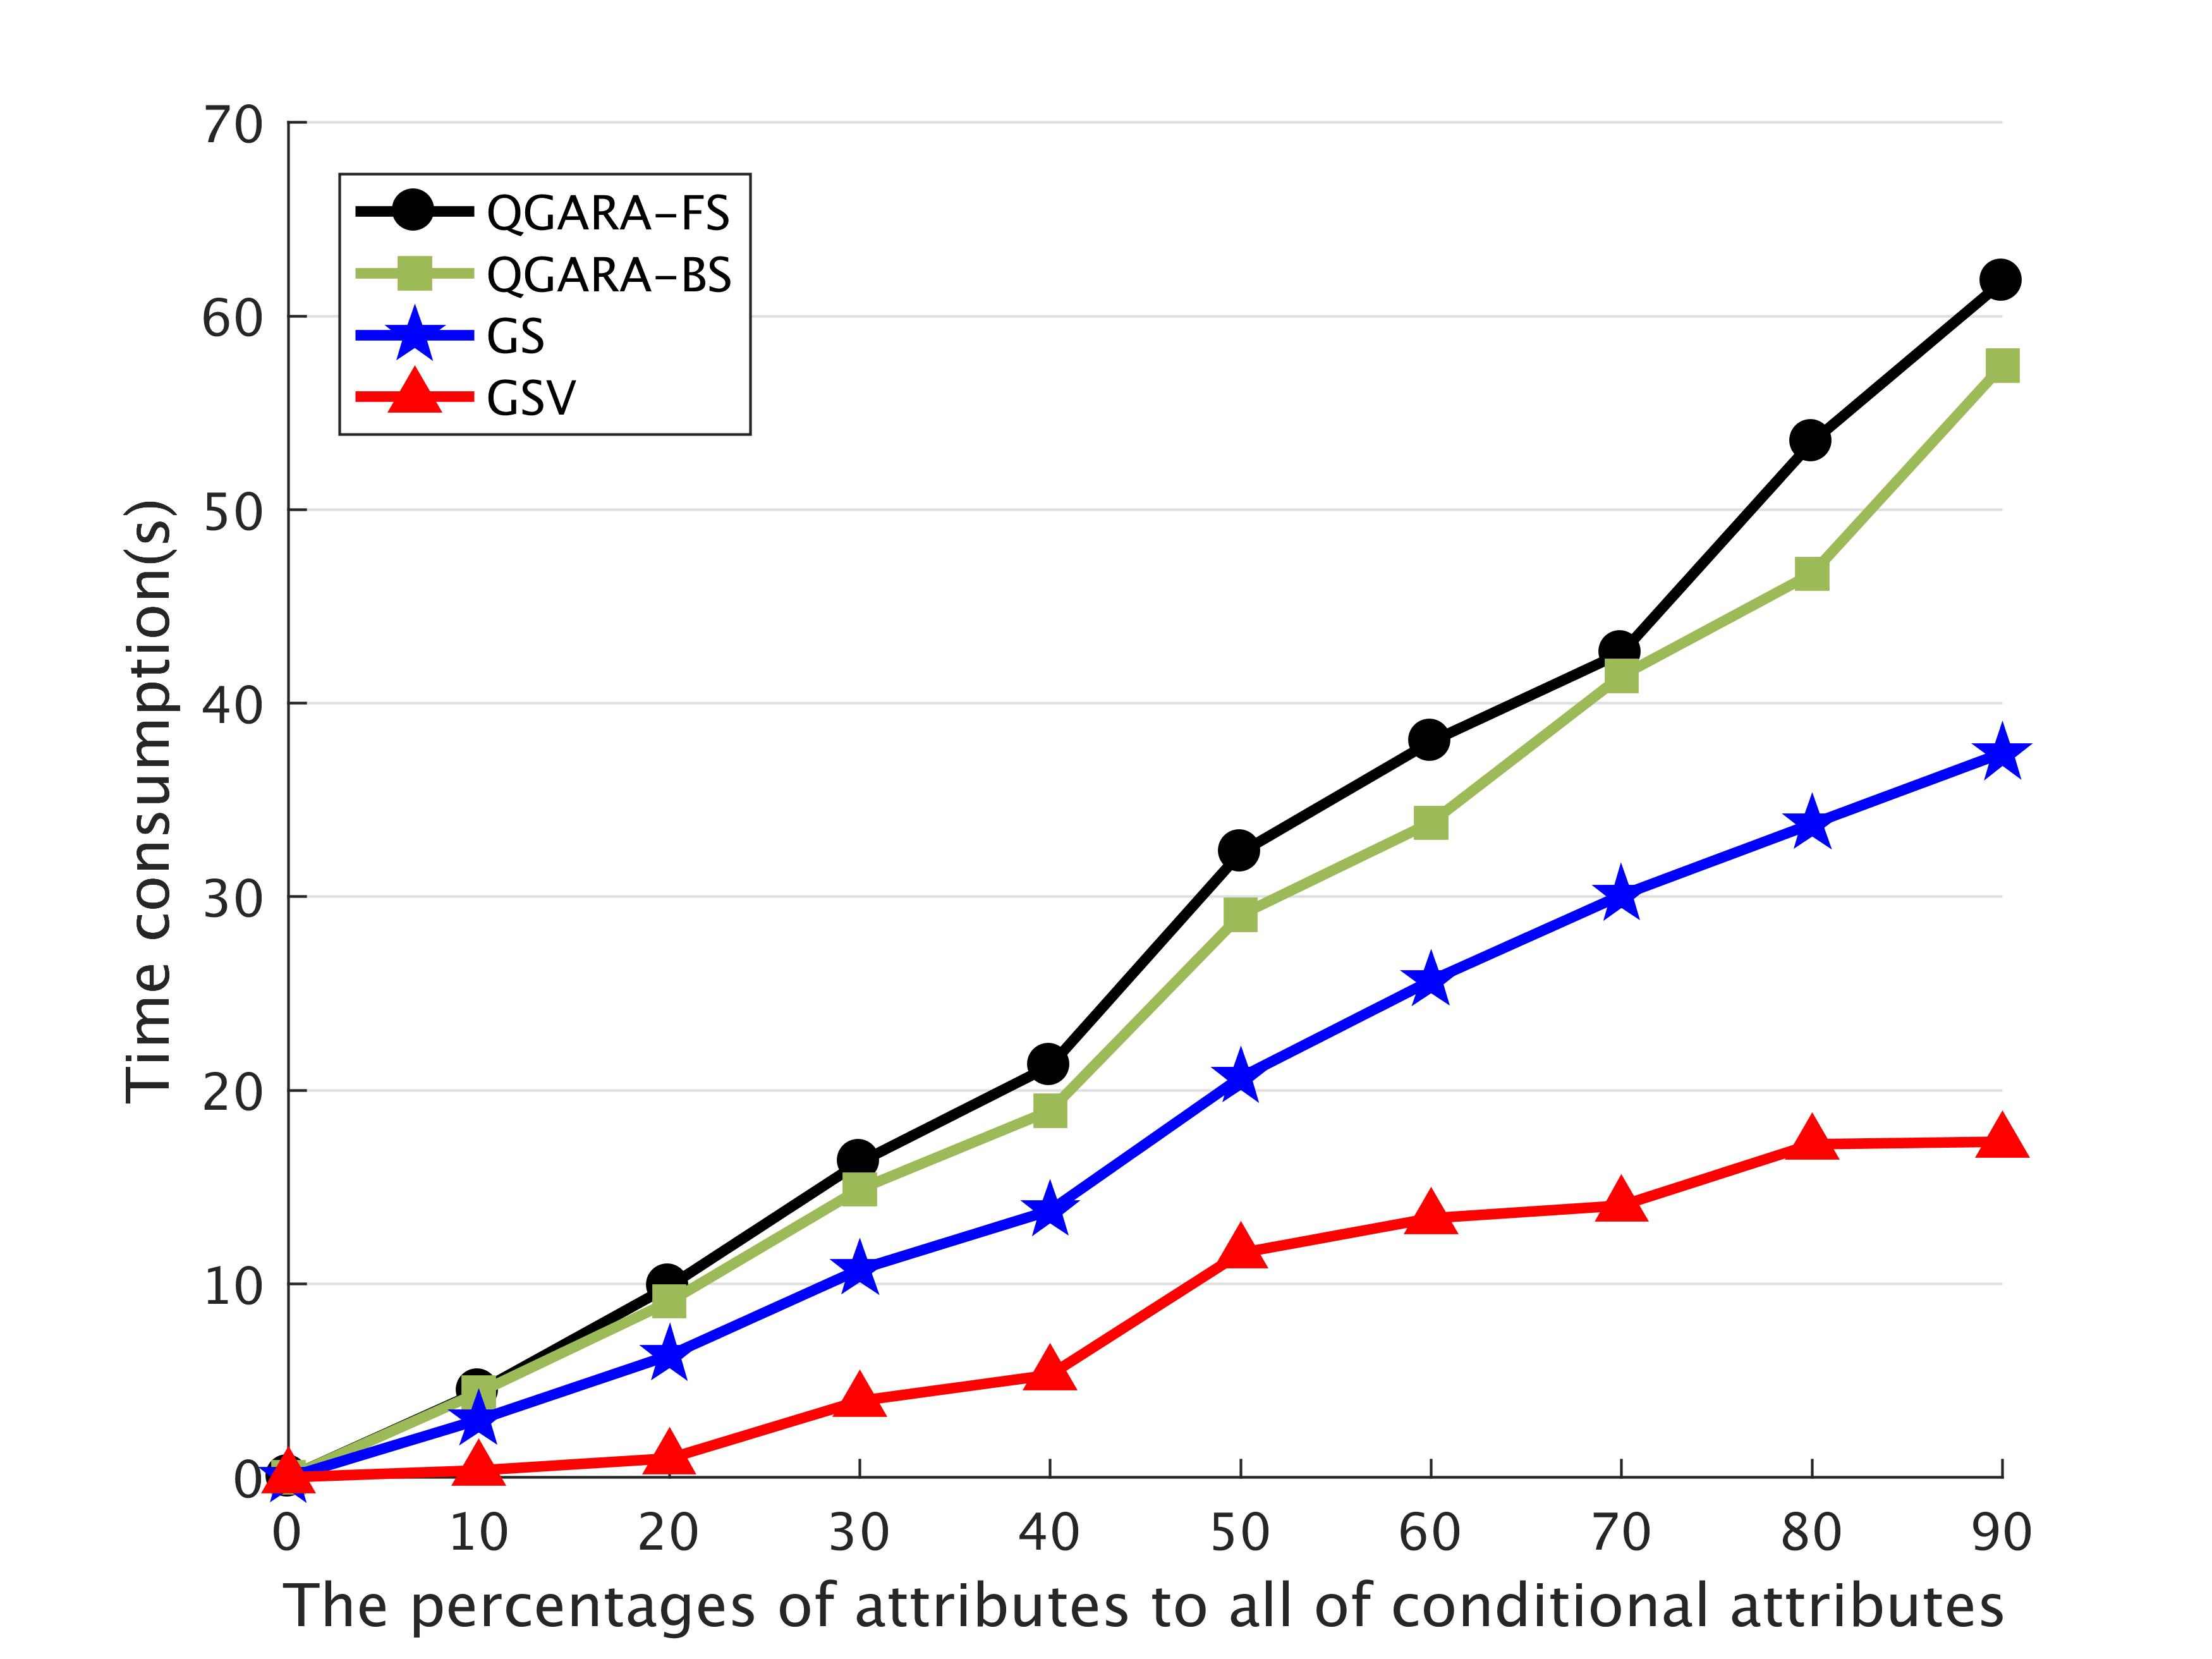
\includegraphics[width=5cm]{./Curve_attributes/10_connect4_pos.jpg} 
%			}
			\caption{Time of general reduction algorithms versus the size of attributes} 
			\label{TimeIncreaseAttributes}
		\end{figure}
		\par In Figure \ref{TimeIncreaseAttributes}, the x-coordinate pertains to the percentages of attributes to the conditional attributes of the data set, while the y-coordinate concerns the time consumption of algorithm. We token 8 data sets (Mushroom, Tic, Segmentation, Splice, Dermatology, Wdbc, CNAE9, and DNA) to verify the performance of the computational times of QGARA-FS, QGARA-BS, GS, and GSV. The result of QGARA-FS, QGARA-BS, GS, and GSV was similar to the result induced from Figure \ref{TimeIncreaseObjects}. The computational times of four algorithms increased with the increase of the number of attributes monotonously in most of the cases. When dealing with the same situation, the computational time of GSV was the minimum among the four algorithms.
%	\subsection{Comparison of reduction results for four general reduction algorithms}
%		\begin{table}[htbp]
%			\centering
%			\caption{Add caption}
%			\begin{tabular}{ccccc}
%				\hline
%				\multirow{2}[2]{*}{ID} & \multicolumn{4}{c}{The length of algorithm output} \\
%				& QGARA-FS & QGARA-BS & GS    & GSV \\
%				\hline
%				1     & \textbf{9} & \textbf{9} & \textbf{9} & \textbf{9} \\
%				2     & 7     & \textbf{5} & \textbf{5} & 10 \\
%				3     & \textbf{27} & 28    & \textbf{27} & 37 \\
%				4     & \textbf{8} & \textbf{8} & \textbf{8} & 17 \\
%				5     & \textbf{8} & \textbf{8} & \textbf{8} & \textbf{8} \\
%				6     & \textbf{10} & 11    & \textbf{10} & 14 \\
%				7     & \textbf{6} & 8     & 7     & 17 \\
%				8     & \textbf{6} & 8     & \textbf{6} & 9 \\
%				9     & \textbf{76} & 95    & 85    & 285 \\
%				10    & \textbf{25} & 48    & 32    & 81 \\
%				11    & \textbf{17} & 26    & 20    & 32 \\
%				12    & \textbf{34} & 41    & 35    & 41 \\
%				\hline
%			\end{tabular}%
%			\label{tab:addlabel}%
%		\end{table}%
%
%		\begin{table}[htbp]
%			\centering
%			\caption{Add caption}
%			\begin{tabular}{ccccc}
%				\hline
%				\multirow{2}[2]{*}{ID} & \multicolumn{4}{c}{The length of DRPR} \\
%				& QGARA-FS & QGARA-BS & GS    & GSV \\
%				\hline
%				1     & \textbf{9} & \textbf{9} & \textbf{9} & \textbf{9} \\
%				2     & \textbf{12} & \textbf{12} & \textbf{12} & 29 \\
%				3     & 28    & 28    & \textbf{27} & 37 \\
%				4     & \textbf{8} & \textbf{8} & \textbf{8} & 17 \\
%				5     & \textbf{8} & \textbf{8} & \textbf{8} & 8 \\
%				6     & \textbf{10} & 11    & \textbf{10} & 14 \\
%				7     & \textbf{6} & 8     & 7     & 17 \\
%				8     & \textbf{6} & 8     & \textbf{6} & 9 \\
%				9     & \textbf{76} & 95    & 85    & 285 \\
%				10    & \textbf{25} & 48    & 32    & 81 \\
%				11    & \textbf{17} & 26    & 20    & 32 \\
%				12    & \textbf{34} & 41    & 35    & 41 \\
%				\hline
%			\end{tabular}%
%			\label{tab:addlabel}%
%		\end{table}%
	\subsection{Comparison of classification accuracy for four general attribute reduction algorithms}
		\par To evaluate the effect of reduct obtained by different general reduction algorithms, we selected 10 data sets from Table \ref{uci} and utilized the original data and the corresponding reduced data that were generated by four algorithms (QGARA-FS, QGARA-BS, GS, and GSV) to train naive bayes and decision tree classifiers based on 10-fold cross-validation method. For naive bayes and decision tree classifier, we used its implementation in \cite{scikit-learn}. The classification accuracy to the raw data and reduced data generated by different algorithms were shown in Tables \ref{cadtd} to \ref{canbd}, where the column "Raw" denotes raw data, the boldface highlights the highest accuracy among different reduction algorithms, and the row "Average" represents average classification accuracy of reduction algorithm on 10 data sets.
		\begin{table}[htbp]
			\centering
			\caption{The classification accuracy of decision tree with PRPR found by four algorithms}
			\begin{tabular}{cccccc}
				\hline
				ID    & Raw   & QGARA-FS & QGARA-BS & GS    & GSV \\\hline
				2     & 0.551 & 0.603 & 0.608 & \textbf{0.614} & 0.574 \\
				3     & 0.896 & 0.894 & \textbf{0.898} & 0.897 & 0.896 \\
				4     & 0.942 & 0.937 & \textbf{0.94} & 0.935 & \textbf{0.94} \\
				5     & 0.69  & \textbf{0.687} & 0.686 & 0.682 & 0.68 \\
				6     & 0.896 & 0.648 & 0.453 & 0.762 & \textbf{0.801} \\
				7     & 0.942 & 0.598 & 0.735 & 0.803 & \textbf{0.87} \\
				8     & 0.93  & \textbf{0.937} & 0.905 & 0.907 & 0.926 \\
				9     & 0.864 & \textbf{0.874} & 0.856 & 0.87  & 0.872 \\
				11    & 0.903 & 0.858 & 0.492 & \textbf{0.874} & 0.576 \\
				12    & 0.475 & 0.474 & 0.465 & 0.477 & \textbf{0.478} \\\hline
				Average & 0.8089 & 0.751 & 0.7038 & \textbf{0.7821} & 0.7613 \\\hline
			\end{tabular}%
			\label{cadtp}%
		\end{table}%
		Obviously, for most of reduced data sets, reduced data can retain similar classification accuracy as the entire data set. 
		\begin{table}[htbp]
			\centering
			\caption{The classification accuracy of decision tree with DRPR found by four algorithms}
			\begin{tabular}{cccccc}
				\hline
				ID    & Raw   & QGARA-FS & QGARA-BS & GS    & GSV \\\hline
				2     & 0.551 & 0.555 & 0.551 & \textbf{0.558} & 0.551 \\
				3     & 0.896 & 0.896 & \textbf{0.898} & 0.896 & 0.896 \\
				4     & 0.942 & 0.937 & 0.938 & 0.936 & \textbf{0.939} \\
				5     & 0.69  & 0.68  & 0.681 & \textbf{0.684} & 0.672 \\
				6     & 0.896 & 0.645 & 0.453 & 0.756 & \textbf{0.806} \\
				7     & 0.942 & 0.604 & 0.743 & 0.798 & \textbf{0.867} \\
				8     & 0.93  & \textbf{0.937} & 0.91  & 0.914 & 0.931 \\
				9     & 0.864 & 0.872 & 0.86  & 0.87  & \textbf{0.874} \\
				11    & 0.903 & 0.859 & 0.496 & \textbf{0.869} & 0.589 \\
				12    & 0.475 & 0.478 & 0.465 & \textbf{0.479} & 0.477 \\\hline
				Average & 0.8089 & 0.7463 & 0.6995 & \textbf{0.776} & 0.7602 \\\hline
			\end{tabular}%
			\label{cadtd}%
		\end{table}%
		\par For Table \ref{cadtd}, the order of algorithms in the number of achieving the most classification accuracy is GSV(4) $>$ QGARA-FS(3) $>$ QGARA-BS(2) $>$ GS(2). However, GS achieves the best average classification accuracy on 10 data sets. That is to say, the steadiness of algorithms GSV, QGARA-FS, and GSV in classification accuracy is not good as GS. The order of algorithms in the average of classification accuracy on 10 data sets is GS(0.7821) $>$ GSV(0.7613) $>$ QGARA-FS(0.751) $>$ QGARA-BS(0.7038). GS and GSV perform better than QGARA-FS and QGARA-BS in the average classification accuracy. When comes to the reduced data generated by relative discernibility relation preservation reduct, GS performs the best in times of achieving the best classification. GS obtains the highest classification accuracy 6 times; GSV obtains the highest classification accuracy 5 times; QGARA-BS obtains the highest classification accuracy 2 times; QGARA-FS obtains the highest classification accuracy only 1 times; That is consistent with the order of the average classification accuracy on ten data sets, \emph{i.e.} GS(0.7367) $>$ GSV(0.7272) $>$ QGARA-BS(0.6986) $>$ QGARA-FS(0.6927). 
		\begin{table}[htbp]
			\centering
			\caption{The classification accuracy of naive bayes with PRPR found by four algorithms}
			\begin{tabular}{cccccc}
				\hline
				ID    & Raw   & QGARA-FS & QGARA-BS & GS    & GSV \\\hline
				2     & 0.649 & 0.557 & \textbf{0.65} & 0.565 & 0.582 \\
				3     & 0.777 & 0.885 & 0.895 & \textbf{0.896} & \textbf{0.896} \\
				4     & 0.603 & 0.575 & 0.57  & 0.575 & \textbf{0.605} \\
				5     & 0.682 & \textbf{0.682} & \textbf{0.682} & \textbf{0.682} & \textbf{0.682} \\
				6     & 0.792 & 0.545 & 0.519 & \textbf{0.657} & 0.576 \\
				7     & 0.977 & 0.602 & 0.769 & 0.763 & \textbf{0.933} \\
				8     & 0.902 & 0.804 & 0.865 & \textbf{0.889} & 0.874 \\
				9     & 0.949 & 0.909 & 0.901 & 0.907 & \textbf{0.933} \\
				11    & 0.924 & 0.767 & 0.535 & \textbf{0.827} & 0.594 \\
				12    & 0.597 & 0.601 & 0.599 & \textbf{0.606} & 0.597 \\\hline
				Average & 0.7852 & 0.6927 & 0.6985 & \textbf{0.7367} & 0.7272 \\\hline
			\end{tabular}%
			\label{canbp}%
		\end{table}%
		\par In the classification accuracy results of Naive Bayes on reduced data generated by positive region preservation reduct and relative discernibility relation preservation reduct, GS is still the best one in the classification accuracy on 10 data sets, and GSV is the next one. That is to say, the general attribute reduction algorithms proposed in this study, \emph{i.e.} GS and GSV, are better and more steady than the existing general attribute reduction algorithms. 
		% Table generated by Excel2LaTeX from sheet 'naiveBayes_pos'
		
		
		% Table generated by Excel2LaTeX from sheet 'naiveBayes_ind'
		\begin{table}[htbp]
			\centering
			\caption{The classification accuracy of naive bayes with DRPR found by four algorithms}
			\begin{tabular}{cccccc}
				\hline
				ID    & Raw   & QGARA-FS & QGARA-BS & GS    & GSV \\\hline
				2     & 0.649 & 0.595 & \textbf{0.642} & 0.595 & 0.636 \\
				3     & 0.777 & 0.891 & 0.895 & \textbf{0.896} & \textbf{0.896} \\
				4     & 0.603 & 0.575 & 0.57  & 0.575 & \textbf{0.605} \\
				5     & 0.682 & \textbf{0.682} & \textbf{0.682} & \textbf{0.682} & \textbf{0.682} \\
				6     & 0.792 & 0.545 & 0.519 & \textbf{0.657} & 0.576 \\
				7     & 0.977 & 0.602 & 0.769 & 0.763 & \textbf{0.933} \\
				8     & 0.902 & 0.804 & 0.865 & \textbf{0.889} & 0.874 \\
				9     & 0.949 & 0.909 & 0.901 & 0.907 & \textbf{0.933} \\
				11    & 0.924 & 0.767 & 0.535 & \textbf{0.827} & 0.594 \\
				12    & 0.597 & 0.601 & 0.599 & \textbf{0.606} & 0.597 \\\hline
				Average & 0.7852 & 0.6971 & 0.6977 & \textbf{0.7397} & 0.7326 \\\hline
			\end{tabular}%
			\label{canbd}%
		\end{table}%

	\par In the experimental part, we made a series of comparisons between the general attribute reduction algorithms proposed in this study and the existing general attribute reduction algorithms, and we had got conclusion listed as follows:
	\\\indent\rm{(1)} In time consumption of the algorithm to obtain reducts, GS performed well in dealing with small-scale data. When processing large-scale data sets, GSV and QGARA-BS were good choices for attribute reduction.
	\\\indent\rm{(2)} To get the classification accuracy closed to that of the original data set, taking GS or GSV as the attribute reduction method was a reasonable decision.
		
\section{Conclusion}
	\par In this study, we focus on the efficient general reduction approach to obtain five types of reducts on the complete inconsistent decision table. We introduce a concept termed granularity space and represent five types of reducts in granularity space. Based on the unified representation, we develop two quick general reduction algorithms. In comparison with the existing general reduction algorithms, the proposed algorithms have two advantages as follows.
	\\\indent(1) The proposed algorithms are more efficient. In the process of attribute reduction, GS can reduce one half of the computation time of QGARA-FS and GSV can reduce over one half of the computation time of QGARA-BS.
	\\\indent(2) The proposed algorithms perform steadier in the classification accuracy. The average classification accuracy of decision tree classifier and naive bayes classifier trained on reduced data generated by GS and GSV is 3 percent higher than that trained on reduced data generated by QGARA-FS or QGARA-BS.
	\\\indent However, it is notable that the general reduction definitions and algorithms proposed in this paper are only suitable for the complete decision table. There exists many generalized decision tables, such as incomplete decision tables, interval-valued decision tables. Research on the extension of granularity space for the generalized decision table will be investigated in future work.  
\section*{Acknowledgement}
	The work is partially supported by the National Key Research and Development Project (No. 213), the National Nature Science Foundation of China (No.  61976160, No. 61976160, No. 61673301) and Key Lab of Information Network Security, Ministry of Public Security (No. C18608).
\section*{References}
\bibliographystyle{plain}
\bibliography{mybib}

%\begin{appendices}
%	some of content here.
%\end{appendices}
\end{document}